\documentclass{book}
\usepackage[a4paper,top=2.5cm,bottom=2.5cm,left=2.5cm,right=2.5cm]{geometry}
\usepackage{makeidx}
\usepackage{natbib}
\usepackage{graphicx}
\usepackage{multicol}
\usepackage{float}
\usepackage{listings}
\usepackage{color}
\usepackage{ifthen}
\usepackage[table]{xcolor}
\usepackage{textcomp}
\usepackage{alltt}
\usepackage{ifpdf}
\ifpdf
\usepackage[pdftex,
            pagebackref=true,
            colorlinks=true,
            linkcolor=blue,
            unicode
           ]{hyperref}
\else
\usepackage[ps2pdf,
            pagebackref=true,
            colorlinks=true,
            linkcolor=blue,
            unicode
           ]{hyperref}
\usepackage{pspicture}
\fi
\usepackage[utf8]{inputenc}
\usepackage{mathptmx}
\usepackage[scaled=.90]{helvet}
\usepackage{courier}
\usepackage{sectsty}
\usepackage{amssymb}
\usepackage[titles]{tocloft}
\usepackage{doxygen}
\lstset{language=C++,inputencoding=utf8,basicstyle=\footnotesize,breaklines=true,breakatwhitespace=true,tabsize=4,numbers=left }
\makeindex
\setcounter{tocdepth}{3}
\renewcommand{\footrulewidth}{0.4pt}
\renewcommand{\familydefault}{\sfdefault}
\hfuzz=15pt
\setlength{\emergencystretch}{15pt}
\hbadness=750
\tolerance=750
\begin{document}
\hypersetup{pageanchor=false,citecolor=blue}
\begin{titlepage}
\vspace*{7cm}
\begin{center}
{\Large Tri\-Engine2\-D \\[1ex]\large v0.\-0.\-7 }\\
\vspace*{1cm}
{\large Generated by Doxygen 1.8.3.1}\\
\vspace*{0.5cm}
{\small Mon Feb 11 2013 02:06:50}\\
\end{center}
\end{titlepage}
\clearemptydoublepage
\pagenumbering{roman}
\tableofcontents
\clearemptydoublepage
\pagenumbering{arabic}
\hypersetup{pageanchor=true,citecolor=blue}
\chapter{Main Page}
\label{index}\hypertarget{index}{}2\-D general-\/purpose engine in C\#/\-Open\-G\-L

\subsection*{I\-R\-C}

\hyperlink{namespace_tri_devs}{Tri\-Devs} has an I\-R\-C channel, feel free to hop in if you have a question about anything\-: {\bfseries Server\-:} irc.\-kottnet.\-net {\bfseries Port\-:} 6667, 6697 (S\-S\-L) {\bfseries Channel\-:} \hyperlink{namespace_tri_devs}{Tri\-Devs}

The channel topic contains further info.

\subsection*{License}

Copyright © 2013 by \href{https://github.com/Sharparam}{\tt Adam Hellberg}, \href{https://github.com/Vijfhoek}{\tt Sijmen Schoon} and \href{https://github.com/anidude}{\tt Preston Shumway}.

Tri\-Engine2\-D is licensed under the \href{http://opensource.org/licenses/MIT}{\tt M\-I\-T License}, more info can be found in the {\bfseries L\-I\-C\-E\-N\-S\-E} file.

\subsection*{Contributing}

You are free to fork this project and make your own changes, as long as you follow the M\-I\-T License.

If you want to make a pull request, please do so to the \href{https://github.com/TriDevs/TriEngine2D}{\tt main project} and not any of the \char`\"{}official\char`\"{} forks.

For your pull request to be accepted, please follow our coding style\-:
\begin{DoxyItemize}
\item Indent with 4 spaces, not tabs.
\item Curly braces placed on next line.
\item All {\bfseries public} methods, accessors and members must be properly documented.
\item Use sensible variable names that describe what they are for.
\item Method declarations written as\-:
\end{DoxyItemize}

```c\# public void Hello(string world) ```


\begin{DoxyItemize}
\item If your method accepts many parameters, it can be useful to put parameters on separate lines, as per this style\-:
\end{DoxyItemize}

```c\# public void Hello(string world, bool print) ```


\begin{DoxyItemize}
\item Please write tests for your code (not strictly required, but it's a plus)
\end{DoxyItemize}

By looking through the current source code, you should be able to get a good understanding of the formatting we use.

If you're using Visual Studio, you can change the indent behaviour by going to\-: {\bfseries Tools} -\/$>$ {\bfseries Options} -\/$>$ {\bfseries Text Editor} -\/$>$ {\bfseries C\#} -\/$>$ {\bfseries Tabs} and make sure \char`\"{}\-Insert spaces\char`\"{} is checked.

If you write tests for your code, please place these tests in their own project\-: \char`\"{}\&lt; $<$strong$>$\-Namespace$<$/strong$>$ \&gt;.\-Tests\char`\"{}, create said project if it does not exist (of type Class Library).

We use N\-Unit as test framework, feel free to use something else if you want to, but make sure you document what framework you are using and that it is freely available for anyone to obtain.

\subsection*{Dependencies}

Tri\-Engine2\-D depends on \href{http://logging.apache.org/log4net/}{\tt log4net}, which is included in the {\bfseries libs/log4net} folder.

Tri\-Engine2\-D depends on \href{http://www.opentk.com/}{\tt Open\-T\-K}, this is not included and you will have to build/install it yourself. Open\-T\-K depends on Open\-G\-L drivers being installed, they are usually in your normal video card drivers.

Tri\-Engine2\-D depends on \href{http://json.codeplex.com/}{\tt Json.\-N\-E\-T}, this is not included, but is specified in the Nu\-Get package config. If you \href{http://docs.nuget.org/docs/workflows/using-nuget-without-committing-packages#Using_NuGet_without_committing_packages_to_source_control}{\tt properly configure your Nu\-Get settings}, Nu\-Get will automatically download Json.\-N\-E\-T when building any projects that depend on it.

If you want to run the tests you will need to have \href{http://www.nunit.org/}{\tt N\-Unit} installed. 
\chapter{Namespace Index}
\section{Namespace List}
Here is a list of all namespaces with brief descriptions\-:\begin{DoxyCompactList}
\item\contentsline{section}{\hyperlink{namespace_tri_devs}{Tri\-Devs} }{\pageref{namespace_tri_devs}}{}
\item\contentsline{section}{\hyperlink{namespace_tri_devs_1_1_tri_engine2_d}{Tri\-Devs.\-Tri\-Engine2\-D} }{\pageref{namespace_tri_devs_1_1_tri_engine2_d}}{}
\item\contentsline{section}{\hyperlink{namespace_tri_devs_1_1_tri_engine2_d_1_1_audio}{Tri\-Devs.\-Tri\-Engine2\-D.\-Audio} }{\pageref{namespace_tri_devs_1_1_tri_engine2_d_1_1_audio}}{}
\item\contentsline{section}{\hyperlink{namespace_tri_devs_1_1_tri_engine2_d_1_1_extensions}{Tri\-Devs.\-Tri\-Engine2\-D.\-Extensions} }{\pageref{namespace_tri_devs_1_1_tri_engine2_d_1_1_extensions}}{}
\item\contentsline{section}{\hyperlink{namespace_tri_devs_1_1_tri_engine2_d_1_1_graphics}{Tri\-Devs.\-Tri\-Engine2\-D.\-Graphics} }{\pageref{namespace_tri_devs_1_1_tri_engine2_d_1_1_graphics}}{}
\item\contentsline{section}{\hyperlink{namespace_tri_devs_1_1_tri_engine2_d_1_1_helpers}{Tri\-Devs.\-Tri\-Engine2\-D.\-Helpers} }{\pageref{namespace_tri_devs_1_1_tri_engine2_d_1_1_helpers}}{}
\item\contentsline{section}{\hyperlink{namespace_tri_devs_1_1_tri_engine2_d_1_1_input}{Tri\-Devs.\-Tri\-Engine2\-D.\-Input} }{\pageref{namespace_tri_devs_1_1_tri_engine2_d_1_1_input}}{}
\item\contentsline{section}{\hyperlink{namespace_tri_devs_1_1_tri_engine2_d_1_1_input_1_1_events}{Tri\-Devs.\-Tri\-Engine2\-D.\-Input.\-Events} }{\pageref{namespace_tri_devs_1_1_tri_engine2_d_1_1_input_1_1_events}}{}
\item\contentsline{section}{\hyperlink{namespace_tri_devs_1_1_tri_engine2_d_1_1_interfaces}{Tri\-Devs.\-Tri\-Engine2\-D.\-Interfaces} }{\pageref{namespace_tri_devs_1_1_tri_engine2_d_1_1_interfaces}}{}
\item\contentsline{section}{\hyperlink{namespace_tri_devs_1_1_tri_engine2_d_1_1_logging}{Tri\-Devs.\-Tri\-Engine2\-D.\-Logging} }{\pageref{namespace_tri_devs_1_1_tri_engine2_d_1_1_logging}}{}
\item\contentsline{section}{\hyperlink{namespace_tri_devs_1_1_tri_engine2_d_1_1_native}{Tri\-Devs.\-Tri\-Engine2\-D.\-Native} }{\pageref{namespace_tri_devs_1_1_tri_engine2_d_1_1_native}}{}
\item\contentsline{section}{\hyperlink{namespace_tri_devs_1_1_tri_engine2_d_1_1_serializing}{Tri\-Devs.\-Tri\-Engine2\-D.\-Serializing} }{\pageref{namespace_tri_devs_1_1_tri_engine2_d_1_1_serializing}}{}
\item\contentsline{section}{\hyperlink{namespace_tri_devs_1_1_tri_engine2_d_1_1_shaders}{Tri\-Devs.\-Tri\-Engine2\-D.\-Shaders} }{\pageref{namespace_tri_devs_1_1_tri_engine2_d_1_1_shaders}}{}
\item\contentsline{section}{\hyperlink{namespace_tri_devs_1_1_tri_engine2_d_1_1_state_management}{Tri\-Devs.\-Tri\-Engine2\-D.\-State\-Management} }{\pageref{namespace_tri_devs_1_1_tri_engine2_d_1_1_state_management}}{}
\item\contentsline{section}{\hyperlink{namespace_tri_devs_1_1_tri_engine2_d_1_1_text}{Tri\-Devs.\-Tri\-Engine2\-D.\-Text} }{\pageref{namespace_tri_devs_1_1_tri_engine2_d_1_1_text}}{}
\item\contentsline{section}{\hyperlink{namespace_tri_devs_1_1_tri_engine2_d_1_1_u_i}{Tri\-Devs.\-Tri\-Engine2\-D.\-U\-I} }{\pageref{namespace_tri_devs_1_1_tri_engine2_d_1_1_u_i}}{}
\item\contentsline{section}{\hyperlink{namespace_tri_devs_1_1_tri_engine2_d_1_1_u_i_1_1_events}{Tri\-Devs.\-Tri\-Engine2\-D.\-U\-I.\-Events} }{\pageref{namespace_tri_devs_1_1_tri_engine2_d_1_1_u_i_1_1_events}}{}
\end{DoxyCompactList}

\chapter{Hierarchical Index}
\section{Class Hierarchy}
This inheritance list is sorted roughly, but not completely, alphabetically\-:\begin{DoxyCompactList}
\item \contentsline{section}{Tri\-Devs.\-Tri\-Engine2\-D.\-U\-I.\-Color}{\pageref{struct_tri_devs_1_1_tri_engine2_d_1_1_u_i_1_1_color}}{}
\item \contentsline{section}{Tri\-Devs.\-Tri\-Engine2\-D.\-Extensions.\-Enumeration\-Extensions}{\pageref{class_tri_devs_1_1_tri_engine2_d_1_1_extensions_1_1_enumeration_extensions}}{}
\item Event\-Args\begin{DoxyCompactList}
\item \contentsline{section}{Tri\-Devs.\-Tri\-Engine2\-D.\-Input.\-Events.\-Key\-Char\-Event\-Args}{\pageref{class_tri_devs_1_1_tri_engine2_d_1_1_input_1_1_events_1_1_key_char_event_args}}{}
\item \contentsline{section}{Tri\-Devs.\-Tri\-Engine2\-D.\-Input.\-Events.\-Key\-Event\-Args}{\pageref{class_tri_devs_1_1_tri_engine2_d_1_1_input_1_1_events_1_1_key_event_args}}{}
\end{DoxyCompactList}
\item \contentsline{section}{Tri\-Devs.\-Tri\-Engine2\-D.\-Native.\-Helpers}{\pageref{class_tri_devs_1_1_tri_engine2_d_1_1_native_1_1_helpers}}{}
\item \contentsline{section}{Tri\-Devs.\-Tri\-Engine2\-D.\-U\-I.\-I\-Control}{\pageref{interface_tri_devs_1_1_tri_engine2_d_1_1_u_i_1_1_i_control}}{}
\begin{DoxyCompactList}
\item \contentsline{section}{Tri\-Devs.\-Tri\-Engine2\-D.\-U\-I.\-Control}{\pageref{class_tri_devs_1_1_tri_engine2_d_1_1_u_i_1_1_control}}{}
\begin{DoxyCompactList}
\item \contentsline{section}{Tri\-Devs.\-Tri\-Engine2\-D.\-U\-I.\-Label}{\pageref{class_tri_devs_1_1_tri_engine2_d_1_1_u_i_1_1_label}}{}
\begin{DoxyCompactList}
\item \contentsline{section}{Tri\-Devs.\-Tri\-Engine2\-D.\-U\-I.\-Link\-Label}{\pageref{class_tri_devs_1_1_tri_engine2_d_1_1_u_i_1_1_link_label}}{}
\end{DoxyCompactList}
\end{DoxyCompactList}
\end{DoxyCompactList}
\item I\-Disposable\begin{DoxyCompactList}
\item \contentsline{section}{Tri\-Devs.\-Tri\-Engine2\-D.\-Audio.\-I\-Audio\-Manager}{\pageref{interface_tri_devs_1_1_tri_engine2_d_1_1_audio_1_1_i_audio_manager}}{}
\begin{DoxyCompactList}
\item \contentsline{section}{Tri\-Devs.\-Tri\-Engine2\-D.\-Audio.\-Audio\-Manager}{\pageref{class_tri_devs_1_1_tri_engine2_d_1_1_audio_1_1_audio_manager}}{}
\item \contentsline{section}{Tri\-Devs.\-Tri\-Engine2\-D.\-Audio.\-Null\-Audio\-Manager}{\pageref{class_tri_devs_1_1_tri_engine2_d_1_1_audio_1_1_null_audio_manager}}{}
\end{DoxyCompactList}
\item \contentsline{section}{Tri\-Devs.\-Tri\-Engine2\-D.\-Audio.\-I\-Song}{\pageref{interface_tri_devs_1_1_tri_engine2_d_1_1_audio_1_1_i_song}}{}
\begin{DoxyCompactList}
\item \contentsline{section}{Tri\-Devs.\-Tri\-Engine2\-D.\-Audio.\-Null\-Song}{\pageref{class_tri_devs_1_1_tri_engine2_d_1_1_audio_1_1_null_song}}{}
\item \contentsline{section}{Tri\-Devs.\-Tri\-Engine2\-D.\-Audio.\-Song}{\pageref{class_tri_devs_1_1_tri_engine2_d_1_1_audio_1_1_song}}{}
\end{DoxyCompactList}
\item \contentsline{section}{Tri\-Devs.\-Tri\-Engine2\-D.\-Audio.\-I\-Sound}{\pageref{interface_tri_devs_1_1_tri_engine2_d_1_1_audio_1_1_i_sound}}{}
\begin{DoxyCompactList}
\item \contentsline{section}{Tri\-Devs.\-Tri\-Engine2\-D.\-Audio.\-Null\-Sound}{\pageref{class_tri_devs_1_1_tri_engine2_d_1_1_audio_1_1_null_sound}}{}
\item \contentsline{section}{Tri\-Devs.\-Tri\-Engine2\-D.\-Audio.\-Sound}{\pageref{class_tri_devs_1_1_tri_engine2_d_1_1_audio_1_1_sound}}{}
\end{DoxyCompactList}
\end{DoxyCompactList}
\item \contentsline{section}{Tri\-Devs.\-Tri\-Engine2\-D.\-Interfaces.\-I\-Drawable}{\pageref{interface_tri_devs_1_1_tri_engine2_d_1_1_interfaces_1_1_i_drawable}}{}
\item \contentsline{section}{Tri\-Devs.\-Tri\-Engine2\-D.\-Input.\-I\-Input\-Manager}{\pageref{interface_tri_devs_1_1_tri_engine2_d_1_1_input_1_1_i_input_manager}}{}
\begin{DoxyCompactList}
\item \contentsline{section}{Tri\-Devs.\-Tri\-Engine2\-D.\-Input.\-Input\-Manager}{\pageref{class_tri_devs_1_1_tri_engine2_d_1_1_input_1_1_input_manager}}{}
\item \contentsline{section}{Tri\-Devs.\-Tri\-Engine2\-D.\-Input.\-Null\-Input\-Manager}{\pageref{class_tri_devs_1_1_tri_engine2_d_1_1_input_1_1_null_input_manager}}{}
\end{DoxyCompactList}
\item \contentsline{section}{Tri\-Devs.\-Tri\-Engine2\-D.\-Helpers.\-I\-O}{\pageref{class_tri_devs_1_1_tri_engine2_d_1_1_helpers_1_1_i_o}}{}
\item \contentsline{section}{Tri\-Devs.\-Tri\-Engine2\-D.\-Logging.\-Log\-Manager}{\pageref{class_tri_devs_1_1_tri_engine2_d_1_1_logging_1_1_log_manager}}{}
\item \contentsline{section}{Tri\-Devs.\-Tri\-Engine2\-D.\-Helpers.\-Math}{\pageref{class_tri_devs_1_1_tri_engine2_d_1_1_helpers_1_1_math}}{}
\item \contentsline{section}{Tri\-Devs.\-Tri\-Engine2\-D.\-Point$<$ T $>$}{\pageref{struct_tri_devs_1_1_tri_engine2_d_1_1_point_3_01_t_01_4}}{}
\item \contentsline{section}{Tri\-Devs.\-Tri\-Engine2\-D.\-Serializing.\-Serializer}{\pageref{class_tri_devs_1_1_tri_engine2_d_1_1_serializing_1_1_serializer}}{}
\item \contentsline{section}{Tri\-Devs.\-Tri\-Engine2\-D.\-Services}{\pageref{class_tri_devs_1_1_tri_engine2_d_1_1_services}}{}
\item \contentsline{section}{Tri\-Devs.\-Tri\-Engine2\-D.\-Extensions.\-String\-Extensions}{\pageref{class_tri_devs_1_1_tri_engine2_d_1_1_extensions_1_1_string_extensions}}{}
\item \contentsline{section}{Tri\-Devs.\-Tri\-Engine2\-D.\-Helpers.\-Threading}{\pageref{class_tri_devs_1_1_tri_engine2_d_1_1_helpers_1_1_threading}}{}
\item \contentsline{section}{Tri\-Devs.\-Tri\-Engine2\-D.\-Version}{\pageref{class_tri_devs_1_1_tri_engine2_d_1_1_version}}{}
\item \contentsline{section}{Tri\-Devs.\-Tri\-Engine2\-D.\-Native.\-Win\-A\-P\-I}{\pageref{class_tri_devs_1_1_tri_engine2_d_1_1_native_1_1_win_a_p_i}}{}
\end{DoxyCompactList}

\chapter{Class Index}
\section{Class List}
Here are the classes, structs, unions and interfaces with brief descriptions\-:\begin{DoxyCompactList}
\item\contentsline{section}{\hyperlink{class_tri_devs_1_1_tri_engine2_d_1_1_audio_1_1_audio_manager}{Tri\-Devs.\-Tri\-Engine2\-D.\-Audio.\-Audio\-Manager} \\*Class to manage engine audio. }{\pageref{class_tri_devs_1_1_tri_engine2_d_1_1_audio_1_1_audio_manager}}{}
\item\contentsline{section}{\hyperlink{struct_tri_devs_1_1_tri_engine2_d_1_1_color}{Tri\-Devs.\-Tri\-Engine2\-D.\-Color} \\*Represents an R\-G\-B\-A color that can be used with \hyperlink{namespace_tri_devs_1_1_tri_engine2_d}{Tri\-Engine2\-D}. }{\pageref{struct_tri_devs_1_1_tri_engine2_d_1_1_color}}{}
\item\contentsline{section}{\hyperlink{class_tri_devs_1_1_tri_engine2_d_1_1_u_i_1_1_control}{Tri\-Devs.\-Tri\-Engine2\-D.\-U\-I.\-Control} \\*Base control class that all other controls inherits from. Defines basic \hyperlink{namespace_tri_devs_1_1_tri_engine2_d_1_1_u_i}{U\-I} control behaviour. }{\pageref{class_tri_devs_1_1_tri_engine2_d_1_1_u_i_1_1_control}}{}
\item\contentsline{section}{\hyperlink{class_tri_devs_1_1_tri_engine2_d_1_1_u_i_1_1_control_manager}{Tri\-Devs.\-Tri\-Engine2\-D.\-U\-I.\-Control\-Manager} \\*\hyperlink{class_tri_devs_1_1_tri_engine2_d_1_1_u_i_1_1_control}{Control} manager to manage various \hyperlink{namespace_tri_devs_1_1_tri_engine2_d_1_1_u_i}{U\-I} controls for a game. }{\pageref{class_tri_devs_1_1_tri_engine2_d_1_1_u_i_1_1_control_manager}}{}
\item\contentsline{section}{\hyperlink{class_tri_devs_1_1_tri_engine2_d_1_1_engine_exception}{Tri\-Devs.\-Tri\-Engine2\-D.\-Engine\-Exception} \\*Base exception class for all engine-\/related exceptions. The inner exception will contain more info as to what actually happened. }{\pageref{class_tri_devs_1_1_tri_engine2_d_1_1_engine_exception}}{}
\item\contentsline{section}{\hyperlink{class_tri_devs_1_1_tri_engine2_d_1_1_extensions_1_1_enumeration_extensions}{Tri\-Devs.\-Tri\-Engine2\-D.\-Extensions.\-Enumeration\-Extensions} \\*\hyperlink{namespace_tri_devs_1_1_tri_engine2_d_1_1_extensions}{Extensions} for System.\-Enum. }{\pageref{class_tri_devs_1_1_tri_engine2_d_1_1_extensions_1_1_enumeration_extensions}}{}
\item\contentsline{section}{\hyperlink{class_tri_devs_1_1_tri_engine2_d_1_1_helpers_1_1_exceptions}{Tri\-Devs.\-Tri\-Engine2\-D.\-Helpers.\-Exceptions} \\*Provides helper methods for dealing with exceptions. }{\pageref{class_tri_devs_1_1_tri_engine2_d_1_1_helpers_1_1_exceptions}}{}
\item\contentsline{section}{\hyperlink{class_tri_devs_1_1_tri_engine2_d_1_1_text_1_1_font}{Tri\-Devs.\-Tri\-Engine2\-D.\-Text.\-Font} \\*Holds a specific font type. }{\pageref{class_tri_devs_1_1_tri_engine2_d_1_1_text_1_1_font}}{}
\item\contentsline{section}{\hyperlink{class_tri_devs_1_1_tri_engine2_d_1_1_text_1_1_font_construction_config}{Tri\-Devs.\-Tri\-Engine2\-D.\-Text.\-Font\-Construction\-Config} \\*Container class for different Q\-Font configurations for use with the \hyperlink{class_tri_devs_1_1_tri_engine2_d_1_1_text_1_1_font}{Font} constructor. }{\pageref{class_tri_devs_1_1_tri_engine2_d_1_1_text_1_1_font_construction_config}}{}
\item\contentsline{section}{\hyperlink{class_tri_devs_1_1_tri_engine2_d_1_1_state_management_1_1_game_state}{Tri\-Devs.\-Tri\-Engine2\-D.\-State\-Management.\-Game\-State} \\*Base \hyperlink{class_tri_devs_1_1_tri_engine2_d_1_1_state_management_1_1_game_state}{Game\-State} class that all other game states derive from, defines basic \hyperlink{class_tri_devs_1_1_tri_engine2_d_1_1_state_management_1_1_game_state}{Game\-State} behaviour. }{\pageref{class_tri_devs_1_1_tri_engine2_d_1_1_state_management_1_1_game_state}}{}
\item\contentsline{section}{\hyperlink{class_tri_devs_1_1_tri_engine2_d_1_1_state_management_1_1_game_state_manager}{Tri\-Devs.\-Tri\-Engine2\-D.\-State\-Management.\-Game\-State\-Manager} \\*Game state manager that keeps track of the active game states and provides methods to control the states. }{\pageref{class_tri_devs_1_1_tri_engine2_d_1_1_state_management_1_1_game_state_manager}}{}
\item\contentsline{section}{\hyperlink{class_tri_devs_1_1_tri_engine2_d_1_1_game_window2_d}{Tri\-Devs.\-Tri\-Engine2\-D.\-Game\-Window2\-D} \\*Game window class specialized for drawing 2\-D graphics. }{\pageref{class_tri_devs_1_1_tri_engine2_d_1_1_game_window2_d}}{}
\item\contentsline{section}{\hyperlink{class_tri_devs_1_1_tri_engine2_d_1_1_native_1_1_helpers}{Tri\-Devs.\-Tri\-Engine2\-D.\-Native.\-Helpers} \\*Helper class with various methods to help native coding and debugging. }{\pageref{class_tri_devs_1_1_tri_engine2_d_1_1_native_1_1_helpers}}{}
\item\contentsline{section}{\hyperlink{interface_tri_devs_1_1_tri_engine2_d_1_1_audio_1_1_i_audio_manager}{Tri\-Devs.\-Tri\-Engine2\-D.\-Audio.\-I\-Audio\-Manager} \\*Provides various methods to manipulate audio. }{\pageref{interface_tri_devs_1_1_tri_engine2_d_1_1_audio_1_1_i_audio_manager}}{}
\item\contentsline{section}{\hyperlink{interface_tri_devs_1_1_tri_engine2_d_1_1_u_i_1_1_i_control}{Tri\-Devs.\-Tri\-Engine2\-D.\-U\-I.\-I\-Control} \\*A \hyperlink{namespace_tri_devs_1_1_tri_engine2_d_1_1_u_i}{U\-I} control that can be drawn on screen and interacted with. }{\pageref{interface_tri_devs_1_1_tri_engine2_d_1_1_u_i_1_1_i_control}}{}
\item\contentsline{section}{\hyperlink{interface_tri_devs_1_1_tri_engine2_d_1_1_u_i_1_1_i_control_manager}{Tri\-Devs.\-Tri\-Engine2\-D.\-U\-I.\-I\-Control\-Manager} \\*Manages various \hyperlink{namespace_tri_devs_1_1_tri_engine2_d_1_1_u_i}{U\-I} controls, automatically updating and drawing them to the screen. }{\pageref{interface_tri_devs_1_1_tri_engine2_d_1_1_u_i_1_1_i_control_manager}}{}
\item\contentsline{section}{\hyperlink{interface_tri_devs_1_1_tri_engine2_d_1_1_interfaces_1_1_i_drawable}{Tri\-Devs.\-Tri\-Engine2\-D.\-Interfaces.\-I\-Drawable} \\*Implements a simple draw method. }{\pageref{interface_tri_devs_1_1_tri_engine2_d_1_1_interfaces_1_1_i_drawable}}{}
\item\contentsline{section}{\hyperlink{interface_tri_devs_1_1_tri_engine2_d_1_1_interfaces_1_1_i_drawable_game_component}{Tri\-Devs.\-Tri\-Engine2\-D.\-Interfaces.\-I\-Drawable\-Game\-Component} \\*A game component that can be added to Game\-State objects. Drawable game components also implement a draw method to draw themselves to screen. }{\pageref{interface_tri_devs_1_1_tri_engine2_d_1_1_interfaces_1_1_i_drawable_game_component}}{}
\item\contentsline{section}{\hyperlink{interface_tri_devs_1_1_tri_engine2_d_1_1_interfaces_1_1_i_game_component}{Tri\-Devs.\-Tri\-Engine2\-D.\-Interfaces.\-I\-Game\-Component} \\*A game component that can be added to I\-Game\-State objects. }{\pageref{interface_tri_devs_1_1_tri_engine2_d_1_1_interfaces_1_1_i_game_component}}{}
\item\contentsline{section}{\hyperlink{interface_tri_devs_1_1_tri_engine2_d_1_1_state_management_1_1_i_game_state}{Tri\-Devs.\-Tri\-Engine2\-D.\-State\-Management.\-I\-Game\-State} \\*A game state that can be used with the game state manager. Represent a specific state of the game, like main menu and options screen. }{\pageref{interface_tri_devs_1_1_tri_engine2_d_1_1_state_management_1_1_i_game_state}}{}
\item\contentsline{section}{\hyperlink{interface_tri_devs_1_1_tri_engine2_d_1_1_state_management_1_1_i_game_state_manager}{Tri\-Devs.\-Tri\-Engine2\-D.\-State\-Management.\-I\-Game\-State\-Manager} \\*Game state manager that keeps track of the active game states and provides methods to control the states. }{\pageref{interface_tri_devs_1_1_tri_engine2_d_1_1_state_management_1_1_i_game_state_manager}}{}
\item\contentsline{section}{\hyperlink{interface_tri_devs_1_1_tri_engine2_d_1_1_input_1_1_i_input_manager}{Tri\-Devs.\-Tri\-Engine2\-D.\-Input.\-I\-Input\-Manager} \\*Provides various methods to query input devices like the keyboard. }{\pageref{interface_tri_devs_1_1_tri_engine2_d_1_1_input_1_1_i_input_manager}}{}
\item\contentsline{section}{\hyperlink{class_tri_devs_1_1_tri_engine2_d_1_1_input_1_1_input_manager}{Tri\-Devs.\-Tri\-Engine2\-D.\-Input.\-Input\-Manager} \\*\hyperlink{namespace_tri_devs_1_1_tri_engine2_d_1_1_input}{Input} manager interfacing with input methods provided by a Game\-Window. }{\pageref{class_tri_devs_1_1_tri_engine2_d_1_1_input_1_1_input_manager}}{}
\item\contentsline{section}{\hyperlink{class_tri_devs_1_1_tri_engine2_d_1_1_helpers_1_1_i_o}{Tri\-Devs.\-Tri\-Engine2\-D.\-Helpers.\-I\-O} \\*Provides various helper functions for doing \hyperlink{class_tri_devs_1_1_tri_engine2_d_1_1_helpers_1_1_i_o}{I\-O} operations. }{\pageref{class_tri_devs_1_1_tri_engine2_d_1_1_helpers_1_1_i_o}}{}
\item\contentsline{section}{\hyperlink{interface_tri_devs_1_1_tri_engine2_d_1_1_audio_1_1_i_song}{Tri\-Devs.\-Tri\-Engine2\-D.\-Audio.\-I\-Song} \\*A song that will be streamed in the audio player. }{\pageref{interface_tri_devs_1_1_tri_engine2_d_1_1_audio_1_1_i_song}}{}
\item\contentsline{section}{\hyperlink{interface_tri_devs_1_1_tri_engine2_d_1_1_audio_1_1_i_sound}{Tri\-Devs.\-Tri\-Engine2\-D.\-Audio.\-I\-Sound} \\*A sound file for use with the audio manager. }{\pageref{interface_tri_devs_1_1_tri_engine2_d_1_1_audio_1_1_i_sound}}{}
\item\contentsline{section}{\hyperlink{interface_tri_devs_1_1_tri_engine2_d_1_1_text_1_1_i_text_object}{Tri\-Devs.\-Tri\-Engine2\-D.\-Text.\-I\-Text\-Object} \\*Implements methods to construct a text object and render it to screen. }{\pageref{interface_tri_devs_1_1_tri_engine2_d_1_1_text_1_1_i_text_object}}{}
\item\contentsline{section}{\hyperlink{interface_tri_devs_1_1_tri_engine2_d_1_1_interfaces_1_1_i_updatable}{Tri\-Devs.\-Tri\-Engine2\-D.\-Interfaces.\-I\-Updatable} \\*Implements a simple update method. }{\pageref{interface_tri_devs_1_1_tri_engine2_d_1_1_interfaces_1_1_i_updatable}}{}
\item\contentsline{section}{\hyperlink{class_tri_devs_1_1_tri_engine2_d_1_1_input_1_1_events_1_1_key_char_event_args}{Tri\-Devs.\-Tri\-Engine2\-D.\-Input.\-Events.\-Key\-Char\-Event\-Args} \\*Event\-Args class used for keychar-\/related events. Contains information about the character related with the event. }{\pageref{class_tri_devs_1_1_tri_engine2_d_1_1_input_1_1_events_1_1_key_char_event_args}}{}
\item\contentsline{section}{\hyperlink{class_tri_devs_1_1_tri_engine2_d_1_1_input_1_1_events_1_1_key_event_args}{Tri\-Devs.\-Tri\-Engine2\-D.\-Input.\-Events.\-Key\-Event\-Args} \\*Event\-Args class used for key-\/related events. Contains information about the key related with the event. }{\pageref{class_tri_devs_1_1_tri_engine2_d_1_1_input_1_1_events_1_1_key_event_args}}{}
\item\contentsline{section}{\hyperlink{class_tri_devs_1_1_tri_engine2_d_1_1_u_i_1_1_label}{Tri\-Devs.\-Tri\-Engine2\-D.\-U\-I.\-Label} \\*A simple label to display text on the screen. }{\pageref{class_tri_devs_1_1_tri_engine2_d_1_1_u_i_1_1_label}}{}
\item\contentsline{section}{\hyperlink{class_tri_devs_1_1_tri_engine2_d_1_1_u_i_1_1_link_label}{Tri\-Devs.\-Tri\-Engine2\-D.\-U\-I.\-Link\-Label} \\*A label that, when clicked, will open a U\-R\-L. }{\pageref{class_tri_devs_1_1_tri_engine2_d_1_1_u_i_1_1_link_label}}{}
\item\contentsline{section}{\hyperlink{class_tri_devs_1_1_tri_engine2_d_1_1_logging_1_1_log_manager}{Tri\-Devs.\-Tri\-Engine2\-D.\-Logging.\-Log\-Manager} \\*Class to manage logging. I\-Log interfaces should be obtained from this class' methods, as opposed to calling default log4net methods. }{\pageref{class_tri_devs_1_1_tri_engine2_d_1_1_logging_1_1_log_manager}}{}
\item\contentsline{section}{\hyperlink{class_tri_devs_1_1_tri_engine2_d_1_1_helpers_1_1_math}{Tri\-Devs.\-Tri\-Engine2\-D.\-Helpers.\-Math} \\*Various helper methods for working with math. }{\pageref{class_tri_devs_1_1_tri_engine2_d_1_1_helpers_1_1_math}}{}
\item\contentsline{section}{\hyperlink{class_tri_devs_1_1_tri_engine2_d_1_1_audio_1_1_null_audio_manager}{Tri\-Devs.\-Tri\-Engine2\-D.\-Audio.\-Null\-Audio\-Manager} \\*Used as a fallback \hyperlink{class_tri_devs_1_1_tri_engine2_d_1_1_audio_1_1_audio_manager}{Audio\-Manager} object when the service locator fails to find one. }{\pageref{class_tri_devs_1_1_tri_engine2_d_1_1_audio_1_1_null_audio_manager}}{}
\item\contentsline{section}{\hyperlink{class_tri_devs_1_1_tri_engine2_d_1_1_input_1_1_null_input_manager}{Tri\-Devs.\-Tri\-Engine2\-D.\-Input.\-Null\-Input\-Manager} \\*Used as a fallback \hyperlink{class_tri_devs_1_1_tri_engine2_d_1_1_input_1_1_input_manager}{Input\-Manager} object when the service locator fails to find one. }{\pageref{class_tri_devs_1_1_tri_engine2_d_1_1_input_1_1_null_input_manager}}{}
\item\contentsline{section}{\hyperlink{class_tri_devs_1_1_tri_engine2_d_1_1_audio_1_1_null_song}{Tri\-Devs.\-Tri\-Engine2\-D.\-Audio.\-Null\-Song} \\*Fallback song class used in \hyperlink{class_tri_devs_1_1_tri_engine2_d_1_1_audio_1_1_null_audio_manager}{Null\-Audio\-Manager}. }{\pageref{class_tri_devs_1_1_tri_engine2_d_1_1_audio_1_1_null_song}}{}
\item\contentsline{section}{\hyperlink{class_tri_devs_1_1_tri_engine2_d_1_1_audio_1_1_null_sound}{Tri\-Devs.\-Tri\-Engine2\-D.\-Audio.\-Null\-Sound} \\*Fallback sound class used in \hyperlink{class_tri_devs_1_1_tri_engine2_d_1_1_audio_1_1_null_audio_manager}{Null\-Audio\-Manager}. }{\pageref{class_tri_devs_1_1_tri_engine2_d_1_1_audio_1_1_null_sound}}{}
\item\contentsline{section}{\hyperlink{struct_tri_devs_1_1_tri_engine2_d_1_1_point_3_01_t_01_4}{Tri\-Devs.\-Tri\-Engine2\-D.\-Point$<$ T $>$} \\*A struct representing an X/\-Y coordinate. }{\pageref{struct_tri_devs_1_1_tri_engine2_d_1_1_point_3_01_t_01_4}}{}
\item\contentsline{section}{\hyperlink{class_tri_devs_1_1_tri_engine2_d_1_1_program}{Tri\-Devs.\-Tri\-Engine2\-D.\-Program} \\*An Open\-G\-L program. }{\pageref{class_tri_devs_1_1_tri_engine2_d_1_1_program}}{}
\item\contentsline{section}{\hyperlink{class_tri_devs_1_1_tri_engine2_d_1_1_graphics_1_1_rectangle}{Tri\-Devs.\-Tri\-Engine2\-D.\-Graphics.\-Rectangle} }{\pageref{class_tri_devs_1_1_tri_engine2_d_1_1_graphics_1_1_rectangle}}{}
\item\contentsline{section}{\hyperlink{struct_tri_devs_1_1_tri_engine2_d_1_1_rectangle}{Tri\-Devs.\-Tri\-Engine2\-D.\-Rectangle} \\*A rectangle representing an area in 2\-D space. }{\pageref{struct_tri_devs_1_1_tri_engine2_d_1_1_rectangle}}{}
\item\contentsline{section}{\hyperlink{class_tri_devs_1_1_tri_engine2_d_1_1_resources}{Tri\-Devs.\-Tri\-Engine2\-D.\-Resources} \\*Static class to manage resources. }{\pageref{class_tri_devs_1_1_tri_engine2_d_1_1_resources}}{}
\item\contentsline{section}{\hyperlink{class_tri_devs_1_1_tri_engine2_d_1_1_serializing_1_1_serializer}{Tri\-Devs.\-Tri\-Engine2\-D.\-Serializing.\-Serializer} \\*Provides serialization methods. }{\pageref{class_tri_devs_1_1_tri_engine2_d_1_1_serializing_1_1_serializer}}{}
\item\contentsline{section}{\hyperlink{class_tri_devs_1_1_tri_engine2_d_1_1_services}{Tri\-Devs.\-Tri\-Engine2\-D.\-Services} \\*Provides different game-\/related service interfaces. }{\pageref{class_tri_devs_1_1_tri_engine2_d_1_1_services}}{}
\item\contentsline{section}{\hyperlink{class_tri_devs_1_1_tri_engine2_d_1_1_shaders_1_1_shader}{Tri\-Devs.\-Tri\-Engine2\-D.\-Shaders.\-Shader} \\*G\-L\-S\-L shader object loaded and compiled from a $\ast$.glsl shader file. }{\pageref{class_tri_devs_1_1_tri_engine2_d_1_1_shaders_1_1_shader}}{}
\item\contentsline{section}{\hyperlink{class_tri_devs_1_1_tri_engine2_d_1_1_audio_1_1_song}{Tri\-Devs.\-Tri\-Engine2\-D.\-Audio.\-Song} \\*\hyperlink{class_tri_devs_1_1_tri_engine2_d_1_1_audio_1_1_song}{Song} class that can be used with \hyperlink{class_tri_devs_1_1_tri_engine2_d_1_1_audio_1_1_audio_manager}{Audio\-Manager}. }{\pageref{class_tri_devs_1_1_tri_engine2_d_1_1_audio_1_1_song}}{}
\item\contentsline{section}{\hyperlink{class_tri_devs_1_1_tri_engine2_d_1_1_audio_1_1_sound}{Tri\-Devs.\-Tri\-Engine2\-D.\-Audio.\-Sound} \\*\hyperlink{class_tri_devs_1_1_tri_engine2_d_1_1_audio_1_1_sound}{Sound} class that can be used with the \hyperlink{class_tri_devs_1_1_tri_engine2_d_1_1_audio_1_1_audio_manager}{Audio\-Manager}. }{\pageref{class_tri_devs_1_1_tri_engine2_d_1_1_audio_1_1_sound}}{}
\item\contentsline{section}{\hyperlink{class_tri_devs_1_1_tri_engine2_d_1_1_extensions_1_1_string_extensions}{Tri\-Devs.\-Tri\-Engine2\-D.\-Extensions.\-String\-Extensions} \\*\hyperlink{namespace_tri_devs_1_1_tri_engine2_d_1_1_extensions}{Extensions} for System.\-String }{\pageref{class_tri_devs_1_1_tri_engine2_d_1_1_extensions_1_1_string_extensions}}{}
\item\contentsline{section}{\hyperlink{class_tri_devs_1_1_tri_engine2_d_1_1_text_1_1_text_object}{Tri\-Devs.\-Tri\-Engine2\-D.\-Text.\-Text\-Object} \\*Implements the \hyperlink{interface_tri_devs_1_1_tri_engine2_d_1_1_text_1_1_i_text_object}{I\-Text\-Object} interface. }{\pageref{class_tri_devs_1_1_tri_engine2_d_1_1_text_1_1_text_object}}{}
\item\contentsline{section}{\hyperlink{class_tri_devs_1_1_tri_engine2_d_1_1_helpers_1_1_threading}{Tri\-Devs.\-Tri\-Engine2\-D.\-Helpers.\-Threading} \\*Provides various helper functions for doing threading operations. }{\pageref{class_tri_devs_1_1_tri_engine2_d_1_1_helpers_1_1_threading}}{}
\item\contentsline{section}{\hyperlink{class_tri_devs_1_1_tri_engine2_d_1_1_graphics_1_1_triangle}{Tri\-Devs.\-Tri\-Engine2\-D.\-Graphics.\-Triangle} }{\pageref{class_tri_devs_1_1_tri_engine2_d_1_1_graphics_1_1_triangle}}{}
\item\contentsline{section}{\hyperlink{class_tri_devs_1_1_tri_engine2_d_1_1_version}{Tri\-Devs.\-Tri\-Engine2\-D.\-Version} \\*\hyperlink{class_tri_devs_1_1_tri_engine2_d_1_1_version}{Version} class specifiying the version of this project. }{\pageref{class_tri_devs_1_1_tri_engine2_d_1_1_version}}{}
\item\contentsline{section}{\hyperlink{class_tri_devs_1_1_tri_engine2_d_1_1_native_1_1_win_a_p_i}{Tri\-Devs.\-Tri\-Engine2\-D.\-Native.\-Win\-A\-P\-I} \\*Holds various \hyperlink{class_tri_devs_1_1_tri_engine2_d_1_1_native_1_1_win_a_p_i}{Win\-A\-P\-I} stuff. }{\pageref{class_tri_devs_1_1_tri_engine2_d_1_1_native_1_1_win_a_p_i}}{}
\end{DoxyCompactList}

\chapter{File Index}
\section{File List}
Here is a list of all files with brief descriptions\-:\begin{DoxyCompactList}
\item\contentsline{section}{Tri\-Devs.\-Tri\-Engine2\-D/\hyperlink{_point_8cs}{Point.\-cs} }{\pageref{_point_8cs}}{}
\item\contentsline{section}{Tri\-Devs.\-Tri\-Engine2\-D/\hyperlink{_services_8cs}{Services.\-cs} }{\pageref{_services_8cs}}{}
\item\contentsline{section}{Tri\-Devs.\-Tri\-Engine2\-D/\hyperlink{_version_8cs}{Version.\-cs} }{\pageref{_version_8cs}}{}
\item\contentsline{section}{Tri\-Devs.\-Tri\-Engine2\-D/\-Audio/\hyperlink{_audio_format_8cs}{Audio\-Format.\-cs} }{\pageref{_audio_format_8cs}}{}
\item\contentsline{section}{Tri\-Devs.\-Tri\-Engine2\-D/\-Audio/\hyperlink{_audio_manager_8cs}{Audio\-Manager.\-cs} }{\pageref{_audio_manager_8cs}}{}
\item\contentsline{section}{Tri\-Devs.\-Tri\-Engine2\-D/\-Audio/\hyperlink{_i_audio_manager_8cs}{I\-Audio\-Manager.\-cs} }{\pageref{_i_audio_manager_8cs}}{}
\item\contentsline{section}{Tri\-Devs.\-Tri\-Engine2\-D/\-Audio/\hyperlink{_i_song_8cs}{I\-Song.\-cs} }{\pageref{_i_song_8cs}}{}
\item\contentsline{section}{Tri\-Devs.\-Tri\-Engine2\-D/\-Audio/\hyperlink{_i_sound_8cs}{I\-Sound.\-cs} }{\pageref{_i_sound_8cs}}{}
\item\contentsline{section}{Tri\-Devs.\-Tri\-Engine2\-D/\-Audio/\hyperlink{_null_audio_manager_8cs}{Null\-Audio\-Manager.\-cs} }{\pageref{_null_audio_manager_8cs}}{}
\item\contentsline{section}{Tri\-Devs.\-Tri\-Engine2\-D/\-Audio/\hyperlink{_null_song_8cs}{Null\-Song.\-cs} }{\pageref{_null_song_8cs}}{}
\item\contentsline{section}{Tri\-Devs.\-Tri\-Engine2\-D/\-Audio/\hyperlink{_null_sound_8cs}{Null\-Sound.\-cs} }{\pageref{_null_sound_8cs}}{}
\item\contentsline{section}{Tri\-Devs.\-Tri\-Engine2\-D/\-Audio/\hyperlink{_song_8cs}{Song.\-cs} }{\pageref{_song_8cs}}{}
\item\contentsline{section}{Tri\-Devs.\-Tri\-Engine2\-D/\-Audio/\hyperlink{_sound_8cs}{Sound.\-cs} }{\pageref{_sound_8cs}}{}
\item\contentsline{section}{Tri\-Devs.\-Tri\-Engine2\-D/\-Extensions/\hyperlink{_enumeration_extensions_8cs}{Enumeration\-Extensions.\-cs} }{\pageref{_enumeration_extensions_8cs}}{}
\item\contentsline{section}{Tri\-Devs.\-Tri\-Engine2\-D/\-Extensions/\hyperlink{_string_extensions_8cs}{String\-Extensions.\-cs} }{\pageref{_string_extensions_8cs}}{}
\item\contentsline{section}{Tri\-Devs.\-Tri\-Engine2\-D/\-Helpers/\hyperlink{_i_o_8cs}{I\-O.\-cs} }{\pageref{_i_o_8cs}}{}
\item\contentsline{section}{Tri\-Devs.\-Tri\-Engine2\-D/\-Helpers/\hyperlink{_math_8cs}{Math.\-cs} }{\pageref{_math_8cs}}{}
\item\contentsline{section}{Tri\-Devs.\-Tri\-Engine2\-D/\-Helpers/\hyperlink{_threading_8cs}{Threading.\-cs} }{\pageref{_threading_8cs}}{}
\item\contentsline{section}{Tri\-Devs.\-Tri\-Engine2\-D/\-Input/\hyperlink{_i_input_manager_8cs}{I\-Input\-Manager.\-cs} }{\pageref{_i_input_manager_8cs}}{}
\item\contentsline{section}{Tri\-Devs.\-Tri\-Engine2\-D/\-Input/\hyperlink{_input_manager_8cs}{Input\-Manager.\-cs} }{\pageref{_input_manager_8cs}}{}
\item\contentsline{section}{Tri\-Devs.\-Tri\-Engine2\-D/\-Input/\hyperlink{_null_input_manager_8cs}{Null\-Input\-Manager.\-cs} }{\pageref{_null_input_manager_8cs}}{}
\item\contentsline{section}{Tri\-Devs.\-Tri\-Engine2\-D/\-Input/\-Events/\hyperlink{_key_8cs}{Key.\-cs} }{\pageref{_key_8cs}}{}
\item\contentsline{section}{Tri\-Devs.\-Tri\-Engine2\-D/\-Input/\-Events/\hyperlink{_mouse_8cs}{Mouse.\-cs} }{\pageref{_mouse_8cs}}{}
\item\contentsline{section}{Tri\-Devs.\-Tri\-Engine2\-D/\-Interfaces/\hyperlink{_i_drawable_8cs}{I\-Drawable.\-cs} }{\pageref{_i_drawable_8cs}}{}
\item\contentsline{section}{Tri\-Devs.\-Tri\-Engine2\-D/\-Interfaces/\hyperlink{_i_drawable_game_component_8cs}{I\-Drawable\-Game\-Component.\-cs} }{\pageref{_i_drawable_game_component_8cs}}{}
\item\contentsline{section}{Tri\-Devs.\-Tri\-Engine2\-D/\-Interfaces/\hyperlink{_i_game_component_8cs}{I\-Game\-Component.\-cs} }{\pageref{_i_game_component_8cs}}{}
\item\contentsline{section}{Tri\-Devs.\-Tri\-Engine2\-D/\-Interfaces/\hyperlink{_i_updatable_8cs}{I\-Updatable.\-cs} }{\pageref{_i_updatable_8cs}}{}
\item\contentsline{section}{Tri\-Devs.\-Tri\-Engine2\-D/\-Logging/\hyperlink{_log_manager_8cs}{Log\-Manager.\-cs} }{\pageref{_log_manager_8cs}}{}
\item\contentsline{section}{Tri\-Devs.\-Tri\-Engine2\-D/\-Native/\hyperlink{_helpers_8cs}{Helpers.\-cs} }{\pageref{_helpers_8cs}}{}
\item\contentsline{section}{Tri\-Devs.\-Tri\-Engine2\-D/\-Native/\hyperlink{_win_a_p_i_8cs}{Win\-A\-P\-I.\-cs} }{\pageref{_win_a_p_i_8cs}}{}
\item\contentsline{section}{Tri\-Devs.\-Tri\-Engine2\-D/\-Properties/\hyperlink{_assembly_info_8cs}{Assembly\-Info.\-cs} }{\pageref{_assembly_info_8cs}}{}
\item\contentsline{section}{Tri\-Devs.\-Tri\-Engine2\-D/\-Serializing/\hyperlink{_serializer_8cs}{Serializer.\-cs} }{\pageref{_serializer_8cs}}{}
\item\contentsline{section}{Tri\-Devs.\-Tri\-Engine2\-D/\-State\-Management/\hyperlink{_game_state_8cs}{Game\-State.\-cs} }{\pageref{_game_state_8cs}}{}
\item\contentsline{section}{Tri\-Devs.\-Tri\-Engine2\-D/\-State\-Management/\hyperlink{_game_state_manager_8cs}{Game\-State\-Manager.\-cs} }{\pageref{_game_state_manager_8cs}}{}
\item\contentsline{section}{Tri\-Devs.\-Tri\-Engine2\-D/\-State\-Management/\hyperlink{_i_game_state_8cs}{I\-Game\-State.\-cs} }{\pageref{_i_game_state_8cs}}{}
\item\contentsline{section}{Tri\-Devs.\-Tri\-Engine2\-D/\-State\-Management/\hyperlink{_i_game_state_manager_8cs}{I\-Game\-State\-Manager.\-cs} }{\pageref{_i_game_state_manager_8cs}}{}
\item\contentsline{section}{Tri\-Devs.\-Tri\-Engine2\-D/\-U\-I/\hyperlink{_color_8cs}{Color.\-cs} }{\pageref{_color_8cs}}{}
\item\contentsline{section}{Tri\-Devs.\-Tri\-Engine2\-D/\-U\-I/\hyperlink{_control_8cs}{Control.\-cs} }{\pageref{_control_8cs}}{}
\item\contentsline{section}{Tri\-Devs.\-Tri\-Engine2\-D/\-U\-I/\hyperlink{_i_control_8cs}{I\-Control.\-cs} }{\pageref{_i_control_8cs}}{}
\item\contentsline{section}{Tri\-Devs.\-Tri\-Engine2\-D/\-U\-I/\hyperlink{_label_8cs}{Label.\-cs} }{\pageref{_label_8cs}}{}
\item\contentsline{section}{Tri\-Devs.\-Tri\-Engine2\-D/\-U\-I/\hyperlink{_link_label_8cs}{Link\-Label.\-cs} }{\pageref{_link_label_8cs}}{}
\item\contentsline{section}{Tri\-Devs.\-Tri\-Engine2\-D/\-U\-I/\-Events/\hyperlink{_control_clicked_8cs}{Control\-Clicked.\-cs} }{\pageref{_control_clicked_8cs}}{}
\end{DoxyCompactList}

\chapter{Namespace Documentation}
\hypertarget{namespace_tri_devs}{\section{Package Tri\-Devs}
\label{namespace_tri_devs}\index{Tri\-Devs@{Tri\-Devs}}
}
\subsection*{Namespaces}
\begin{DoxyCompactItemize}
\item 
package \hyperlink{namespace_tri_devs_1_1_tri_engine}{Tri\-Engine}
\end{DoxyCompactItemize}

\hypertarget{namespace_tri_devs_1_1_tri_engine2_d}{\section{Package Tri\-Devs.\-Tri\-Engine2\-D}
\label{namespace_tri_devs_1_1_tri_engine2_d}\index{Tri\-Devs.\-Tri\-Engine2\-D@{Tri\-Devs.\-Tri\-Engine2\-D}}
}
\subsection*{Namespaces}
\begin{DoxyCompactItemize}
\item 
package \hyperlink{namespace_tri_devs_1_1_tri_engine2_d_1_1_audio}{Audio}
\item 
package \hyperlink{namespace_tri_devs_1_1_tri_engine2_d_1_1_extensions}{Extensions}
\item 
package \hyperlink{namespace_tri_devs_1_1_tri_engine2_d_1_1_graphics}{Graphics}
\item 
package \hyperlink{namespace_tri_devs_1_1_tri_engine2_d_1_1_helpers}{Helpers}
\item 
package \hyperlink{namespace_tri_devs_1_1_tri_engine2_d_1_1_input}{Input}
\item 
package \hyperlink{namespace_tri_devs_1_1_tri_engine2_d_1_1_interfaces}{Interfaces}
\item 
package \hyperlink{namespace_tri_devs_1_1_tri_engine2_d_1_1_logging}{Logging}
\item 
package \hyperlink{namespace_tri_devs_1_1_tri_engine2_d_1_1_native}{Native}
\item 
package \hyperlink{namespace_tri_devs_1_1_tri_engine2_d_1_1_serializing}{Serializing}
\item 
package \hyperlink{namespace_tri_devs_1_1_tri_engine2_d_1_1_shaders}{Shaders}
\item 
package \hyperlink{namespace_tri_devs_1_1_tri_engine2_d_1_1_state_management}{State\-Management}
\item 
package \hyperlink{namespace_tri_devs_1_1_tri_engine2_d_1_1_text}{Text}
\item 
package \hyperlink{namespace_tri_devs_1_1_tri_engine2_d_1_1_u_i}{U\-I}
\end{DoxyCompactItemize}
\subsection*{Classes}
\begin{DoxyCompactItemize}
\item 
struct \hyperlink{struct_tri_devs_1_1_tri_engine2_d_1_1_color}{Color}
\begin{DoxyCompactList}\small\item\em Represents an R\-G\-B\-A color that can be used with \hyperlink{namespace_tri_devs_1_1_tri_engine2_d}{Tri\-Engine2\-D}. \end{DoxyCompactList}\item 
class \hyperlink{class_tri_devs_1_1_tri_engine2_d_1_1_engine_exception}{Engine\-Exception}
\begin{DoxyCompactList}\small\item\em Base exception class for all engine-\/related exceptions. The inner exception will contain more info as to what actually happened. \end{DoxyCompactList}\item 
class \hyperlink{class_tri_devs_1_1_tri_engine2_d_1_1_game_window2_d}{Game\-Window2\-D}
\begin{DoxyCompactList}\small\item\em Game window class specialized for drawing 2\-D graphics. \end{DoxyCompactList}\item 
struct \hyperlink{struct_tri_devs_1_1_tri_engine2_d_1_1_point_3_01_t_01_4}{Point$<$ T $>$}
\begin{DoxyCompactList}\small\item\em A struct representing an X/\-Y coordinate. \end{DoxyCompactList}\item 
class \hyperlink{class_tri_devs_1_1_tri_engine2_d_1_1_program}{Program}
\begin{DoxyCompactList}\small\item\em An Open\-G\-L program. \end{DoxyCompactList}\item 
struct \hyperlink{struct_tri_devs_1_1_tri_engine2_d_1_1_rectangle}{Rectangle}
\begin{DoxyCompactList}\small\item\em A rectangle representing an area in 2\-D space. \end{DoxyCompactList}\item 
class \hyperlink{class_tri_devs_1_1_tri_engine2_d_1_1_resources}{Resources}
\begin{DoxyCompactList}\small\item\em Static class to manage resources. \end{DoxyCompactList}\item 
class \hyperlink{class_tri_devs_1_1_tri_engine2_d_1_1_services}{Services}
\begin{DoxyCompactList}\small\item\em Provides different game-\/related service interfaces. \end{DoxyCompactList}\item 
class \hyperlink{class_tri_devs_1_1_tri_engine2_d_1_1_version}{Version}
\begin{DoxyCompactList}\small\item\em \hyperlink{class_tri_devs_1_1_tri_engine2_d_1_1_version}{Version} class specifiying the version of this project. \end{DoxyCompactList}\end{DoxyCompactItemize}

\hypertarget{namespace_tri_devs_1_1_tri_engine2_d_1_1_extensions}{\section{Package Tri\-Devs.\-Tri\-Engine2\-D.\-Extensions}
\label{namespace_tri_devs_1_1_tri_engine2_d_1_1_extensions}\index{Tri\-Devs.\-Tri\-Engine2\-D.\-Extensions@{Tri\-Devs.\-Tri\-Engine2\-D.\-Extensions}}
}
\subsection*{Classes}
\begin{DoxyCompactItemize}
\item 
class \hyperlink{class_tri_devs_1_1_tri_engine2_d_1_1_extensions_1_1_byte_extensions}{Byte\-Extensions}
\begin{DoxyCompactList}\small\item\em \hyperlink{namespace_tri_devs_1_1_tri_engine2_d_1_1_extensions}{Extensions} for System.\-Byte. \end{DoxyCompactList}\item 
class \hyperlink{class_tri_devs_1_1_tri_engine2_d_1_1_extensions_1_1_decimal_extensions}{Decimal\-Extensions}
\begin{DoxyCompactList}\small\item\em \hyperlink{namespace_tri_devs_1_1_tri_engine2_d_1_1_extensions}{Extensions} for System.\-Decimal. \end{DoxyCompactList}\item 
class \hyperlink{class_tri_devs_1_1_tri_engine2_d_1_1_extensions_1_1_double_extensions}{Double\-Extensions}
\begin{DoxyCompactList}\small\item\em \hyperlink{namespace_tri_devs_1_1_tri_engine2_d_1_1_extensions}{Extensions} for System.\-Double. \end{DoxyCompactList}\item 
class \hyperlink{class_tri_devs_1_1_tri_engine2_d_1_1_extensions_1_1_enumeration_extensions}{Enumeration\-Extensions}
\begin{DoxyCompactList}\small\item\em \hyperlink{namespace_tri_devs_1_1_tri_engine2_d_1_1_extensions}{Extensions} for System.\-Enum. \end{DoxyCompactList}\item 
class \hyperlink{class_tri_devs_1_1_tri_engine2_d_1_1_extensions_1_1_float_extensions}{Float\-Extensions}
\begin{DoxyCompactList}\small\item\em \hyperlink{namespace_tri_devs_1_1_tri_engine2_d_1_1_extensions}{Extensions} for System.\-Single. \end{DoxyCompactList}\item 
class \hyperlink{class_tri_devs_1_1_tri_engine2_d_1_1_extensions_1_1_integer_extensions}{Integer\-Extensions}
\begin{DoxyCompactList}\small\item\em \hyperlink{namespace_tri_devs_1_1_tri_engine2_d_1_1_extensions}{Extensions} for System.\-Int16, System.\-U\-Int16, System.\-Int32, System.\-U\-Int32, System.\-Int64 and System.\-U\-Int64. \end{DoxyCompactList}\item 
class \hyperlink{class_tri_devs_1_1_tri_engine2_d_1_1_extensions_1_1_string_extensions}{String\-Extensions}
\begin{DoxyCompactList}\small\item\em \hyperlink{namespace_tri_devs_1_1_tri_engine2_d_1_1_extensions}{Extensions} for System.\-String \end{DoxyCompactList}\item 
class \hyperlink{class_tri_devs_1_1_tri_engine2_d_1_1_extensions_1_1_vector3_extensions}{Vector3\-Extensions}
\begin{DoxyCompactList}\small\item\em \hyperlink{namespace_tri_devs_1_1_tri_engine2_d_1_1_extensions}{Extensions} for Vector3. \end{DoxyCompactList}\end{DoxyCompactItemize}

\hypertarget{namespace_tri_devs_1_1_tri_engine2_d_1_1_helpers}{\section{Package Tri\-Devs.\-Tri\-Engine2\-D.\-Helpers}
\label{namespace_tri_devs_1_1_tri_engine2_d_1_1_helpers}\index{Tri\-Devs.\-Tri\-Engine2\-D.\-Helpers@{Tri\-Devs.\-Tri\-Engine2\-D.\-Helpers}}
}
\subsection*{Classes}
\begin{DoxyCompactItemize}
\item 
class \hyperlink{class_tri_devs_1_1_tri_engine2_d_1_1_helpers_1_1_exceptions}{Exceptions}
\begin{DoxyCompactList}\small\item\em Provides helper methods for dealing with exceptions. \end{DoxyCompactList}\item 
class \hyperlink{class_tri_devs_1_1_tri_engine2_d_1_1_helpers_1_1_i_o}{I\-O}
\begin{DoxyCompactList}\small\item\em Provides various helper functions for doing \hyperlink{class_tri_devs_1_1_tri_engine2_d_1_1_helpers_1_1_i_o}{I\-O} operations. \end{DoxyCompactList}\item 
class \hyperlink{class_tri_devs_1_1_tri_engine2_d_1_1_helpers_1_1_math}{Math}
\begin{DoxyCompactList}\small\item\em Various helper methods for working with math. \end{DoxyCompactList}\item 
class \hyperlink{class_tri_devs_1_1_tri_engine2_d_1_1_helpers_1_1_threading}{Threading}
\begin{DoxyCompactList}\small\item\em Provides various helper functions for doing threading operations. \end{DoxyCompactList}\end{DoxyCompactItemize}

\hypertarget{namespace_tri_devs_1_1_tri_engine2_d_1_1_input}{\section{Package Tri\-Devs.\-Tri\-Engine2\-D.\-Input}
\label{namespace_tri_devs_1_1_tri_engine2_d_1_1_input}\index{Tri\-Devs.\-Tri\-Engine2\-D.\-Input@{Tri\-Devs.\-Tri\-Engine2\-D.\-Input}}
}
\subsection*{Classes}
\begin{DoxyCompactItemize}
\item 
interface \hyperlink{interface_tri_devs_1_1_tri_engine2_d_1_1_input_1_1_i_input_manager}{I\-Input\-Manager}
\begin{DoxyCompactList}\small\item\em Provides various methods to query input devices like the keyboard. \end{DoxyCompactList}\item 
class \hyperlink{class_tri_devs_1_1_tri_engine2_d_1_1_input_1_1_input_manager}{Input\-Manager}
\begin{DoxyCompactList}\small\item\em \hyperlink{namespace_tri_devs_1_1_tri_engine2_d_1_1_input}{Input} manager interfacing with input methods provided by a Game\-Window. \end{DoxyCompactList}\item 
class \hyperlink{class_tri_devs_1_1_tri_engine2_d_1_1_input_1_1_null_input_manager}{Null\-Input\-Manager}
\begin{DoxyCompactList}\small\item\em Used as a fallback \hyperlink{class_tri_devs_1_1_tri_engine2_d_1_1_input_1_1_input_manager}{Input\-Manager} object when the service locator fails to find one. \end{DoxyCompactList}\end{DoxyCompactItemize}

\hypertarget{namespace_tri_devs_1_1_tri_engine2_d_1_1_logging}{\section{Package Tri\-Devs.\-Tri\-Engine2\-D.\-Logging}
\label{namespace_tri_devs_1_1_tri_engine2_d_1_1_logging}\index{Tri\-Devs.\-Tri\-Engine2\-D.\-Logging@{Tri\-Devs.\-Tri\-Engine2\-D.\-Logging}}
}
\subsection*{Classes}
\begin{DoxyCompactItemize}
\item 
class \hyperlink{class_tri_devs_1_1_tri_engine2_d_1_1_logging_1_1_log_manager}{Log\-Manager}
\begin{DoxyCompactList}\small\item\em Class to manage logging. I\-Log interfaces should be obtained from this class' methods, as opposed to calling default log4net methods. \end{DoxyCompactList}\end{DoxyCompactItemize}

\hypertarget{namespace_tri_devs_1_1_tri_engine2_d_1_1_native}{\section{Package Tri\-Devs.\-Tri\-Engine2\-D.\-Native}
\label{namespace_tri_devs_1_1_tri_engine2_d_1_1_native}\index{Tri\-Devs.\-Tri\-Engine2\-D.\-Native@{Tri\-Devs.\-Tri\-Engine2\-D.\-Native}}
}
\subsection*{Classes}
\begin{DoxyCompactItemize}
\item 
class \hyperlink{class_tri_devs_1_1_tri_engine2_d_1_1_native_1_1_helpers}{Helpers}
\begin{DoxyCompactList}\small\item\em Helper class with various methods to help native coding and debugging. \end{DoxyCompactList}\item 
class \hyperlink{class_tri_devs_1_1_tri_engine2_d_1_1_native_1_1_win_a_p_i}{Win\-A\-P\-I}
\begin{DoxyCompactList}\small\item\em Holds various \hyperlink{class_tri_devs_1_1_tri_engine2_d_1_1_native_1_1_win_a_p_i}{Win\-A\-P\-I} stuff. \end{DoxyCompactList}\end{DoxyCompactItemize}

\hypertarget{namespace_tri_devs_1_1_tri_engine2_d_1_1_serializing}{\section{Package Tri\-Devs.\-Tri\-Engine2\-D.\-Serializing}
\label{namespace_tri_devs_1_1_tri_engine2_d_1_1_serializing}\index{Tri\-Devs.\-Tri\-Engine2\-D.\-Serializing@{Tri\-Devs.\-Tri\-Engine2\-D.\-Serializing}}
}
\subsection*{Classes}
\begin{DoxyCompactItemize}
\item 
class \hyperlink{class_tri_devs_1_1_tri_engine2_d_1_1_serializing_1_1_serializer}{Serializer}
\begin{DoxyCompactList}\small\item\em Provides serialization methods. \end{DoxyCompactList}\end{DoxyCompactItemize}

\chapter{Class Documentation}
\hypertarget{class_tri_devs_1_1_tri_engine2_d_1_1_extensions_1_1_enumeration_extensions}{\section{Tri\-Devs.\-Tri\-Engine2\-D.\-Extensions.\-Enumeration\-Extensions Class Reference}
\label{class_tri_devs_1_1_tri_engine2_d_1_1_extensions_1_1_enumeration_extensions}\index{Tri\-Devs.\-Tri\-Engine2\-D.\-Extensions.\-Enumeration\-Extensions@{Tri\-Devs.\-Tri\-Engine2\-D.\-Extensions.\-Enumeration\-Extensions}}
}


\hyperlink{namespace_tri_devs_1_1_tri_engine2_d_1_1_extensions}{Extensions} for System.\-Enum.  


\subsection*{Static Public Member Functions}
\begin{DoxyCompactItemize}
\item 
static T \hyperlink{class_tri_devs_1_1_tri_engine2_d_1_1_extensions_1_1_enumeration_extensions_a4ffbe4d416dfcdb513b5e7c3da3ac4b8}{Include$<$ T $>$} (this Enum value, T append)
\begin{DoxyCompactList}\small\item\em Includes an enumerated type and returns the new value. \end{DoxyCompactList}\item 
static T \hyperlink{class_tri_devs_1_1_tri_engine2_d_1_1_extensions_1_1_enumeration_extensions_af84a3ba0fc3c15ba49f7a6d5a709b434}{Remove$<$ T $>$} (this Enum value, T remove)
\begin{DoxyCompactList}\small\item\em Removes an enumerated type and returns the new value. \end{DoxyCompactList}\item 
static bool \hyperlink{class_tri_devs_1_1_tri_engine2_d_1_1_extensions_1_1_enumeration_extensions_a47db055bf2d18ed0e2fff0438cf37bb0}{Has$<$ T $>$} (this Enum value, T check)
\begin{DoxyCompactList}\small\item\em Checks if an enumerated type contains a value. \end{DoxyCompactList}\item 
static bool \hyperlink{class_tri_devs_1_1_tri_engine2_d_1_1_extensions_1_1_enumeration_extensions_ae1c9bea90f49ced7862b67721190b3b6}{Missing$<$ T $>$} (this Enum obj, T value)
\begin{DoxyCompactList}\small\item\em Checks if an enumerated type is missing a value. \end{DoxyCompactList}\end{DoxyCompactItemize}


\subsection{Detailed Description}
\hyperlink{namespace_tri_devs_1_1_tri_engine2_d_1_1_extensions}{Extensions} for System.\-Enum. 



\subsection{Member Function Documentation}
\hypertarget{class_tri_devs_1_1_tri_engine2_d_1_1_extensions_1_1_enumeration_extensions_a47db055bf2d18ed0e2fff0438cf37bb0}{\index{Tri\-Devs\-::\-Tri\-Engine2\-D\-::\-Extensions\-::\-Enumeration\-Extensions@{Tri\-Devs\-::\-Tri\-Engine2\-D\-::\-Extensions\-::\-Enumeration\-Extensions}!Has$<$ T $>$@{Has$<$ T $>$}}
\index{Has$<$ T $>$@{Has$<$ T $>$}!TriDevs::TriEngine2D::Extensions::EnumerationExtensions@{Tri\-Devs\-::\-Tri\-Engine2\-D\-::\-Extensions\-::\-Enumeration\-Extensions}}
\subsubsection[{Has$<$ T $>$}]{\setlength{\rightskip}{0pt plus 5cm}static bool Tri\-Devs.\-Tri\-Engine2\-D.\-Extensions.\-Enumeration\-Extensions.\-Has$<$ T $>$ (
\begin{DoxyParamCaption}
\item[{this Enum}]{value, }
\item[{T}]{check}
\end{DoxyParamCaption}
)\hspace{0.3cm}{\ttfamily [inline]}, {\ttfamily [static]}}}\label{class_tri_devs_1_1_tri_engine2_d_1_1_extensions_1_1_enumeration_extensions_a47db055bf2d18ed0e2fff0438cf37bb0}


Checks if an enumerated type contains a value. 


\begin{DoxyTemplParams}{Template Parameters}
{\em T} & The enum type.\\
\hline
\end{DoxyTemplParams}

\begin{DoxyParams}{Parameters}
{\em value} & The enum to check.\\
\hline
{\em check} & Value to check for.\\
\hline
\end{DoxyParams}
\begin{DoxyReturn}{Returns}
True if the enum has the value(s), false otherwise.
\end{DoxyReturn}
\hypertarget{class_tri_devs_1_1_tri_engine2_d_1_1_extensions_1_1_enumeration_extensions_a4ffbe4d416dfcdb513b5e7c3da3ac4b8}{\index{Tri\-Devs\-::\-Tri\-Engine2\-D\-::\-Extensions\-::\-Enumeration\-Extensions@{Tri\-Devs\-::\-Tri\-Engine2\-D\-::\-Extensions\-::\-Enumeration\-Extensions}!Include$<$ T $>$@{Include$<$ T $>$}}
\index{Include$<$ T $>$@{Include$<$ T $>$}!TriDevs::TriEngine2D::Extensions::EnumerationExtensions@{Tri\-Devs\-::\-Tri\-Engine2\-D\-::\-Extensions\-::\-Enumeration\-Extensions}}
\subsubsection[{Include$<$ T $>$}]{\setlength{\rightskip}{0pt plus 5cm}static T Tri\-Devs.\-Tri\-Engine2\-D.\-Extensions.\-Enumeration\-Extensions.\-Include$<$ T $>$ (
\begin{DoxyParamCaption}
\item[{this Enum}]{value, }
\item[{T}]{append}
\end{DoxyParamCaption}
)\hspace{0.3cm}{\ttfamily [inline]}, {\ttfamily [static]}}}\label{class_tri_devs_1_1_tri_engine2_d_1_1_extensions_1_1_enumeration_extensions_a4ffbe4d416dfcdb513b5e7c3da3ac4b8}


Includes an enumerated type and returns the new value. 


\begin{DoxyTemplParams}{Template Parameters}
{\em T} & The enum type.\\
\hline
\end{DoxyTemplParams}

\begin{DoxyParams}{Parameters}
{\em value} & The enum to append to.\\
\hline
{\em append} & Value to append.\\
\hline
\end{DoxyParams}
\begin{DoxyReturn}{Returns}
New enum T with the new values.
\end{DoxyReturn}
\hypertarget{class_tri_devs_1_1_tri_engine2_d_1_1_extensions_1_1_enumeration_extensions_ae1c9bea90f49ced7862b67721190b3b6}{\index{Tri\-Devs\-::\-Tri\-Engine2\-D\-::\-Extensions\-::\-Enumeration\-Extensions@{Tri\-Devs\-::\-Tri\-Engine2\-D\-::\-Extensions\-::\-Enumeration\-Extensions}!Missing$<$ T $>$@{Missing$<$ T $>$}}
\index{Missing$<$ T $>$@{Missing$<$ T $>$}!TriDevs::TriEngine2D::Extensions::EnumerationExtensions@{Tri\-Devs\-::\-Tri\-Engine2\-D\-::\-Extensions\-::\-Enumeration\-Extensions}}
\subsubsection[{Missing$<$ T $>$}]{\setlength{\rightskip}{0pt plus 5cm}static bool Tri\-Devs.\-Tri\-Engine2\-D.\-Extensions.\-Enumeration\-Extensions.\-Missing$<$ T $>$ (
\begin{DoxyParamCaption}
\item[{this Enum}]{obj, }
\item[{T}]{value}
\end{DoxyParamCaption}
)\hspace{0.3cm}{\ttfamily [inline]}, {\ttfamily [static]}}}\label{class_tri_devs_1_1_tri_engine2_d_1_1_extensions_1_1_enumeration_extensions_ae1c9bea90f49ced7862b67721190b3b6}


Checks if an enumerated type is missing a value. 


\begin{DoxyTemplParams}{Template Parameters}
{\em T} & The enum type.\\
\hline
\end{DoxyTemplParams}

\begin{DoxyParams}{Parameters}
{\em obj} & The enum to check.\\
\hline
{\em value} & Value to check for.\\
\hline
\end{DoxyParams}
\begin{DoxyReturn}{Returns}
True if the enum is missing the value(s), false otherwise.
\end{DoxyReturn}
\hypertarget{class_tri_devs_1_1_tri_engine2_d_1_1_extensions_1_1_enumeration_extensions_af84a3ba0fc3c15ba49f7a6d5a709b434}{\index{Tri\-Devs\-::\-Tri\-Engine2\-D\-::\-Extensions\-::\-Enumeration\-Extensions@{Tri\-Devs\-::\-Tri\-Engine2\-D\-::\-Extensions\-::\-Enumeration\-Extensions}!Remove$<$ T $>$@{Remove$<$ T $>$}}
\index{Remove$<$ T $>$@{Remove$<$ T $>$}!TriDevs::TriEngine2D::Extensions::EnumerationExtensions@{Tri\-Devs\-::\-Tri\-Engine2\-D\-::\-Extensions\-::\-Enumeration\-Extensions}}
\subsubsection[{Remove$<$ T $>$}]{\setlength{\rightskip}{0pt plus 5cm}static T Tri\-Devs.\-Tri\-Engine2\-D.\-Extensions.\-Enumeration\-Extensions.\-Remove$<$ T $>$ (
\begin{DoxyParamCaption}
\item[{this Enum}]{value, }
\item[{T}]{remove}
\end{DoxyParamCaption}
)\hspace{0.3cm}{\ttfamily [inline]}, {\ttfamily [static]}}}\label{class_tri_devs_1_1_tri_engine2_d_1_1_extensions_1_1_enumeration_extensions_af84a3ba0fc3c15ba49f7a6d5a709b434}


Removes an enumerated type and returns the new value. 


\begin{DoxyTemplParams}{Template Parameters}
{\em T} & The enum type.\\
\hline
\end{DoxyTemplParams}

\begin{DoxyParams}{Parameters}
{\em value} & The enum to remove from.\\
\hline
{\em remove} & Value to remove.\\
\hline
\end{DoxyParams}
\begin{DoxyReturn}{Returns}
New enum T with the value(s) removed.
\end{DoxyReturn}


The documentation for this class was generated from the following file\-:\begin{DoxyCompactItemize}
\item 
Tri\-Devs.\-Tri\-Engine2\-D/\-Extensions/\hyperlink{_enumeration_extensions_8cs}{Enumeration\-Extensions.\-cs}\end{DoxyCompactItemize}

\hypertarget{class_tri_devs_1_1_tri_engine2_d_1_1_native_1_1_helpers}{\section{Tri\-Devs.\-Tri\-Engine2\-D.\-Native.\-Helpers Class Reference}
\label{class_tri_devs_1_1_tri_engine2_d_1_1_native_1_1_helpers}\index{Tri\-Devs.\-Tri\-Engine2\-D.\-Native.\-Helpers@{Tri\-Devs.\-Tri\-Engine2\-D.\-Native.\-Helpers}}
}


Helper class with various methods to help native coding and debugging.  


\subsection*{Static Public Member Functions}
\begin{DoxyCompactItemize}
\item 
static int \hyperlink{class_tri_devs_1_1_tri_engine2_d_1_1_native_1_1_helpers_a91706a8e469b4b4cbaa01e7deded9b72}{Get\-Last\-Error} ()
\begin{DoxyCompactList}\small\item\em Gets the last error that was thrown. \end{DoxyCompactList}\item 
static int \hyperlink{class_tri_devs_1_1_tri_engine2_d_1_1_native_1_1_helpers_a85c747f60d22fab009a581c5af083638}{Get\-Last\-Error\-Info} (out string message)
\begin{DoxyCompactList}\small\item\em Gets information about the last error that was thrown. \end{DoxyCompactList}\item 
static string \hyperlink{class_tri_devs_1_1_tri_engine2_d_1_1_native_1_1_helpers_a5b17c6604e5b4437cf7f43c9b36bbeb0}{Get\-Error\-Message} (int err)
\begin{DoxyCompactList}\small\item\em Gets the error message associated with an error code. \end{DoxyCompactList}\item 
static string \hyperlink{class_tri_devs_1_1_tri_engine2_d_1_1_native_1_1_helpers_acf353d2b5a36feb5ded89f1df052b1e9}{Get\-Last\-Error\-Message} ()
\begin{DoxyCompactList}\small\item\em Gets the error message associated with the last thrown error. \end{DoxyCompactList}\item 
static Win32\-Exception \hyperlink{class_tri_devs_1_1_tri_engine2_d_1_1_native_1_1_helpers_a51d7df2b5be278abcd99abd298866b62}{Get\-Win32\-Exception} (int err)
\begin{DoxyCompactList}\small\item\em Gets the Win32\-Exception associated with the specified error code. \end{DoxyCompactList}\item 
static Win32\-Exception \hyperlink{class_tri_devs_1_1_tri_engine2_d_1_1_native_1_1_helpers_a86f7cd51f64aab602738d302fba88780}{Get\-Last\-Win32\-Exception} ()
\begin{DoxyCompactList}\small\item\em Gets the Win32\-Exception associated with the last thrown error. \end{DoxyCompactList}\end{DoxyCompactItemize}


\subsection{Detailed Description}
Helper class with various methods to help native coding and debugging. 



\subsection{Member Function Documentation}
\hypertarget{class_tri_devs_1_1_tri_engine2_d_1_1_native_1_1_helpers_a5b17c6604e5b4437cf7f43c9b36bbeb0}{\index{Tri\-Devs\-::\-Tri\-Engine2\-D\-::\-Native\-::\-Helpers@{Tri\-Devs\-::\-Tri\-Engine2\-D\-::\-Native\-::\-Helpers}!Get\-Error\-Message@{Get\-Error\-Message}}
\index{Get\-Error\-Message@{Get\-Error\-Message}!TriDevs::TriEngine2D::Native::Helpers@{Tri\-Devs\-::\-Tri\-Engine2\-D\-::\-Native\-::\-Helpers}}
\subsubsection[{Get\-Error\-Message}]{\setlength{\rightskip}{0pt plus 5cm}static string Tri\-Devs.\-Tri\-Engine2\-D.\-Native.\-Helpers.\-Get\-Error\-Message (
\begin{DoxyParamCaption}
\item[{int}]{err}
\end{DoxyParamCaption}
)\hspace{0.3cm}{\ttfamily [inline]}, {\ttfamily [static]}}}\label{class_tri_devs_1_1_tri_engine2_d_1_1_native_1_1_helpers_a5b17c6604e5b4437cf7f43c9b36bbeb0}


Gets the error message associated with an error code. 


\begin{DoxyParams}{Parameters}
{\em err} & The error code to get information about.\\
\hline
\end{DoxyParams}
\begin{DoxyReturn}{Returns}
The error message.
\end{DoxyReturn}
\hypertarget{class_tri_devs_1_1_tri_engine2_d_1_1_native_1_1_helpers_a91706a8e469b4b4cbaa01e7deded9b72}{\index{Tri\-Devs\-::\-Tri\-Engine2\-D\-::\-Native\-::\-Helpers@{Tri\-Devs\-::\-Tri\-Engine2\-D\-::\-Native\-::\-Helpers}!Get\-Last\-Error@{Get\-Last\-Error}}
\index{Get\-Last\-Error@{Get\-Last\-Error}!TriDevs::TriEngine2D::Native::Helpers@{Tri\-Devs\-::\-Tri\-Engine2\-D\-::\-Native\-::\-Helpers}}
\subsubsection[{Get\-Last\-Error}]{\setlength{\rightskip}{0pt plus 5cm}static int Tri\-Devs.\-Tri\-Engine2\-D.\-Native.\-Helpers.\-Get\-Last\-Error (
\begin{DoxyParamCaption}
{}
\end{DoxyParamCaption}
)\hspace{0.3cm}{\ttfamily [inline]}, {\ttfamily [static]}}}\label{class_tri_devs_1_1_tri_engine2_d_1_1_native_1_1_helpers_a91706a8e469b4b4cbaa01e7deded9b72}


Gets the last error that was thrown. 

\begin{DoxyReturn}{Returns}
The error code associated with the thrown error.
\end{DoxyReturn}
\hypertarget{class_tri_devs_1_1_tri_engine2_d_1_1_native_1_1_helpers_a85c747f60d22fab009a581c5af083638}{\index{Tri\-Devs\-::\-Tri\-Engine2\-D\-::\-Native\-::\-Helpers@{Tri\-Devs\-::\-Tri\-Engine2\-D\-::\-Native\-::\-Helpers}!Get\-Last\-Error\-Info@{Get\-Last\-Error\-Info}}
\index{Get\-Last\-Error\-Info@{Get\-Last\-Error\-Info}!TriDevs::TriEngine2D::Native::Helpers@{Tri\-Devs\-::\-Tri\-Engine2\-D\-::\-Native\-::\-Helpers}}
\subsubsection[{Get\-Last\-Error\-Info}]{\setlength{\rightskip}{0pt plus 5cm}static int Tri\-Devs.\-Tri\-Engine2\-D.\-Native.\-Helpers.\-Get\-Last\-Error\-Info (
\begin{DoxyParamCaption}
\item[{out string}]{message}
\end{DoxyParamCaption}
)\hspace{0.3cm}{\ttfamily [inline]}, {\ttfamily [static]}}}\label{class_tri_devs_1_1_tri_engine2_d_1_1_native_1_1_helpers_a85c747f60d22fab009a581c5af083638}


Gets information about the last error that was thrown. 


\begin{DoxyParams}{Parameters}
{\em message} & Will be set to the error message.\\
\hline
\end{DoxyParams}
\begin{DoxyReturn}{Returns}
The error code associated with the thrown error.
\end{DoxyReturn}
\hypertarget{class_tri_devs_1_1_tri_engine2_d_1_1_native_1_1_helpers_acf353d2b5a36feb5ded89f1df052b1e9}{\index{Tri\-Devs\-::\-Tri\-Engine2\-D\-::\-Native\-::\-Helpers@{Tri\-Devs\-::\-Tri\-Engine2\-D\-::\-Native\-::\-Helpers}!Get\-Last\-Error\-Message@{Get\-Last\-Error\-Message}}
\index{Get\-Last\-Error\-Message@{Get\-Last\-Error\-Message}!TriDevs::TriEngine2D::Native::Helpers@{Tri\-Devs\-::\-Tri\-Engine2\-D\-::\-Native\-::\-Helpers}}
\subsubsection[{Get\-Last\-Error\-Message}]{\setlength{\rightskip}{0pt plus 5cm}static string Tri\-Devs.\-Tri\-Engine2\-D.\-Native.\-Helpers.\-Get\-Last\-Error\-Message (
\begin{DoxyParamCaption}
{}
\end{DoxyParamCaption}
)\hspace{0.3cm}{\ttfamily [inline]}, {\ttfamily [static]}}}\label{class_tri_devs_1_1_tri_engine2_d_1_1_native_1_1_helpers_acf353d2b5a36feb5ded89f1df052b1e9}


Gets the error message associated with the last thrown error. 

\begin{DoxyReturn}{Returns}
The error message.
\end{DoxyReturn}
\hypertarget{class_tri_devs_1_1_tri_engine2_d_1_1_native_1_1_helpers_a86f7cd51f64aab602738d302fba88780}{\index{Tri\-Devs\-::\-Tri\-Engine2\-D\-::\-Native\-::\-Helpers@{Tri\-Devs\-::\-Tri\-Engine2\-D\-::\-Native\-::\-Helpers}!Get\-Last\-Win32\-Exception@{Get\-Last\-Win32\-Exception}}
\index{Get\-Last\-Win32\-Exception@{Get\-Last\-Win32\-Exception}!TriDevs::TriEngine2D::Native::Helpers@{Tri\-Devs\-::\-Tri\-Engine2\-D\-::\-Native\-::\-Helpers}}
\subsubsection[{Get\-Last\-Win32\-Exception}]{\setlength{\rightskip}{0pt plus 5cm}static Win32\-Exception Tri\-Devs.\-Tri\-Engine2\-D.\-Native.\-Helpers.\-Get\-Last\-Win32\-Exception (
\begin{DoxyParamCaption}
{}
\end{DoxyParamCaption}
)\hspace{0.3cm}{\ttfamily [inline]}, {\ttfamily [static]}}}\label{class_tri_devs_1_1_tri_engine2_d_1_1_native_1_1_helpers_a86f7cd51f64aab602738d302fba88780}


Gets the Win32\-Exception associated with the last thrown error. 

\begin{DoxyReturn}{Returns}
The Win32\-Exception.
\end{DoxyReturn}
\hypertarget{class_tri_devs_1_1_tri_engine2_d_1_1_native_1_1_helpers_a51d7df2b5be278abcd99abd298866b62}{\index{Tri\-Devs\-::\-Tri\-Engine2\-D\-::\-Native\-::\-Helpers@{Tri\-Devs\-::\-Tri\-Engine2\-D\-::\-Native\-::\-Helpers}!Get\-Win32\-Exception@{Get\-Win32\-Exception}}
\index{Get\-Win32\-Exception@{Get\-Win32\-Exception}!TriDevs::TriEngine2D::Native::Helpers@{Tri\-Devs\-::\-Tri\-Engine2\-D\-::\-Native\-::\-Helpers}}
\subsubsection[{Get\-Win32\-Exception}]{\setlength{\rightskip}{0pt plus 5cm}static Win32\-Exception Tri\-Devs.\-Tri\-Engine2\-D.\-Native.\-Helpers.\-Get\-Win32\-Exception (
\begin{DoxyParamCaption}
\item[{int}]{err}
\end{DoxyParamCaption}
)\hspace{0.3cm}{\ttfamily [inline]}, {\ttfamily [static]}}}\label{class_tri_devs_1_1_tri_engine2_d_1_1_native_1_1_helpers_a51d7df2b5be278abcd99abd298866b62}


Gets the Win32\-Exception associated with the specified error code. 


\begin{DoxyParams}{Parameters}
{\em err} & The error code.\\
\hline
\end{DoxyParams}
\begin{DoxyReturn}{Returns}
The Win32\-Exception for the provided error code.
\end{DoxyReturn}


The documentation for this class was generated from the following file\-:\begin{DoxyCompactItemize}
\item 
Tri\-Devs.\-Tri\-Engine2\-D/\-Native/\hyperlink{_helpers_8cs}{Helpers.\-cs}\end{DoxyCompactItemize}

\hypertarget{interface_tri_devs_1_1_tri_engine2_d_1_1_input_1_1_i_input_manager}{\section{Tri\-Devs.\-Tri\-Engine2\-D.\-Input.\-I\-Input\-Manager Interface Reference}
\label{interface_tri_devs_1_1_tri_engine2_d_1_1_input_1_1_i_input_manager}\index{Tri\-Devs.\-Tri\-Engine2\-D.\-Input.\-I\-Input\-Manager@{Tri\-Devs.\-Tri\-Engine2\-D.\-Input.\-I\-Input\-Manager}}
}


Provides various methods to query input devices like the keyboard.  




Inheritance diagram for Tri\-Devs.\-Tri\-Engine2\-D.\-Input.\-I\-Input\-Manager\-:\nopagebreak
\begin{figure}[H]
\begin{center}
\leavevmode
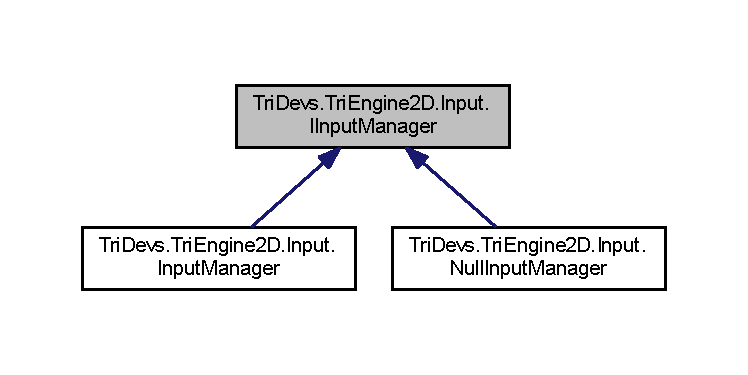
\includegraphics[width=350pt]{interface_tri_devs_1_1_tri_engine2_d_1_1_input_1_1_i_input_manager__inherit__graph}
\end{center}
\end{figure}
\subsection*{Public Member Functions}
\begin{DoxyCompactItemize}
\item 
void \hyperlink{interface_tri_devs_1_1_tri_engine2_d_1_1_input_1_1_i_input_manager_a0cc046decb859d0f4d0b23a5a83d078f}{Update} ()
\begin{DoxyCompactList}\small\item\em Updates the input manager, refreshing all current and previous states. \end{DoxyCompactList}\item 
bool \hyperlink{interface_tri_devs_1_1_tri_engine2_d_1_1_input_1_1_i_input_manager_a38249eb3d1b1df7bb13835863829e8ab}{Is\-Key\-Up} (Key key)
\begin{DoxyCompactList}\small\item\em Returns whether or not the specified key is currently unpressed. \end{DoxyCompactList}\item 
bool \hyperlink{interface_tri_devs_1_1_tri_engine2_d_1_1_input_1_1_i_input_manager_a9f7767fe300acc7861be1e0c94ba415b}{Is\-Key\-Down} (Key key)
\begin{DoxyCompactList}\small\item\em Returns whether or not the specified key is currently being pressed. \end{DoxyCompactList}\item 
bool \hyperlink{interface_tri_devs_1_1_tri_engine2_d_1_1_input_1_1_i_input_manager_a0dcc608b0c3ffb806262c9f829373dcb}{Key\-Pressed} (Key key)
\begin{DoxyCompactList}\small\item\em Returns whether or not the specified key has been pressed. \end{DoxyCompactList}\item 
bool \hyperlink{interface_tri_devs_1_1_tri_engine2_d_1_1_input_1_1_i_input_manager_a54feb5f23a217ad5bcd104cc8912247b}{Key\-Released} (Key key)
\begin{DoxyCompactList}\small\item\em Returns whether or not the specified key has been released. \end{DoxyCompactList}\item 
bool \hyperlink{interface_tri_devs_1_1_tri_engine2_d_1_1_input_1_1_i_input_manager_a40407fe8d40fe3016c9d086dd4917be4}{Is\-Mouse\-Up} (Mouse\-Button button)
\begin{DoxyCompactList}\small\item\em Returns whether or not the specified mouse button is currently unpressed. \end{DoxyCompactList}\item 
bool \hyperlink{interface_tri_devs_1_1_tri_engine2_d_1_1_input_1_1_i_input_manager_aa6a017570fcda20760b7e491b8351574}{Is\-Mouse\-Down} (Mouse\-Button button)
\begin{DoxyCompactList}\small\item\em Returns whether or not the specified mouse button is currently being pressed. \end{DoxyCompactList}\item 
bool \hyperlink{interface_tri_devs_1_1_tri_engine2_d_1_1_input_1_1_i_input_manager_a83a14eebbb3a994cdb1a2dfcf387b4cb}{Mouse\-Pressed} (Mouse\-Button button)
\begin{DoxyCompactList}\small\item\em Returns whether or not the specified mouse button has been pressed. \end{DoxyCompactList}\item 
bool \hyperlink{interface_tri_devs_1_1_tri_engine2_d_1_1_input_1_1_i_input_manager_ad73037492d302fb465532f4000b76478}{Mouse\-Released} (Mouse\-Button button)
\begin{DoxyCompactList}\small\item\em Returns whether or not the specified mouse button has been released. \end{DoxyCompactList}\item 
bool \hyperlink{interface_tri_devs_1_1_tri_engine2_d_1_1_input_1_1_i_input_manager_a0d298286b93f065e054a2d3e9fdc4073}{Is\-Wheel\-Up} ()
\begin{DoxyCompactList}\small\item\em Returns whether the mouse wheel was scrolled up. \end{DoxyCompactList}\item 
bool \hyperlink{interface_tri_devs_1_1_tri_engine2_d_1_1_input_1_1_i_input_manager_a01e7bb0f8255bb071678e7bcb86b97a3}{Is\-Wheel\-Down} ()
\begin{DoxyCompactList}\small\item\em Returns whether the mouse wheel was scrolled down. \end{DoxyCompactList}\item 
bool \hyperlink{interface_tri_devs_1_1_tri_engine2_d_1_1_input_1_1_i_input_manager_af7aeda5d94a3dc5e60384e4a62f84fd2}{Is\-Wheel\-Changed} ()
\begin{DoxyCompactList}\small\item\em Returns whether the mouse wheel scrolled at all. \end{DoxyCompactList}\item 
int \hyperlink{interface_tri_devs_1_1_tri_engine2_d_1_1_input_1_1_i_input_manager_afbd3f200724d419be432da3a2dc639bd}{Wheel\-Change} ()
\begin{DoxyCompactList}\small\item\em Returns the mouse wheel's change in value. \end{DoxyCompactList}\end{DoxyCompactItemize}
\subsection*{Properties}
\begin{DoxyCompactItemize}
\item 
int \hyperlink{interface_tri_devs_1_1_tri_engine2_d_1_1_input_1_1_i_input_manager_a545e03fc7c5084bcf00f018145625c19}{Mouse\-X}\hspace{0.3cm}{\ttfamily  \mbox{[}get\mbox{]}}
\begin{DoxyCompactList}\small\item\em Gets the absolute X position of the pointer, in window pixel coordinates. \end{DoxyCompactList}\item 
int \hyperlink{interface_tri_devs_1_1_tri_engine2_d_1_1_input_1_1_i_input_manager_a143f5147279fe1807635d1e8b9b4e7c7}{Mouse\-Y}\hspace{0.3cm}{\ttfamily  \mbox{[}get\mbox{]}}
\begin{DoxyCompactList}\small\item\em Gets the absolute Y position of the pointer, in window pixel coordinates. \end{DoxyCompactList}\item 
Point$<$ int $>$ \hyperlink{interface_tri_devs_1_1_tri_engine2_d_1_1_input_1_1_i_input_manager_a1c7099f4027c14a36873ca2809ecdb62}{Mouse\-Position}\hspace{0.3cm}{\ttfamily  \mbox{[}get\mbox{]}}
\begin{DoxyCompactList}\small\item\em Gets a Point representing the position of the mouse pointer, in window pixel coordinates. \end{DoxyCompactList}\item 
int \hyperlink{interface_tri_devs_1_1_tri_engine2_d_1_1_input_1_1_i_input_manager_a7d42befc637abbaf51f46ba93d12aff8}{Mouse\-Wheel\-Value}\hspace{0.3cm}{\ttfamily  \mbox{[}get\mbox{]}}
\begin{DoxyCompactList}\small\item\em Gets the current value of the mouse wheel. \end{DoxyCompactList}\item 
bool \hyperlink{interface_tri_devs_1_1_tri_engine2_d_1_1_input_1_1_i_input_manager_a4864942443d3939d630504c7da9fbfd6}{this\mbox{[}\-Key key\mbox{]}}\hspace{0.3cm}{\ttfamily  \mbox{[}get\mbox{]}}
\begin{DoxyCompactList}\small\item\em Gets a boolean value indicating whether the specified Open\-T\-K.\-Input.\-Key is pressed. \end{DoxyCompactList}\item 
bool \hyperlink{interface_tri_devs_1_1_tri_engine2_d_1_1_input_1_1_i_input_manager_a1ab67e0dc3518f968641893310d47db1}{this\mbox{[}\-Mouse\-Button button\mbox{]}}\hspace{0.3cm}{\ttfamily  \mbox{[}get\mbox{]}}
\begin{DoxyCompactList}\small\item\em Gets a boolean value indicating whether the specified Open\-T\-K.\-Input.\-Mouse\-Button is pressed. \end{DoxyCompactList}\end{DoxyCompactItemize}
\subsection*{Events}
\begin{DoxyCompactItemize}
\item 
Key\-Down\-Event\-Handler \hyperlink{interface_tri_devs_1_1_tri_engine2_d_1_1_input_1_1_i_input_manager_a5948602f547dc681864f39def0808154}{Key\-Down}
\begin{DoxyCompactList}\small\item\em Raised when a key is pressed down. \end{DoxyCompactList}\item 
Key\-Up\-Event\-Handler \hyperlink{interface_tri_devs_1_1_tri_engine2_d_1_1_input_1_1_i_input_manager_a84ffeb24cb3583038b62b4a91fcfadc4}{Key\-Up}
\begin{DoxyCompactList}\small\item\em Raised when a key is released. \end{DoxyCompactList}\item 
Key\-Press\-Event\-Handler \hyperlink{interface_tri_devs_1_1_tri_engine2_d_1_1_input_1_1_i_input_manager_a08f324d5224dd4f6b2214f9b5ea76c22}{Key\-Press}
\begin{DoxyCompactList}\small\item\em Raised when a character is typed. \end{DoxyCompactList}\item 
Mouse\-Down\-Event\-Handler \hyperlink{interface_tri_devs_1_1_tri_engine2_d_1_1_input_1_1_i_input_manager_a5bf6aff053702524922cdef1c0eda2f6}{Mouse\-Down}
\begin{DoxyCompactList}\small\item\em Raised when a mouse button is pressed down. \end{DoxyCompactList}\item 
Mouse\-Up\-Event\-Handler \hyperlink{interface_tri_devs_1_1_tri_engine2_d_1_1_input_1_1_i_input_manager_afbaf9eee227f333070ed9ff2c42a40c7}{Mouse\-Up}
\begin{DoxyCompactList}\small\item\em Raised when a mouse button is released. \end{DoxyCompactList}\item 
Mouse\-Wheel\-Changed\-Event\-Handler \hyperlink{interface_tri_devs_1_1_tri_engine2_d_1_1_input_1_1_i_input_manager_ac560db0d881cbf110f713f5791e187ed}{Wheel\-Changed}
\begin{DoxyCompactList}\small\item\em Raised when the mouse wheel value changes. \end{DoxyCompactList}\item 
Mouse\-Wheel\-Down\-Event\-Handler \hyperlink{interface_tri_devs_1_1_tri_engine2_d_1_1_input_1_1_i_input_manager_a8022b6f3d57b2e0acfa56af4d71099f9}{Wheel\-Down}
\begin{DoxyCompactList}\small\item\em Raised when the mouse wheel is scrolled downwards. \end{DoxyCompactList}\item 
Mouse\-Wheel\-Up\-Event\-Handler \hyperlink{interface_tri_devs_1_1_tri_engine2_d_1_1_input_1_1_i_input_manager_ad1537ccd8ae47fbfa29fb1ae44da8cb4}{Wheel\-Up}
\begin{DoxyCompactList}\small\item\em Raised when the mouse wheel is scrolled upwards. \end{DoxyCompactList}\end{DoxyCompactItemize}


\subsection{Detailed Description}
Provides various methods to query input devices like the keyboard. 



\subsection{Member Function Documentation}
\hypertarget{interface_tri_devs_1_1_tri_engine2_d_1_1_input_1_1_i_input_manager_a9f7767fe300acc7861be1e0c94ba415b}{\index{Tri\-Devs\-::\-Tri\-Engine2\-D\-::\-Input\-::\-I\-Input\-Manager@{Tri\-Devs\-::\-Tri\-Engine2\-D\-::\-Input\-::\-I\-Input\-Manager}!Is\-Key\-Down@{Is\-Key\-Down}}
\index{Is\-Key\-Down@{Is\-Key\-Down}!TriDevs::TriEngine2D::Input::IInputManager@{Tri\-Devs\-::\-Tri\-Engine2\-D\-::\-Input\-::\-I\-Input\-Manager}}
\subsubsection[{Is\-Key\-Down}]{\setlength{\rightskip}{0pt plus 5cm}bool Tri\-Devs.\-Tri\-Engine2\-D.\-Input.\-I\-Input\-Manager.\-Is\-Key\-Down (
\begin{DoxyParamCaption}
\item[{Key}]{key}
\end{DoxyParamCaption}
)}}\label{interface_tri_devs_1_1_tri_engine2_d_1_1_input_1_1_i_input_manager_a9f7767fe300acc7861be1e0c94ba415b}


Returns whether or not the specified key is currently being pressed. 


\begin{DoxyParams}{Parameters}
{\em key} & Key to query for.\\
\hline
\end{DoxyParams}
\begin{DoxyReturn}{Returns}
True if key is currently being pressed, false otherwise.
\end{DoxyReturn}


Implemented in \hyperlink{class_tri_devs_1_1_tri_engine2_d_1_1_input_1_1_input_manager_a22a6938da450c2606ea779e980a33dbb}{Tri\-Devs.\-Tri\-Engine2\-D.\-Input.\-Input\-Manager}, and \hyperlink{class_tri_devs_1_1_tri_engine2_d_1_1_input_1_1_null_input_manager_a638ccbbaebcc111ae54943f229e887d6}{Tri\-Devs.\-Tri\-Engine2\-D.\-Input.\-Null\-Input\-Manager}.

\hypertarget{interface_tri_devs_1_1_tri_engine2_d_1_1_input_1_1_i_input_manager_a38249eb3d1b1df7bb13835863829e8ab}{\index{Tri\-Devs\-::\-Tri\-Engine2\-D\-::\-Input\-::\-I\-Input\-Manager@{Tri\-Devs\-::\-Tri\-Engine2\-D\-::\-Input\-::\-I\-Input\-Manager}!Is\-Key\-Up@{Is\-Key\-Up}}
\index{Is\-Key\-Up@{Is\-Key\-Up}!TriDevs::TriEngine2D::Input::IInputManager@{Tri\-Devs\-::\-Tri\-Engine2\-D\-::\-Input\-::\-I\-Input\-Manager}}
\subsubsection[{Is\-Key\-Up}]{\setlength{\rightskip}{0pt plus 5cm}bool Tri\-Devs.\-Tri\-Engine2\-D.\-Input.\-I\-Input\-Manager.\-Is\-Key\-Up (
\begin{DoxyParamCaption}
\item[{Key}]{key}
\end{DoxyParamCaption}
)}}\label{interface_tri_devs_1_1_tri_engine2_d_1_1_input_1_1_i_input_manager_a38249eb3d1b1df7bb13835863829e8ab}


Returns whether or not the specified key is currently unpressed. 


\begin{DoxyParams}{Parameters}
{\em key} & Key to query for.\\
\hline
\end{DoxyParams}
\begin{DoxyReturn}{Returns}
True if the key is currently up (not pressed), false otherwise.
\end{DoxyReturn}


Implemented in \hyperlink{class_tri_devs_1_1_tri_engine2_d_1_1_input_1_1_input_manager_a158e8ca55c8c2f972c791204cbac1b06}{Tri\-Devs.\-Tri\-Engine2\-D.\-Input.\-Input\-Manager}, and \hyperlink{class_tri_devs_1_1_tri_engine2_d_1_1_input_1_1_null_input_manager_ad3bd61fe68f86ea69f4c1c84eb4782ef}{Tri\-Devs.\-Tri\-Engine2\-D.\-Input.\-Null\-Input\-Manager}.

\hypertarget{interface_tri_devs_1_1_tri_engine2_d_1_1_input_1_1_i_input_manager_aa6a017570fcda20760b7e491b8351574}{\index{Tri\-Devs\-::\-Tri\-Engine2\-D\-::\-Input\-::\-I\-Input\-Manager@{Tri\-Devs\-::\-Tri\-Engine2\-D\-::\-Input\-::\-I\-Input\-Manager}!Is\-Mouse\-Down@{Is\-Mouse\-Down}}
\index{Is\-Mouse\-Down@{Is\-Mouse\-Down}!TriDevs::TriEngine2D::Input::IInputManager@{Tri\-Devs\-::\-Tri\-Engine2\-D\-::\-Input\-::\-I\-Input\-Manager}}
\subsubsection[{Is\-Mouse\-Down}]{\setlength{\rightskip}{0pt plus 5cm}bool Tri\-Devs.\-Tri\-Engine2\-D.\-Input.\-I\-Input\-Manager.\-Is\-Mouse\-Down (
\begin{DoxyParamCaption}
\item[{Mouse\-Button}]{button}
\end{DoxyParamCaption}
)}}\label{interface_tri_devs_1_1_tri_engine2_d_1_1_input_1_1_i_input_manager_aa6a017570fcda20760b7e491b8351574}


Returns whether or not the specified mouse button is currently being pressed. 


\begin{DoxyParams}{Parameters}
{\em button} & The button to query for.\\
\hline
\end{DoxyParams}
\begin{DoxyReturn}{Returns}
True if button is currently being pressed, false otherwise.
\end{DoxyReturn}


Implemented in \hyperlink{class_tri_devs_1_1_tri_engine2_d_1_1_input_1_1_input_manager_a6a26c5121fad6a3eefcf552a980c6ff3}{Tri\-Devs.\-Tri\-Engine2\-D.\-Input.\-Input\-Manager}, and \hyperlink{class_tri_devs_1_1_tri_engine2_d_1_1_input_1_1_null_input_manager_a951f1aff66e48b3634938a78d7b0c309}{Tri\-Devs.\-Tri\-Engine2\-D.\-Input.\-Null\-Input\-Manager}.

\hypertarget{interface_tri_devs_1_1_tri_engine2_d_1_1_input_1_1_i_input_manager_a40407fe8d40fe3016c9d086dd4917be4}{\index{Tri\-Devs\-::\-Tri\-Engine2\-D\-::\-Input\-::\-I\-Input\-Manager@{Tri\-Devs\-::\-Tri\-Engine2\-D\-::\-Input\-::\-I\-Input\-Manager}!Is\-Mouse\-Up@{Is\-Mouse\-Up}}
\index{Is\-Mouse\-Up@{Is\-Mouse\-Up}!TriDevs::TriEngine2D::Input::IInputManager@{Tri\-Devs\-::\-Tri\-Engine2\-D\-::\-Input\-::\-I\-Input\-Manager}}
\subsubsection[{Is\-Mouse\-Up}]{\setlength{\rightskip}{0pt plus 5cm}bool Tri\-Devs.\-Tri\-Engine2\-D.\-Input.\-I\-Input\-Manager.\-Is\-Mouse\-Up (
\begin{DoxyParamCaption}
\item[{Mouse\-Button}]{button}
\end{DoxyParamCaption}
)}}\label{interface_tri_devs_1_1_tri_engine2_d_1_1_input_1_1_i_input_manager_a40407fe8d40fe3016c9d086dd4917be4}


Returns whether or not the specified mouse button is currently unpressed. 


\begin{DoxyParams}{Parameters}
{\em button} & Button to query for.\\
\hline
\end{DoxyParams}
\begin{DoxyReturn}{Returns}
True if the button is currently up (not pressed), false otherwise.
\end{DoxyReturn}


Implemented in \hyperlink{class_tri_devs_1_1_tri_engine2_d_1_1_input_1_1_input_manager_a2d554c09767cc9f36b21f5bcde4cefa3}{Tri\-Devs.\-Tri\-Engine2\-D.\-Input.\-Input\-Manager}, and \hyperlink{class_tri_devs_1_1_tri_engine2_d_1_1_input_1_1_null_input_manager_aaa1e94165672415d9f4c96f4b746195f}{Tri\-Devs.\-Tri\-Engine2\-D.\-Input.\-Null\-Input\-Manager}.

\hypertarget{interface_tri_devs_1_1_tri_engine2_d_1_1_input_1_1_i_input_manager_af7aeda5d94a3dc5e60384e4a62f84fd2}{\index{Tri\-Devs\-::\-Tri\-Engine2\-D\-::\-Input\-::\-I\-Input\-Manager@{Tri\-Devs\-::\-Tri\-Engine2\-D\-::\-Input\-::\-I\-Input\-Manager}!Is\-Wheel\-Changed@{Is\-Wheel\-Changed}}
\index{Is\-Wheel\-Changed@{Is\-Wheel\-Changed}!TriDevs::TriEngine2D::Input::IInputManager@{Tri\-Devs\-::\-Tri\-Engine2\-D\-::\-Input\-::\-I\-Input\-Manager}}
\subsubsection[{Is\-Wheel\-Changed}]{\setlength{\rightskip}{0pt plus 5cm}bool Tri\-Devs.\-Tri\-Engine2\-D.\-Input.\-I\-Input\-Manager.\-Is\-Wheel\-Changed (
\begin{DoxyParamCaption}
{}
\end{DoxyParamCaption}
)}}\label{interface_tri_devs_1_1_tri_engine2_d_1_1_input_1_1_i_input_manager_af7aeda5d94a3dc5e60384e4a62f84fd2}


Returns whether the mouse wheel scrolled at all. 

\begin{DoxyReturn}{Returns}
True if the mouse wheel scrolled, false otherwise.
\end{DoxyReturn}


Implemented in \hyperlink{class_tri_devs_1_1_tri_engine2_d_1_1_input_1_1_input_manager_a246df48ba2c2d15aba537f19abb806da}{Tri\-Devs.\-Tri\-Engine2\-D.\-Input.\-Input\-Manager}, and \hyperlink{class_tri_devs_1_1_tri_engine2_d_1_1_input_1_1_null_input_manager_afc121c18682c20aba9cb9f224c2a907f}{Tri\-Devs.\-Tri\-Engine2\-D.\-Input.\-Null\-Input\-Manager}.

\hypertarget{interface_tri_devs_1_1_tri_engine2_d_1_1_input_1_1_i_input_manager_a01e7bb0f8255bb071678e7bcb86b97a3}{\index{Tri\-Devs\-::\-Tri\-Engine2\-D\-::\-Input\-::\-I\-Input\-Manager@{Tri\-Devs\-::\-Tri\-Engine2\-D\-::\-Input\-::\-I\-Input\-Manager}!Is\-Wheel\-Down@{Is\-Wheel\-Down}}
\index{Is\-Wheel\-Down@{Is\-Wheel\-Down}!TriDevs::TriEngine2D::Input::IInputManager@{Tri\-Devs\-::\-Tri\-Engine2\-D\-::\-Input\-::\-I\-Input\-Manager}}
\subsubsection[{Is\-Wheel\-Down}]{\setlength{\rightskip}{0pt plus 5cm}bool Tri\-Devs.\-Tri\-Engine2\-D.\-Input.\-I\-Input\-Manager.\-Is\-Wheel\-Down (
\begin{DoxyParamCaption}
{}
\end{DoxyParamCaption}
)}}\label{interface_tri_devs_1_1_tri_engine2_d_1_1_input_1_1_i_input_manager_a01e7bb0f8255bb071678e7bcb86b97a3}


Returns whether the mouse wheel was scrolled down. 

\begin{DoxyReturn}{Returns}
True if mouse wheel was scrolled down, false otherwise.
\end{DoxyReturn}


Implemented in \hyperlink{class_tri_devs_1_1_tri_engine2_d_1_1_input_1_1_input_manager_a3d5c73853f0df96af5d76584bea512b2}{Tri\-Devs.\-Tri\-Engine2\-D.\-Input.\-Input\-Manager}, and \hyperlink{class_tri_devs_1_1_tri_engine2_d_1_1_input_1_1_null_input_manager_ae9e8a97e2232df463ef38f6020500a34}{Tri\-Devs.\-Tri\-Engine2\-D.\-Input.\-Null\-Input\-Manager}.

\hypertarget{interface_tri_devs_1_1_tri_engine2_d_1_1_input_1_1_i_input_manager_a0d298286b93f065e054a2d3e9fdc4073}{\index{Tri\-Devs\-::\-Tri\-Engine2\-D\-::\-Input\-::\-I\-Input\-Manager@{Tri\-Devs\-::\-Tri\-Engine2\-D\-::\-Input\-::\-I\-Input\-Manager}!Is\-Wheel\-Up@{Is\-Wheel\-Up}}
\index{Is\-Wheel\-Up@{Is\-Wheel\-Up}!TriDevs::TriEngine2D::Input::IInputManager@{Tri\-Devs\-::\-Tri\-Engine2\-D\-::\-Input\-::\-I\-Input\-Manager}}
\subsubsection[{Is\-Wheel\-Up}]{\setlength{\rightskip}{0pt plus 5cm}bool Tri\-Devs.\-Tri\-Engine2\-D.\-Input.\-I\-Input\-Manager.\-Is\-Wheel\-Up (
\begin{DoxyParamCaption}
{}
\end{DoxyParamCaption}
)}}\label{interface_tri_devs_1_1_tri_engine2_d_1_1_input_1_1_i_input_manager_a0d298286b93f065e054a2d3e9fdc4073}


Returns whether the mouse wheel was scrolled up. 

\begin{DoxyReturn}{Returns}
True if mouse wheel was scrolled up, false otherwise.
\end{DoxyReturn}


Implemented in \hyperlink{class_tri_devs_1_1_tri_engine2_d_1_1_input_1_1_input_manager_aa4d5c302876f5e4f99bbca7381f3d58b}{Tri\-Devs.\-Tri\-Engine2\-D.\-Input.\-Input\-Manager}, and \hyperlink{class_tri_devs_1_1_tri_engine2_d_1_1_input_1_1_null_input_manager_a1e813af823111332d09bfdacc545a929}{Tri\-Devs.\-Tri\-Engine2\-D.\-Input.\-Null\-Input\-Manager}.

\hypertarget{interface_tri_devs_1_1_tri_engine2_d_1_1_input_1_1_i_input_manager_a0dcc608b0c3ffb806262c9f829373dcb}{\index{Tri\-Devs\-::\-Tri\-Engine2\-D\-::\-Input\-::\-I\-Input\-Manager@{Tri\-Devs\-::\-Tri\-Engine2\-D\-::\-Input\-::\-I\-Input\-Manager}!Key\-Pressed@{Key\-Pressed}}
\index{Key\-Pressed@{Key\-Pressed}!TriDevs::TriEngine2D::Input::IInputManager@{Tri\-Devs\-::\-Tri\-Engine2\-D\-::\-Input\-::\-I\-Input\-Manager}}
\subsubsection[{Key\-Pressed}]{\setlength{\rightskip}{0pt plus 5cm}bool Tri\-Devs.\-Tri\-Engine2\-D.\-Input.\-I\-Input\-Manager.\-Key\-Pressed (
\begin{DoxyParamCaption}
\item[{Key}]{key}
\end{DoxyParamCaption}
)}}\label{interface_tri_devs_1_1_tri_engine2_d_1_1_input_1_1_i_input_manager_a0dcc608b0c3ffb806262c9f829373dcb}


Returns whether or not the specified key has been pressed. 

Only returns true if the last state of the key was not pressed. 


\begin{DoxyParams}{Parameters}
{\em key} & Key to query for.\\
\hline
\end{DoxyParams}
\begin{DoxyReturn}{Returns}
True if key was pressed, false otherwise.
\end{DoxyReturn}


Implemented in \hyperlink{class_tri_devs_1_1_tri_engine2_d_1_1_input_1_1_input_manager_ab3a260ea268b4683596ff5a244fd2d95}{Tri\-Devs.\-Tri\-Engine2\-D.\-Input.\-Input\-Manager}, and \hyperlink{class_tri_devs_1_1_tri_engine2_d_1_1_input_1_1_null_input_manager_a2de0da3893be579c99690caa0d3cd2cc}{Tri\-Devs.\-Tri\-Engine2\-D.\-Input.\-Null\-Input\-Manager}.

\hypertarget{interface_tri_devs_1_1_tri_engine2_d_1_1_input_1_1_i_input_manager_a54feb5f23a217ad5bcd104cc8912247b}{\index{Tri\-Devs\-::\-Tri\-Engine2\-D\-::\-Input\-::\-I\-Input\-Manager@{Tri\-Devs\-::\-Tri\-Engine2\-D\-::\-Input\-::\-I\-Input\-Manager}!Key\-Released@{Key\-Released}}
\index{Key\-Released@{Key\-Released}!TriDevs::TriEngine2D::Input::IInputManager@{Tri\-Devs\-::\-Tri\-Engine2\-D\-::\-Input\-::\-I\-Input\-Manager}}
\subsubsection[{Key\-Released}]{\setlength{\rightskip}{0pt plus 5cm}bool Tri\-Devs.\-Tri\-Engine2\-D.\-Input.\-I\-Input\-Manager.\-Key\-Released (
\begin{DoxyParamCaption}
\item[{Key}]{key}
\end{DoxyParamCaption}
)}}\label{interface_tri_devs_1_1_tri_engine2_d_1_1_input_1_1_i_input_manager_a54feb5f23a217ad5bcd104cc8912247b}


Returns whether or not the specified key has been released. 

Only returns true if the last state of the key was pressed. 


\begin{DoxyParams}{Parameters}
{\em key} & Key to query for.\\
\hline
\end{DoxyParams}
\begin{DoxyReturn}{Returns}
True if key was released, false otherwise.
\end{DoxyReturn}


Implemented in \hyperlink{class_tri_devs_1_1_tri_engine2_d_1_1_input_1_1_input_manager_a1e74615e2ccde33e98d262d3c48d729a}{Tri\-Devs.\-Tri\-Engine2\-D.\-Input.\-Input\-Manager}, and \hyperlink{class_tri_devs_1_1_tri_engine2_d_1_1_input_1_1_null_input_manager_aadf04bc0e73da9612c1cdd435fdb6867}{Tri\-Devs.\-Tri\-Engine2\-D.\-Input.\-Null\-Input\-Manager}.

\hypertarget{interface_tri_devs_1_1_tri_engine2_d_1_1_input_1_1_i_input_manager_a83a14eebbb3a994cdb1a2dfcf387b4cb}{\index{Tri\-Devs\-::\-Tri\-Engine2\-D\-::\-Input\-::\-I\-Input\-Manager@{Tri\-Devs\-::\-Tri\-Engine2\-D\-::\-Input\-::\-I\-Input\-Manager}!Mouse\-Pressed@{Mouse\-Pressed}}
\index{Mouse\-Pressed@{Mouse\-Pressed}!TriDevs::TriEngine2D::Input::IInputManager@{Tri\-Devs\-::\-Tri\-Engine2\-D\-::\-Input\-::\-I\-Input\-Manager}}
\subsubsection[{Mouse\-Pressed}]{\setlength{\rightskip}{0pt plus 5cm}bool Tri\-Devs.\-Tri\-Engine2\-D.\-Input.\-I\-Input\-Manager.\-Mouse\-Pressed (
\begin{DoxyParamCaption}
\item[{Mouse\-Button}]{button}
\end{DoxyParamCaption}
)}}\label{interface_tri_devs_1_1_tri_engine2_d_1_1_input_1_1_i_input_manager_a83a14eebbb3a994cdb1a2dfcf387b4cb}


Returns whether or not the specified mouse button has been pressed. 

Only returns true if the last state of the mouse button was not pressed. 


\begin{DoxyParams}{Parameters}
{\em button} & Button to query for.\\
\hline
\end{DoxyParams}
\begin{DoxyReturn}{Returns}
True if button was pressed, false otherwise.
\end{DoxyReturn}


Implemented in \hyperlink{class_tri_devs_1_1_tri_engine2_d_1_1_input_1_1_input_manager_a114492d5a852be9f58b3971511af3c09}{Tri\-Devs.\-Tri\-Engine2\-D.\-Input.\-Input\-Manager}, and \hyperlink{class_tri_devs_1_1_tri_engine2_d_1_1_input_1_1_null_input_manager_a2d18f7c8321263f0af91ac253ab4fc26}{Tri\-Devs.\-Tri\-Engine2\-D.\-Input.\-Null\-Input\-Manager}.

\hypertarget{interface_tri_devs_1_1_tri_engine2_d_1_1_input_1_1_i_input_manager_ad73037492d302fb465532f4000b76478}{\index{Tri\-Devs\-::\-Tri\-Engine2\-D\-::\-Input\-::\-I\-Input\-Manager@{Tri\-Devs\-::\-Tri\-Engine2\-D\-::\-Input\-::\-I\-Input\-Manager}!Mouse\-Released@{Mouse\-Released}}
\index{Mouse\-Released@{Mouse\-Released}!TriDevs::TriEngine2D::Input::IInputManager@{Tri\-Devs\-::\-Tri\-Engine2\-D\-::\-Input\-::\-I\-Input\-Manager}}
\subsubsection[{Mouse\-Released}]{\setlength{\rightskip}{0pt plus 5cm}bool Tri\-Devs.\-Tri\-Engine2\-D.\-Input.\-I\-Input\-Manager.\-Mouse\-Released (
\begin{DoxyParamCaption}
\item[{Mouse\-Button}]{button}
\end{DoxyParamCaption}
)}}\label{interface_tri_devs_1_1_tri_engine2_d_1_1_input_1_1_i_input_manager_ad73037492d302fb465532f4000b76478}


Returns whether or not the specified mouse button has been released. 

Only returns true if the last state of the button was pressed. 


\begin{DoxyParams}{Parameters}
{\em button} & The button to query for.\\
\hline
\end{DoxyParams}
\begin{DoxyReturn}{Returns}
True if the button was released, false otherwise.
\end{DoxyReturn}


Implemented in \hyperlink{class_tri_devs_1_1_tri_engine2_d_1_1_input_1_1_input_manager_aee465cfdff75ddcf53cd62aa38c09013}{Tri\-Devs.\-Tri\-Engine2\-D.\-Input.\-Input\-Manager}, and \hyperlink{class_tri_devs_1_1_tri_engine2_d_1_1_input_1_1_null_input_manager_a89dd9c15a7ff89303e9130797fc8a835}{Tri\-Devs.\-Tri\-Engine2\-D.\-Input.\-Null\-Input\-Manager}.

\hypertarget{interface_tri_devs_1_1_tri_engine2_d_1_1_input_1_1_i_input_manager_a0cc046decb859d0f4d0b23a5a83d078f}{\index{Tri\-Devs\-::\-Tri\-Engine2\-D\-::\-Input\-::\-I\-Input\-Manager@{Tri\-Devs\-::\-Tri\-Engine2\-D\-::\-Input\-::\-I\-Input\-Manager}!Update@{Update}}
\index{Update@{Update}!TriDevs::TriEngine2D::Input::IInputManager@{Tri\-Devs\-::\-Tri\-Engine2\-D\-::\-Input\-::\-I\-Input\-Manager}}
\subsubsection[{Update}]{\setlength{\rightskip}{0pt plus 5cm}void Tri\-Devs.\-Tri\-Engine2\-D.\-Input.\-I\-Input\-Manager.\-Update (
\begin{DoxyParamCaption}
{}
\end{DoxyParamCaption}
)}}\label{interface_tri_devs_1_1_tri_engine2_d_1_1_input_1_1_i_input_manager_a0cc046decb859d0f4d0b23a5a83d078f}


Updates the input manager, refreshing all current and previous states. 



Implemented in \hyperlink{class_tri_devs_1_1_tri_engine2_d_1_1_input_1_1_input_manager_a5ef0bd64a85fdafc34324cf231038302}{Tri\-Devs.\-Tri\-Engine2\-D.\-Input.\-Input\-Manager}, and \hyperlink{class_tri_devs_1_1_tri_engine2_d_1_1_input_1_1_null_input_manager_a7713c34aa9dea7d6f0878e9c99217df3}{Tri\-Devs.\-Tri\-Engine2\-D.\-Input.\-Null\-Input\-Manager}.

\hypertarget{interface_tri_devs_1_1_tri_engine2_d_1_1_input_1_1_i_input_manager_afbd3f200724d419be432da3a2dc639bd}{\index{Tri\-Devs\-::\-Tri\-Engine2\-D\-::\-Input\-::\-I\-Input\-Manager@{Tri\-Devs\-::\-Tri\-Engine2\-D\-::\-Input\-::\-I\-Input\-Manager}!Wheel\-Change@{Wheel\-Change}}
\index{Wheel\-Change@{Wheel\-Change}!TriDevs::TriEngine2D::Input::IInputManager@{Tri\-Devs\-::\-Tri\-Engine2\-D\-::\-Input\-::\-I\-Input\-Manager}}
\subsubsection[{Wheel\-Change}]{\setlength{\rightskip}{0pt plus 5cm}int Tri\-Devs.\-Tri\-Engine2\-D.\-Input.\-I\-Input\-Manager.\-Wheel\-Change (
\begin{DoxyParamCaption}
{}
\end{DoxyParamCaption}
)}}\label{interface_tri_devs_1_1_tri_engine2_d_1_1_input_1_1_i_input_manager_afbd3f200724d419be432da3a2dc639bd}


Returns the mouse wheel's change in value. 

\begin{DoxyReturn}{Returns}
Negative value if wheel scrolled down, positive value if scrolled up, zero if not scrolled.
\end{DoxyReturn}


Implemented in \hyperlink{class_tri_devs_1_1_tri_engine2_d_1_1_input_1_1_input_manager_af8aa353e5d9434776181a42312c1499b}{Tri\-Devs.\-Tri\-Engine2\-D.\-Input.\-Input\-Manager}, and \hyperlink{class_tri_devs_1_1_tri_engine2_d_1_1_input_1_1_null_input_manager_a48b6584ca2a845d0ae108a0e08145c43}{Tri\-Devs.\-Tri\-Engine2\-D.\-Input.\-Null\-Input\-Manager}.



\subsection{Property Documentation}
\hypertarget{interface_tri_devs_1_1_tri_engine2_d_1_1_input_1_1_i_input_manager_a1c7099f4027c14a36873ca2809ecdb62}{\index{Tri\-Devs\-::\-Tri\-Engine2\-D\-::\-Input\-::\-I\-Input\-Manager@{Tri\-Devs\-::\-Tri\-Engine2\-D\-::\-Input\-::\-I\-Input\-Manager}!Mouse\-Position@{Mouse\-Position}}
\index{Mouse\-Position@{Mouse\-Position}!TriDevs::TriEngine2D::Input::IInputManager@{Tri\-Devs\-::\-Tri\-Engine2\-D\-::\-Input\-::\-I\-Input\-Manager}}
\subsubsection[{Mouse\-Position}]{\setlength{\rightskip}{0pt plus 5cm}Point$<$int$>$ Tri\-Devs.\-Tri\-Engine2\-D.\-Input.\-I\-Input\-Manager.\-Mouse\-Position\hspace{0.3cm}{\ttfamily [get]}}}\label{interface_tri_devs_1_1_tri_engine2_d_1_1_input_1_1_i_input_manager_a1c7099f4027c14a36873ca2809ecdb62}


Gets a Point representing the position of the mouse pointer, in window pixel coordinates. 

\hypertarget{interface_tri_devs_1_1_tri_engine2_d_1_1_input_1_1_i_input_manager_a7d42befc637abbaf51f46ba93d12aff8}{\index{Tri\-Devs\-::\-Tri\-Engine2\-D\-::\-Input\-::\-I\-Input\-Manager@{Tri\-Devs\-::\-Tri\-Engine2\-D\-::\-Input\-::\-I\-Input\-Manager}!Mouse\-Wheel\-Value@{Mouse\-Wheel\-Value}}
\index{Mouse\-Wheel\-Value@{Mouse\-Wheel\-Value}!TriDevs::TriEngine2D::Input::IInputManager@{Tri\-Devs\-::\-Tri\-Engine2\-D\-::\-Input\-::\-I\-Input\-Manager}}
\subsubsection[{Mouse\-Wheel\-Value}]{\setlength{\rightskip}{0pt plus 5cm}int Tri\-Devs.\-Tri\-Engine2\-D.\-Input.\-I\-Input\-Manager.\-Mouse\-Wheel\-Value\hspace{0.3cm}{\ttfamily [get]}}}\label{interface_tri_devs_1_1_tri_engine2_d_1_1_input_1_1_i_input_manager_a7d42befc637abbaf51f46ba93d12aff8}


Gets the current value of the mouse wheel. 

\hypertarget{interface_tri_devs_1_1_tri_engine2_d_1_1_input_1_1_i_input_manager_a545e03fc7c5084bcf00f018145625c19}{\index{Tri\-Devs\-::\-Tri\-Engine2\-D\-::\-Input\-::\-I\-Input\-Manager@{Tri\-Devs\-::\-Tri\-Engine2\-D\-::\-Input\-::\-I\-Input\-Manager}!Mouse\-X@{Mouse\-X}}
\index{Mouse\-X@{Mouse\-X}!TriDevs::TriEngine2D::Input::IInputManager@{Tri\-Devs\-::\-Tri\-Engine2\-D\-::\-Input\-::\-I\-Input\-Manager}}
\subsubsection[{Mouse\-X}]{\setlength{\rightskip}{0pt plus 5cm}int Tri\-Devs.\-Tri\-Engine2\-D.\-Input.\-I\-Input\-Manager.\-Mouse\-X\hspace{0.3cm}{\ttfamily [get]}}}\label{interface_tri_devs_1_1_tri_engine2_d_1_1_input_1_1_i_input_manager_a545e03fc7c5084bcf00f018145625c19}


Gets the absolute X position of the pointer, in window pixel coordinates. 

\hypertarget{interface_tri_devs_1_1_tri_engine2_d_1_1_input_1_1_i_input_manager_a143f5147279fe1807635d1e8b9b4e7c7}{\index{Tri\-Devs\-::\-Tri\-Engine2\-D\-::\-Input\-::\-I\-Input\-Manager@{Tri\-Devs\-::\-Tri\-Engine2\-D\-::\-Input\-::\-I\-Input\-Manager}!Mouse\-Y@{Mouse\-Y}}
\index{Mouse\-Y@{Mouse\-Y}!TriDevs::TriEngine2D::Input::IInputManager@{Tri\-Devs\-::\-Tri\-Engine2\-D\-::\-Input\-::\-I\-Input\-Manager}}
\subsubsection[{Mouse\-Y}]{\setlength{\rightskip}{0pt plus 5cm}int Tri\-Devs.\-Tri\-Engine2\-D.\-Input.\-I\-Input\-Manager.\-Mouse\-Y\hspace{0.3cm}{\ttfamily [get]}}}\label{interface_tri_devs_1_1_tri_engine2_d_1_1_input_1_1_i_input_manager_a143f5147279fe1807635d1e8b9b4e7c7}


Gets the absolute Y position of the pointer, in window pixel coordinates. 

\hypertarget{interface_tri_devs_1_1_tri_engine2_d_1_1_input_1_1_i_input_manager_a4864942443d3939d630504c7da9fbfd6}{\index{Tri\-Devs\-::\-Tri\-Engine2\-D\-::\-Input\-::\-I\-Input\-Manager@{Tri\-Devs\-::\-Tri\-Engine2\-D\-::\-Input\-::\-I\-Input\-Manager}!this\mbox{[}\-Key key\mbox{]}@{this[Key key]}}
\index{this\mbox{[}\-Key key\mbox{]}@{this[Key key]}!TriDevs::TriEngine2D::Input::IInputManager@{Tri\-Devs\-::\-Tri\-Engine2\-D\-::\-Input\-::\-I\-Input\-Manager}}
\subsubsection[{this[Key key]}]{\setlength{\rightskip}{0pt plus 5cm}bool Tri\-Devs.\-Tri\-Engine2\-D.\-Input.\-I\-Input\-Manager.\-this\mbox{[}Key key\mbox{]}\hspace{0.3cm}{\ttfamily [get]}}}\label{interface_tri_devs_1_1_tri_engine2_d_1_1_input_1_1_i_input_manager_a4864942443d3939d630504c7da9fbfd6}


Gets a boolean value indicating whether the specified Open\-T\-K.\-Input.\-Key is pressed. 


\begin{DoxyParams}{Parameters}
{\em key} & The key to query.\\
\hline
\end{DoxyParams}
\begin{DoxyReturn}{Returns}
True if pressed, false otherwise.
\end{DoxyReturn}
\hypertarget{interface_tri_devs_1_1_tri_engine2_d_1_1_input_1_1_i_input_manager_a1ab67e0dc3518f968641893310d47db1}{\index{Tri\-Devs\-::\-Tri\-Engine2\-D\-::\-Input\-::\-I\-Input\-Manager@{Tri\-Devs\-::\-Tri\-Engine2\-D\-::\-Input\-::\-I\-Input\-Manager}!this\mbox{[}\-Mouse\-Button button\mbox{]}@{this[Mouse\-Button button]}}
\index{this\mbox{[}\-Mouse\-Button button\mbox{]}@{this[Mouse\-Button button]}!TriDevs::TriEngine2D::Input::IInputManager@{Tri\-Devs\-::\-Tri\-Engine2\-D\-::\-Input\-::\-I\-Input\-Manager}}
\subsubsection[{this[Mouse\-Button button]}]{\setlength{\rightskip}{0pt plus 5cm}bool Tri\-Devs.\-Tri\-Engine2\-D.\-Input.\-I\-Input\-Manager.\-this\mbox{[}Mouse\-Button button\mbox{]}\hspace{0.3cm}{\ttfamily [get]}}}\label{interface_tri_devs_1_1_tri_engine2_d_1_1_input_1_1_i_input_manager_a1ab67e0dc3518f968641893310d47db1}


Gets a boolean value indicating whether the specified Open\-T\-K.\-Input.\-Mouse\-Button is pressed. 


\begin{DoxyParams}{Parameters}
{\em button} & The button to query.\\
\hline
\end{DoxyParams}
\begin{DoxyReturn}{Returns}
True if pressed, false otherwise.
\end{DoxyReturn}


\subsection{Event Documentation}
\hypertarget{interface_tri_devs_1_1_tri_engine2_d_1_1_input_1_1_i_input_manager_a5948602f547dc681864f39def0808154}{\index{Tri\-Devs\-::\-Tri\-Engine2\-D\-::\-Input\-::\-I\-Input\-Manager@{Tri\-Devs\-::\-Tri\-Engine2\-D\-::\-Input\-::\-I\-Input\-Manager}!Key\-Down@{Key\-Down}}
\index{Key\-Down@{Key\-Down}!TriDevs::TriEngine2D::Input::IInputManager@{Tri\-Devs\-::\-Tri\-Engine2\-D\-::\-Input\-::\-I\-Input\-Manager}}
\subsubsection[{Key\-Down}]{\setlength{\rightskip}{0pt plus 5cm}Key\-Down\-Event\-Handler Tri\-Devs.\-Tri\-Engine2\-D.\-Input.\-I\-Input\-Manager.\-Key\-Down}}\label{interface_tri_devs_1_1_tri_engine2_d_1_1_input_1_1_i_input_manager_a5948602f547dc681864f39def0808154}


Raised when a key is pressed down. 

\hypertarget{interface_tri_devs_1_1_tri_engine2_d_1_1_input_1_1_i_input_manager_a08f324d5224dd4f6b2214f9b5ea76c22}{\index{Tri\-Devs\-::\-Tri\-Engine2\-D\-::\-Input\-::\-I\-Input\-Manager@{Tri\-Devs\-::\-Tri\-Engine2\-D\-::\-Input\-::\-I\-Input\-Manager}!Key\-Press@{Key\-Press}}
\index{Key\-Press@{Key\-Press}!TriDevs::TriEngine2D::Input::IInputManager@{Tri\-Devs\-::\-Tri\-Engine2\-D\-::\-Input\-::\-I\-Input\-Manager}}
\subsubsection[{Key\-Press}]{\setlength{\rightskip}{0pt plus 5cm}Key\-Press\-Event\-Handler Tri\-Devs.\-Tri\-Engine2\-D.\-Input.\-I\-Input\-Manager.\-Key\-Press}}\label{interface_tri_devs_1_1_tri_engine2_d_1_1_input_1_1_i_input_manager_a08f324d5224dd4f6b2214f9b5ea76c22}


Raised when a character is typed. 

\hypertarget{interface_tri_devs_1_1_tri_engine2_d_1_1_input_1_1_i_input_manager_a84ffeb24cb3583038b62b4a91fcfadc4}{\index{Tri\-Devs\-::\-Tri\-Engine2\-D\-::\-Input\-::\-I\-Input\-Manager@{Tri\-Devs\-::\-Tri\-Engine2\-D\-::\-Input\-::\-I\-Input\-Manager}!Key\-Up@{Key\-Up}}
\index{Key\-Up@{Key\-Up}!TriDevs::TriEngine2D::Input::IInputManager@{Tri\-Devs\-::\-Tri\-Engine2\-D\-::\-Input\-::\-I\-Input\-Manager}}
\subsubsection[{Key\-Up}]{\setlength{\rightskip}{0pt plus 5cm}Key\-Up\-Event\-Handler Tri\-Devs.\-Tri\-Engine2\-D.\-Input.\-I\-Input\-Manager.\-Key\-Up}}\label{interface_tri_devs_1_1_tri_engine2_d_1_1_input_1_1_i_input_manager_a84ffeb24cb3583038b62b4a91fcfadc4}


Raised when a key is released. 

\hypertarget{interface_tri_devs_1_1_tri_engine2_d_1_1_input_1_1_i_input_manager_a5bf6aff053702524922cdef1c0eda2f6}{\index{Tri\-Devs\-::\-Tri\-Engine2\-D\-::\-Input\-::\-I\-Input\-Manager@{Tri\-Devs\-::\-Tri\-Engine2\-D\-::\-Input\-::\-I\-Input\-Manager}!Mouse\-Down@{Mouse\-Down}}
\index{Mouse\-Down@{Mouse\-Down}!TriDevs::TriEngine2D::Input::IInputManager@{Tri\-Devs\-::\-Tri\-Engine2\-D\-::\-Input\-::\-I\-Input\-Manager}}
\subsubsection[{Mouse\-Down}]{\setlength{\rightskip}{0pt plus 5cm}Mouse\-Down\-Event\-Handler Tri\-Devs.\-Tri\-Engine2\-D.\-Input.\-I\-Input\-Manager.\-Mouse\-Down}}\label{interface_tri_devs_1_1_tri_engine2_d_1_1_input_1_1_i_input_manager_a5bf6aff053702524922cdef1c0eda2f6}


Raised when a mouse button is pressed down. 

\hypertarget{interface_tri_devs_1_1_tri_engine2_d_1_1_input_1_1_i_input_manager_afbaf9eee227f333070ed9ff2c42a40c7}{\index{Tri\-Devs\-::\-Tri\-Engine2\-D\-::\-Input\-::\-I\-Input\-Manager@{Tri\-Devs\-::\-Tri\-Engine2\-D\-::\-Input\-::\-I\-Input\-Manager}!Mouse\-Up@{Mouse\-Up}}
\index{Mouse\-Up@{Mouse\-Up}!TriDevs::TriEngine2D::Input::IInputManager@{Tri\-Devs\-::\-Tri\-Engine2\-D\-::\-Input\-::\-I\-Input\-Manager}}
\subsubsection[{Mouse\-Up}]{\setlength{\rightskip}{0pt plus 5cm}Mouse\-Up\-Event\-Handler Tri\-Devs.\-Tri\-Engine2\-D.\-Input.\-I\-Input\-Manager.\-Mouse\-Up}}\label{interface_tri_devs_1_1_tri_engine2_d_1_1_input_1_1_i_input_manager_afbaf9eee227f333070ed9ff2c42a40c7}


Raised when a mouse button is released. 

\hypertarget{interface_tri_devs_1_1_tri_engine2_d_1_1_input_1_1_i_input_manager_ac560db0d881cbf110f713f5791e187ed}{\index{Tri\-Devs\-::\-Tri\-Engine2\-D\-::\-Input\-::\-I\-Input\-Manager@{Tri\-Devs\-::\-Tri\-Engine2\-D\-::\-Input\-::\-I\-Input\-Manager}!Wheel\-Changed@{Wheel\-Changed}}
\index{Wheel\-Changed@{Wheel\-Changed}!TriDevs::TriEngine2D::Input::IInputManager@{Tri\-Devs\-::\-Tri\-Engine2\-D\-::\-Input\-::\-I\-Input\-Manager}}
\subsubsection[{Wheel\-Changed}]{\setlength{\rightskip}{0pt plus 5cm}Mouse\-Wheel\-Changed\-Event\-Handler Tri\-Devs.\-Tri\-Engine2\-D.\-Input.\-I\-Input\-Manager.\-Wheel\-Changed}}\label{interface_tri_devs_1_1_tri_engine2_d_1_1_input_1_1_i_input_manager_ac560db0d881cbf110f713f5791e187ed}


Raised when the mouse wheel value changes. 

\hypertarget{interface_tri_devs_1_1_tri_engine2_d_1_1_input_1_1_i_input_manager_a8022b6f3d57b2e0acfa56af4d71099f9}{\index{Tri\-Devs\-::\-Tri\-Engine2\-D\-::\-Input\-::\-I\-Input\-Manager@{Tri\-Devs\-::\-Tri\-Engine2\-D\-::\-Input\-::\-I\-Input\-Manager}!Wheel\-Down@{Wheel\-Down}}
\index{Wheel\-Down@{Wheel\-Down}!TriDevs::TriEngine2D::Input::IInputManager@{Tri\-Devs\-::\-Tri\-Engine2\-D\-::\-Input\-::\-I\-Input\-Manager}}
\subsubsection[{Wheel\-Down}]{\setlength{\rightskip}{0pt plus 5cm}Mouse\-Wheel\-Down\-Event\-Handler Tri\-Devs.\-Tri\-Engine2\-D.\-Input.\-I\-Input\-Manager.\-Wheel\-Down}}\label{interface_tri_devs_1_1_tri_engine2_d_1_1_input_1_1_i_input_manager_a8022b6f3d57b2e0acfa56af4d71099f9}


Raised when the mouse wheel is scrolled downwards. 

\hypertarget{interface_tri_devs_1_1_tri_engine2_d_1_1_input_1_1_i_input_manager_ad1537ccd8ae47fbfa29fb1ae44da8cb4}{\index{Tri\-Devs\-::\-Tri\-Engine2\-D\-::\-Input\-::\-I\-Input\-Manager@{Tri\-Devs\-::\-Tri\-Engine2\-D\-::\-Input\-::\-I\-Input\-Manager}!Wheel\-Up@{Wheel\-Up}}
\index{Wheel\-Up@{Wheel\-Up}!TriDevs::TriEngine2D::Input::IInputManager@{Tri\-Devs\-::\-Tri\-Engine2\-D\-::\-Input\-::\-I\-Input\-Manager}}
\subsubsection[{Wheel\-Up}]{\setlength{\rightskip}{0pt plus 5cm}Mouse\-Wheel\-Up\-Event\-Handler Tri\-Devs.\-Tri\-Engine2\-D.\-Input.\-I\-Input\-Manager.\-Wheel\-Up}}\label{interface_tri_devs_1_1_tri_engine2_d_1_1_input_1_1_i_input_manager_ad1537ccd8ae47fbfa29fb1ae44da8cb4}


Raised when the mouse wheel is scrolled upwards. 



The documentation for this interface was generated from the following file\-:\begin{DoxyCompactItemize}
\item 
Tri\-Devs.\-Tri\-Engine2\-D/\-Input/\hyperlink{_i_input_manager_8cs}{I\-Input\-Manager.\-cs}\end{DoxyCompactItemize}

\hypertarget{class_tri_devs_1_1_tri_engine2_d_1_1_input_1_1_input_manager}{\section{Tri\-Devs.\-Tri\-Engine2\-D.\-Input.\-Input\-Manager Class Reference}
\label{class_tri_devs_1_1_tri_engine2_d_1_1_input_1_1_input_manager}\index{Tri\-Devs.\-Tri\-Engine2\-D.\-Input.\-Input\-Manager@{Tri\-Devs.\-Tri\-Engine2\-D.\-Input.\-Input\-Manager}}
}


\hyperlink{namespace_tri_devs_1_1_tri_engine2_d_1_1_input}{Input} manager interfacing with input methods provided by a Game\-Window.  




Inheritance diagram for Tri\-Devs.\-Tri\-Engine2\-D.\-Input.\-Input\-Manager\-:\nopagebreak
\begin{figure}[H]
\begin{center}
\leavevmode
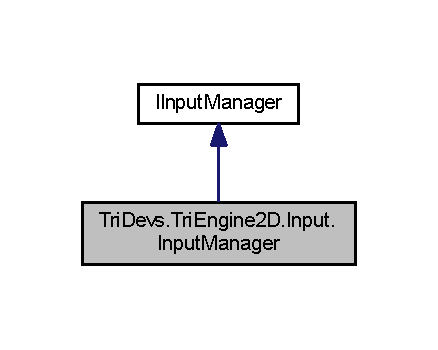
\includegraphics[width=210pt]{class_tri_devs_1_1_tri_engine2_d_1_1_input_1_1_input_manager__inherit__graph}
\end{center}
\end{figure}


Collaboration diagram for Tri\-Devs.\-Tri\-Engine2\-D.\-Input.\-Input\-Manager\-:\nopagebreak
\begin{figure}[H]
\begin{center}
\leavevmode
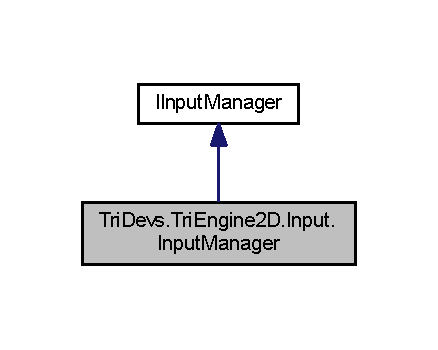
\includegraphics[width=210pt]{class_tri_devs_1_1_tri_engine2_d_1_1_input_1_1_input_manager__coll__graph}
\end{center}
\end{figure}
\subsection*{Public Member Functions}
\begin{DoxyCompactItemize}
\item 
\hyperlink{class_tri_devs_1_1_tri_engine2_d_1_1_input_1_1_input_manager_a571560933e4735d1393f697d19048b50}{Input\-Manager} ()
\begin{DoxyCompactList}\small\item\em Creates a new \hyperlink{class_tri_devs_1_1_tri_engine2_d_1_1_input_1_1_input_manager}{Input\-Manager} with only basic low-\/level input support. \end{DoxyCompactList}\item 
\hyperlink{class_tri_devs_1_1_tri_engine2_d_1_1_input_1_1_input_manager_a02702caed51c03cab2ec810cfa4b3301}{Input\-Manager} (Game\-Window window)
\begin{DoxyCompactList}\small\item\em Creates a new \hyperlink{class_tri_devs_1_1_tri_engine2_d_1_1_input_1_1_input_manager}{Input\-Manager} associated with the specified Game\-Window. \end{DoxyCompactList}\item 
void \hyperlink{class_tri_devs_1_1_tri_engine2_d_1_1_input_1_1_input_manager_a5ef0bd64a85fdafc34324cf231038302}{Update} ()
\begin{DoxyCompactList}\small\item\em Updates the input manager, refreshing all current and previous states. \end{DoxyCompactList}\item 
bool \hyperlink{class_tri_devs_1_1_tri_engine2_d_1_1_input_1_1_input_manager_a158e8ca55c8c2f972c791204cbac1b06}{Is\-Key\-Up} (Key key)
\begin{DoxyCompactList}\small\item\em Returns whether or not the specified key is currently unpressed. \end{DoxyCompactList}\item 
bool \hyperlink{class_tri_devs_1_1_tri_engine2_d_1_1_input_1_1_input_manager_a22a6938da450c2606ea779e980a33dbb}{Is\-Key\-Down} (Key key)
\begin{DoxyCompactList}\small\item\em Returns whether or not the specified key is currently being pressed. \end{DoxyCompactList}\item 
bool \hyperlink{class_tri_devs_1_1_tri_engine2_d_1_1_input_1_1_input_manager_ab3a260ea268b4683596ff5a244fd2d95}{Key\-Pressed} (Key key)
\begin{DoxyCompactList}\small\item\em Returns whether or not the specified key has been pressed. \end{DoxyCompactList}\item 
bool \hyperlink{class_tri_devs_1_1_tri_engine2_d_1_1_input_1_1_input_manager_a1e74615e2ccde33e98d262d3c48d729a}{Key\-Released} (Key key)
\begin{DoxyCompactList}\small\item\em Returns whether or not the specified key has been released. \end{DoxyCompactList}\item 
bool \hyperlink{class_tri_devs_1_1_tri_engine2_d_1_1_input_1_1_input_manager_a2d554c09767cc9f36b21f5bcde4cefa3}{Is\-Mouse\-Up} (Mouse\-Button button)
\begin{DoxyCompactList}\small\item\em Returns whether or not the specified mouse button is currently unpressed. \end{DoxyCompactList}\item 
bool \hyperlink{class_tri_devs_1_1_tri_engine2_d_1_1_input_1_1_input_manager_a6a26c5121fad6a3eefcf552a980c6ff3}{Is\-Mouse\-Down} (Mouse\-Button button)
\begin{DoxyCompactList}\small\item\em Returns whether or not the specified mouse button is currently being pressed. \end{DoxyCompactList}\item 
bool \hyperlink{class_tri_devs_1_1_tri_engine2_d_1_1_input_1_1_input_manager_a114492d5a852be9f58b3971511af3c09}{Mouse\-Pressed} (Mouse\-Button button)
\begin{DoxyCompactList}\small\item\em Returns whether or not the specified mouse button has been pressed. \end{DoxyCompactList}\item 
bool \hyperlink{class_tri_devs_1_1_tri_engine2_d_1_1_input_1_1_input_manager_aee465cfdff75ddcf53cd62aa38c09013}{Mouse\-Released} (Mouse\-Button button)
\begin{DoxyCompactList}\small\item\em Returns whether or not the specified mouse button has been released. \end{DoxyCompactList}\item 
bool \hyperlink{class_tri_devs_1_1_tri_engine2_d_1_1_input_1_1_input_manager_aa4d5c302876f5e4f99bbca7381f3d58b}{Is\-Wheel\-Up} ()
\begin{DoxyCompactList}\small\item\em Returns whether the mouse wheel was scrolled up. \end{DoxyCompactList}\item 
bool \hyperlink{class_tri_devs_1_1_tri_engine2_d_1_1_input_1_1_input_manager_a3d5c73853f0df96af5d76584bea512b2}{Is\-Wheel\-Down} ()
\begin{DoxyCompactList}\small\item\em Returns whether the mouse wheel was scrolled down. \end{DoxyCompactList}\item 
bool \hyperlink{class_tri_devs_1_1_tri_engine2_d_1_1_input_1_1_input_manager_a246df48ba2c2d15aba537f19abb806da}{Is\-Wheel\-Changed} ()
\begin{DoxyCompactList}\small\item\em Returns whether the mouse wheel scrolled at all. \end{DoxyCompactList}\item 
int \hyperlink{class_tri_devs_1_1_tri_engine2_d_1_1_input_1_1_input_manager_af8aa353e5d9434776181a42312c1499b}{Wheel\-Change} ()
\begin{DoxyCompactList}\small\item\em Returns the mouse wheel's change in value. \end{DoxyCompactList}\end{DoxyCompactItemize}
\subsection*{Properties}
\begin{DoxyCompactItemize}
\item 
int \hyperlink{class_tri_devs_1_1_tri_engine2_d_1_1_input_1_1_input_manager_afc5226998ffe43a5ee2cdd74de44d1c0}{Mouse\-X}\hspace{0.3cm}{\ttfamily  \mbox{[}get\mbox{]}}
\item 
int \hyperlink{class_tri_devs_1_1_tri_engine2_d_1_1_input_1_1_input_manager_a532a033f6ff070bc71d9fbdccda12110}{Mouse\-Y}\hspace{0.3cm}{\ttfamily  \mbox{[}get\mbox{]}}
\item 
Point$<$ int $>$ \hyperlink{class_tri_devs_1_1_tri_engine2_d_1_1_input_1_1_input_manager_aabc8216b29a248f6f352b1c979aa37b7}{Mouse\-Position}\hspace{0.3cm}{\ttfamily  \mbox{[}get\mbox{]}}
\item 
int \hyperlink{class_tri_devs_1_1_tri_engine2_d_1_1_input_1_1_input_manager_a398bf5b07143fadc5eb3e5b273f14a23}{Mouse\-Wheel\-Value}\hspace{0.3cm}{\ttfamily  \mbox{[}get\mbox{]}}
\item 
bool \hyperlink{class_tri_devs_1_1_tri_engine2_d_1_1_input_1_1_input_manager_a55645bfeff59626e79d2cfa4eee856be}{this\mbox{[}\-Key key\mbox{]}}\hspace{0.3cm}{\ttfamily  \mbox{[}get\mbox{]}}
\item 
bool \hyperlink{class_tri_devs_1_1_tri_engine2_d_1_1_input_1_1_input_manager_abe6100586cfcbfecf8197274dddf6d91}{this\mbox{[}\-Mouse\-Button button\mbox{]}}\hspace{0.3cm}{\ttfamily  \mbox{[}get\mbox{]}}
\end{DoxyCompactItemize}
\subsection*{Events}
\begin{DoxyCompactItemize}
\item 
Key\-Down\-Event\-Handler \hyperlink{class_tri_devs_1_1_tri_engine2_d_1_1_input_1_1_input_manager_af1ec1eb4d93418054f37bd17e6d6c476}{Key\-Down}
\begin{DoxyCompactList}\small\item\em Raised when a key is pressed down. \end{DoxyCompactList}\item 
Key\-Up\-Event\-Handler \hyperlink{class_tri_devs_1_1_tri_engine2_d_1_1_input_1_1_input_manager_a3435330d7f0dab7c9183122800c5a54e}{Key\-Up}
\begin{DoxyCompactList}\small\item\em Raised when a key is released. \end{DoxyCompactList}\item 
Key\-Press\-Event\-Handler \hyperlink{class_tri_devs_1_1_tri_engine2_d_1_1_input_1_1_input_manager_ad246a86523ddd915bce9c113b363d915}{Key\-Press}
\begin{DoxyCompactList}\small\item\em Raised when a character is typed. \end{DoxyCompactList}\item 
Mouse\-Down\-Event\-Handler \hyperlink{class_tri_devs_1_1_tri_engine2_d_1_1_input_1_1_input_manager_ace382adcf111fddbf706f3b5cb6be1e5}{Mouse\-Down}
\begin{DoxyCompactList}\small\item\em Raised when a mouse button is pressed down. \end{DoxyCompactList}\item 
Mouse\-Up\-Event\-Handler \hyperlink{class_tri_devs_1_1_tri_engine2_d_1_1_input_1_1_input_manager_a6597ceeecf3e9426f52c3887eb91070d}{Mouse\-Up}
\begin{DoxyCompactList}\small\item\em Raised when a mouse button is released. \end{DoxyCompactList}\item 
Mouse\-Wheel\-Changed\-Event\-Handler \hyperlink{class_tri_devs_1_1_tri_engine2_d_1_1_input_1_1_input_manager_aee07353ac8a4e9c678ff48b571e09214}{Wheel\-Changed}
\begin{DoxyCompactList}\small\item\em Raised when the mouse wheel value changes. \end{DoxyCompactList}\item 
Mouse\-Wheel\-Down\-Event\-Handler \hyperlink{class_tri_devs_1_1_tri_engine2_d_1_1_input_1_1_input_manager_a5d38d3fb1e2c2af1d89242d3708aa7af}{Wheel\-Down}
\begin{DoxyCompactList}\small\item\em Raised when the mouse wheel is scrolled downwards. \end{DoxyCompactList}\item 
Mouse\-Wheel\-Up\-Event\-Handler \hyperlink{class_tri_devs_1_1_tri_engine2_d_1_1_input_1_1_input_manager_a65ae1b2c58621de2cbc937b2e4042292}{Wheel\-Up}
\begin{DoxyCompactList}\small\item\em Raised when the mouse wheel is scrolled upwards. \end{DoxyCompactList}\end{DoxyCompactItemize}


\subsection{Detailed Description}
\hyperlink{namespace_tri_devs_1_1_tri_engine2_d_1_1_input}{Input} manager interfacing with input methods provided by a Game\-Window. 



\subsection{Constructor \& Destructor Documentation}
\hypertarget{class_tri_devs_1_1_tri_engine2_d_1_1_input_1_1_input_manager_a571560933e4735d1393f697d19048b50}{\index{Tri\-Devs\-::\-Tri\-Engine2\-D\-::\-Input\-::\-Input\-Manager@{Tri\-Devs\-::\-Tri\-Engine2\-D\-::\-Input\-::\-Input\-Manager}!Input\-Manager@{Input\-Manager}}
\index{Input\-Manager@{Input\-Manager}!TriDevs::TriEngine2D::Input::InputManager@{Tri\-Devs\-::\-Tri\-Engine2\-D\-::\-Input\-::\-Input\-Manager}}
\subsubsection[{Input\-Manager}]{\setlength{\rightskip}{0pt plus 5cm}Tri\-Devs.\-Tri\-Engine2\-D.\-Input.\-Input\-Manager.\-Input\-Manager (
\begin{DoxyParamCaption}
{}
\end{DoxyParamCaption}
)}}\label{class_tri_devs_1_1_tri_engine2_d_1_1_input_1_1_input_manager_a571560933e4735d1393f697d19048b50}


Creates a new \hyperlink{class_tri_devs_1_1_tri_engine2_d_1_1_input_1_1_input_manager}{Input\-Manager} with only basic low-\/level input support. 

Creating \hyperlink{class_tri_devs_1_1_tri_engine2_d_1_1_input_1_1_input_manager}{Input\-Manager} without a driver container will cause the events to be useless and never be raised, only the methods on this class will return any useful info. If you want event support, construct the \hyperlink{class_tri_devs_1_1_tri_engine2_d_1_1_input_1_1_input_manager}{Input\-Manager} with a Game\-Window or other supported driver providers (N\-Y\-I). 
\begin{DoxyCode}
109         \{
110             \textcolor{comment}{// We're assigning an empty mouse device.}
111             \textcolor{comment}{// This will make position functions return a constant 0.}
112             \textcolor{comment}{// Instead of being null and causing exceptions.}
113             \_mouse = \textcolor{keyword}{new} MouseDevice();
114             \textcolor{comment}{// We don't have to assign an empty keyboard device,}
115             \textcolor{comment}{// since we don't have any code that directly relies on it being present.}
116         \}
\end{DoxyCode}
\hypertarget{class_tri_devs_1_1_tri_engine2_d_1_1_input_1_1_input_manager_a02702caed51c03cab2ec810cfa4b3301}{\index{Tri\-Devs\-::\-Tri\-Engine2\-D\-::\-Input\-::\-Input\-Manager@{Tri\-Devs\-::\-Tri\-Engine2\-D\-::\-Input\-::\-Input\-Manager}!Input\-Manager@{Input\-Manager}}
\index{Input\-Manager@{Input\-Manager}!TriDevs::TriEngine2D::Input::InputManager@{Tri\-Devs\-::\-Tri\-Engine2\-D\-::\-Input\-::\-Input\-Manager}}
\subsubsection[{Input\-Manager}]{\setlength{\rightskip}{0pt plus 5cm}Tri\-Devs.\-Tri\-Engine2\-D.\-Input.\-Input\-Manager.\-Input\-Manager (
\begin{DoxyParamCaption}
\item[{Game\-Window}]{window}
\end{DoxyParamCaption}
)}}\label{class_tri_devs_1_1_tri_engine2_d_1_1_input_1_1_input_manager_a02702caed51c03cab2ec810cfa4b3301}


Creates a new \hyperlink{class_tri_devs_1_1_tri_engine2_d_1_1_input_1_1_input_manager}{Input\-Manager} associated with the specified Game\-Window. 


\begin{DoxyParams}{Parameters}
{\em window} & The Game\-Window this \hyperlink{class_tri_devs_1_1_tri_engine2_d_1_1_input_1_1_input_manager}{Input\-Manager} will interface with.\\
\hline
\end{DoxyParams}

\begin{DoxyCode}
123         \{
124             \_keyboard = window.Keyboard;
125             \_mouse = window.Mouse;
126             \_keyboard.KeyDown += OnKeyDown;
127             \_keyboard.KeyUp += OnKeyUp;
128             window.KeyPress += OnKeyPress;
129             \_mouse.ButtonDown += OnMouseDown;
130             \_mouse.ButtonUp += OnMouseUp;
131             \_mouse.WheelChanged += OnMouseWheelChanged;
132         \}
\end{DoxyCode}


\subsection{Member Function Documentation}
\hypertarget{class_tri_devs_1_1_tri_engine2_d_1_1_input_1_1_input_manager_a22a6938da450c2606ea779e980a33dbb}{\index{Tri\-Devs\-::\-Tri\-Engine2\-D\-::\-Input\-::\-Input\-Manager@{Tri\-Devs\-::\-Tri\-Engine2\-D\-::\-Input\-::\-Input\-Manager}!Is\-Key\-Down@{Is\-Key\-Down}}
\index{Is\-Key\-Down@{Is\-Key\-Down}!TriDevs::TriEngine2D::Input::InputManager@{Tri\-Devs\-::\-Tri\-Engine2\-D\-::\-Input\-::\-Input\-Manager}}
\subsubsection[{Is\-Key\-Down}]{\setlength{\rightskip}{0pt plus 5cm}bool Tri\-Devs.\-Tri\-Engine2\-D.\-Input.\-Input\-Manager.\-Is\-Key\-Down (
\begin{DoxyParamCaption}
\item[{Key}]{key}
\end{DoxyParamCaption}
)}}\label{class_tri_devs_1_1_tri_engine2_d_1_1_input_1_1_input_manager_a22a6938da450c2606ea779e980a33dbb}


Returns whether or not the specified key is currently being pressed. 


\begin{DoxyParams}{Parameters}
{\em key} & Key to query for.\\
\hline
\end{DoxyParams}
\begin{DoxyReturn}{Returns}
True if key is currently being pressed, false otherwise.
\end{DoxyReturn}


Implements \hyperlink{interface_tri_devs_1_1_tri_engine2_d_1_1_input_1_1_i_input_manager_a9f7767fe300acc7861be1e0c94ba415b}{Tri\-Devs.\-Tri\-Engine2\-D.\-Input.\-I\-Input\-Manager}.


\begin{DoxyCode}
201         \{
202             \textcolor{keywordflow}{return} \_keyboardState[key];
203         \}
\end{DoxyCode}
\hypertarget{class_tri_devs_1_1_tri_engine2_d_1_1_input_1_1_input_manager_a158e8ca55c8c2f972c791204cbac1b06}{\index{Tri\-Devs\-::\-Tri\-Engine2\-D\-::\-Input\-::\-Input\-Manager@{Tri\-Devs\-::\-Tri\-Engine2\-D\-::\-Input\-::\-Input\-Manager}!Is\-Key\-Up@{Is\-Key\-Up}}
\index{Is\-Key\-Up@{Is\-Key\-Up}!TriDevs::TriEngine2D::Input::InputManager@{Tri\-Devs\-::\-Tri\-Engine2\-D\-::\-Input\-::\-Input\-Manager}}
\subsubsection[{Is\-Key\-Up}]{\setlength{\rightskip}{0pt plus 5cm}bool Tri\-Devs.\-Tri\-Engine2\-D.\-Input.\-Input\-Manager.\-Is\-Key\-Up (
\begin{DoxyParamCaption}
\item[{Key}]{key}
\end{DoxyParamCaption}
)}}\label{class_tri_devs_1_1_tri_engine2_d_1_1_input_1_1_input_manager_a158e8ca55c8c2f972c791204cbac1b06}


Returns whether or not the specified key is currently unpressed. 


\begin{DoxyParams}{Parameters}
{\em key} & Key to query for.\\
\hline
\end{DoxyParams}
\begin{DoxyReturn}{Returns}
True if the key is currently up (not pressed), false otherwise.
\end{DoxyReturn}


Implements \hyperlink{interface_tri_devs_1_1_tri_engine2_d_1_1_input_1_1_i_input_manager_a38249eb3d1b1df7bb13835863829e8ab}{Tri\-Devs.\-Tri\-Engine2\-D.\-Input.\-I\-Input\-Manager}.


\begin{DoxyCode}
196         \{
197             \textcolor{keywordflow}{return} !\_keyboardState[key];
198         \}
\end{DoxyCode}
\hypertarget{class_tri_devs_1_1_tri_engine2_d_1_1_input_1_1_input_manager_a6a26c5121fad6a3eefcf552a980c6ff3}{\index{Tri\-Devs\-::\-Tri\-Engine2\-D\-::\-Input\-::\-Input\-Manager@{Tri\-Devs\-::\-Tri\-Engine2\-D\-::\-Input\-::\-Input\-Manager}!Is\-Mouse\-Down@{Is\-Mouse\-Down}}
\index{Is\-Mouse\-Down@{Is\-Mouse\-Down}!TriDevs::TriEngine2D::Input::InputManager@{Tri\-Devs\-::\-Tri\-Engine2\-D\-::\-Input\-::\-Input\-Manager}}
\subsubsection[{Is\-Mouse\-Down}]{\setlength{\rightskip}{0pt plus 5cm}bool Tri\-Devs.\-Tri\-Engine2\-D.\-Input.\-Input\-Manager.\-Is\-Mouse\-Down (
\begin{DoxyParamCaption}
\item[{Mouse\-Button}]{button}
\end{DoxyParamCaption}
)}}\label{class_tri_devs_1_1_tri_engine2_d_1_1_input_1_1_input_manager_a6a26c5121fad6a3eefcf552a980c6ff3}


Returns whether or not the specified mouse button is currently being pressed. 


\begin{DoxyParams}{Parameters}
{\em button} & The button to query for.\\
\hline
\end{DoxyParams}
\begin{DoxyReturn}{Returns}
True if button is currently being pressed, false otherwise.
\end{DoxyReturn}


Implements \hyperlink{interface_tri_devs_1_1_tri_engine2_d_1_1_input_1_1_i_input_manager_aa6a017570fcda20760b7e491b8351574}{Tri\-Devs.\-Tri\-Engine2\-D.\-Input.\-I\-Input\-Manager}.


\begin{DoxyCode}
221         \{
222             \textcolor{keywordflow}{return} \_mouseState[button];
223         \}
\end{DoxyCode}
\hypertarget{class_tri_devs_1_1_tri_engine2_d_1_1_input_1_1_input_manager_a2d554c09767cc9f36b21f5bcde4cefa3}{\index{Tri\-Devs\-::\-Tri\-Engine2\-D\-::\-Input\-::\-Input\-Manager@{Tri\-Devs\-::\-Tri\-Engine2\-D\-::\-Input\-::\-Input\-Manager}!Is\-Mouse\-Up@{Is\-Mouse\-Up}}
\index{Is\-Mouse\-Up@{Is\-Mouse\-Up}!TriDevs::TriEngine2D::Input::InputManager@{Tri\-Devs\-::\-Tri\-Engine2\-D\-::\-Input\-::\-Input\-Manager}}
\subsubsection[{Is\-Mouse\-Up}]{\setlength{\rightskip}{0pt plus 5cm}bool Tri\-Devs.\-Tri\-Engine2\-D.\-Input.\-Input\-Manager.\-Is\-Mouse\-Up (
\begin{DoxyParamCaption}
\item[{Mouse\-Button}]{button}
\end{DoxyParamCaption}
)}}\label{class_tri_devs_1_1_tri_engine2_d_1_1_input_1_1_input_manager_a2d554c09767cc9f36b21f5bcde4cefa3}


Returns whether or not the specified mouse button is currently unpressed. 


\begin{DoxyParams}{Parameters}
{\em button} & Button to query for.\\
\hline
\end{DoxyParams}
\begin{DoxyReturn}{Returns}
True if the button is currently up (not pressed), false otherwise.
\end{DoxyReturn}


Implements \hyperlink{interface_tri_devs_1_1_tri_engine2_d_1_1_input_1_1_i_input_manager_a40407fe8d40fe3016c9d086dd4917be4}{Tri\-Devs.\-Tri\-Engine2\-D.\-Input.\-I\-Input\-Manager}.


\begin{DoxyCode}
216         \{
217             \textcolor{keywordflow}{return} !\_mouseState[button];
218         \}
\end{DoxyCode}
\hypertarget{class_tri_devs_1_1_tri_engine2_d_1_1_input_1_1_input_manager_a246df48ba2c2d15aba537f19abb806da}{\index{Tri\-Devs\-::\-Tri\-Engine2\-D\-::\-Input\-::\-Input\-Manager@{Tri\-Devs\-::\-Tri\-Engine2\-D\-::\-Input\-::\-Input\-Manager}!Is\-Wheel\-Changed@{Is\-Wheel\-Changed}}
\index{Is\-Wheel\-Changed@{Is\-Wheel\-Changed}!TriDevs::TriEngine2D::Input::InputManager@{Tri\-Devs\-::\-Tri\-Engine2\-D\-::\-Input\-::\-Input\-Manager}}
\subsubsection[{Is\-Wheel\-Changed}]{\setlength{\rightskip}{0pt plus 5cm}bool Tri\-Devs.\-Tri\-Engine2\-D.\-Input.\-Input\-Manager.\-Is\-Wheel\-Changed (
\begin{DoxyParamCaption}
{}
\end{DoxyParamCaption}
)}}\label{class_tri_devs_1_1_tri_engine2_d_1_1_input_1_1_input_manager_a246df48ba2c2d15aba537f19abb806da}


Returns whether the mouse wheel scrolled at all. 

\begin{DoxyReturn}{Returns}
True if the mouse wheel scrolled, false otherwise.
\end{DoxyReturn}


Implements \hyperlink{interface_tri_devs_1_1_tri_engine2_d_1_1_input_1_1_i_input_manager_af7aeda5d94a3dc5e60384e4a62f84fd2}{Tri\-Devs.\-Tri\-Engine2\-D.\-Input.\-I\-Input\-Manager}.


\begin{DoxyCode}
246         \{
247             \textcolor{keywordflow}{return} \_mouseState.Wheel != \_lastMouseState.Wheel;
248         \}
\end{DoxyCode}
\hypertarget{class_tri_devs_1_1_tri_engine2_d_1_1_input_1_1_input_manager_a3d5c73853f0df96af5d76584bea512b2}{\index{Tri\-Devs\-::\-Tri\-Engine2\-D\-::\-Input\-::\-Input\-Manager@{Tri\-Devs\-::\-Tri\-Engine2\-D\-::\-Input\-::\-Input\-Manager}!Is\-Wheel\-Down@{Is\-Wheel\-Down}}
\index{Is\-Wheel\-Down@{Is\-Wheel\-Down}!TriDevs::TriEngine2D::Input::InputManager@{Tri\-Devs\-::\-Tri\-Engine2\-D\-::\-Input\-::\-Input\-Manager}}
\subsubsection[{Is\-Wheel\-Down}]{\setlength{\rightskip}{0pt plus 5cm}bool Tri\-Devs.\-Tri\-Engine2\-D.\-Input.\-Input\-Manager.\-Is\-Wheel\-Down (
\begin{DoxyParamCaption}
{}
\end{DoxyParamCaption}
)}}\label{class_tri_devs_1_1_tri_engine2_d_1_1_input_1_1_input_manager_a3d5c73853f0df96af5d76584bea512b2}


Returns whether the mouse wheel was scrolled down. 

\begin{DoxyReturn}{Returns}
True if mouse wheel was scrolled down, false otherwise.
\end{DoxyReturn}


Implements \hyperlink{interface_tri_devs_1_1_tri_engine2_d_1_1_input_1_1_i_input_manager_a01e7bb0f8255bb071678e7bcb86b97a3}{Tri\-Devs.\-Tri\-Engine2\-D.\-Input.\-I\-Input\-Manager}.


\begin{DoxyCode}
241         \{
242             \textcolor{keywordflow}{return} \_mouseState.Wheel < \_lastMouseState.Wheel;
243         \}
\end{DoxyCode}
\hypertarget{class_tri_devs_1_1_tri_engine2_d_1_1_input_1_1_input_manager_aa4d5c302876f5e4f99bbca7381f3d58b}{\index{Tri\-Devs\-::\-Tri\-Engine2\-D\-::\-Input\-::\-Input\-Manager@{Tri\-Devs\-::\-Tri\-Engine2\-D\-::\-Input\-::\-Input\-Manager}!Is\-Wheel\-Up@{Is\-Wheel\-Up}}
\index{Is\-Wheel\-Up@{Is\-Wheel\-Up}!TriDevs::TriEngine2D::Input::InputManager@{Tri\-Devs\-::\-Tri\-Engine2\-D\-::\-Input\-::\-Input\-Manager}}
\subsubsection[{Is\-Wheel\-Up}]{\setlength{\rightskip}{0pt plus 5cm}bool Tri\-Devs.\-Tri\-Engine2\-D.\-Input.\-Input\-Manager.\-Is\-Wheel\-Up (
\begin{DoxyParamCaption}
{}
\end{DoxyParamCaption}
)}}\label{class_tri_devs_1_1_tri_engine2_d_1_1_input_1_1_input_manager_aa4d5c302876f5e4f99bbca7381f3d58b}


Returns whether the mouse wheel was scrolled up. 

\begin{DoxyReturn}{Returns}
True if mouse wheel was scrolled up, false otherwise.
\end{DoxyReturn}


Implements \hyperlink{interface_tri_devs_1_1_tri_engine2_d_1_1_input_1_1_i_input_manager_a0d298286b93f065e054a2d3e9fdc4073}{Tri\-Devs.\-Tri\-Engine2\-D.\-Input.\-I\-Input\-Manager}.


\begin{DoxyCode}
236         \{
237             \textcolor{keywordflow}{return} \_mouseState.Wheel > \_lastMouseState.Wheel;
238         \}
\end{DoxyCode}
\hypertarget{class_tri_devs_1_1_tri_engine2_d_1_1_input_1_1_input_manager_ab3a260ea268b4683596ff5a244fd2d95}{\index{Tri\-Devs\-::\-Tri\-Engine2\-D\-::\-Input\-::\-Input\-Manager@{Tri\-Devs\-::\-Tri\-Engine2\-D\-::\-Input\-::\-Input\-Manager}!Key\-Pressed@{Key\-Pressed}}
\index{Key\-Pressed@{Key\-Pressed}!TriDevs::TriEngine2D::Input::InputManager@{Tri\-Devs\-::\-Tri\-Engine2\-D\-::\-Input\-::\-Input\-Manager}}
\subsubsection[{Key\-Pressed}]{\setlength{\rightskip}{0pt plus 5cm}bool Tri\-Devs.\-Tri\-Engine2\-D.\-Input.\-Input\-Manager.\-Key\-Pressed (
\begin{DoxyParamCaption}
\item[{Key}]{key}
\end{DoxyParamCaption}
)}}\label{class_tri_devs_1_1_tri_engine2_d_1_1_input_1_1_input_manager_ab3a260ea268b4683596ff5a244fd2d95}


Returns whether or not the specified key has been pressed. 

Only returns true if the last state of the key was not pressed. 


\begin{DoxyParams}{Parameters}
{\em key} & Key to query for.\\
\hline
\end{DoxyParams}
\begin{DoxyReturn}{Returns}
True if key was pressed, false otherwise.
\end{DoxyReturn}


Implements \hyperlink{interface_tri_devs_1_1_tri_engine2_d_1_1_input_1_1_i_input_manager_a0dcc608b0c3ffb806262c9f829373dcb}{Tri\-Devs.\-Tri\-Engine2\-D.\-Input.\-I\-Input\-Manager}.


\begin{DoxyCode}
206         \{
207             \textcolor{keywordflow}{return} \_keyboardState[key] && !\_lastKeyboardState[key];
208         \}
\end{DoxyCode}
\hypertarget{class_tri_devs_1_1_tri_engine2_d_1_1_input_1_1_input_manager_a1e74615e2ccde33e98d262d3c48d729a}{\index{Tri\-Devs\-::\-Tri\-Engine2\-D\-::\-Input\-::\-Input\-Manager@{Tri\-Devs\-::\-Tri\-Engine2\-D\-::\-Input\-::\-Input\-Manager}!Key\-Released@{Key\-Released}}
\index{Key\-Released@{Key\-Released}!TriDevs::TriEngine2D::Input::InputManager@{Tri\-Devs\-::\-Tri\-Engine2\-D\-::\-Input\-::\-Input\-Manager}}
\subsubsection[{Key\-Released}]{\setlength{\rightskip}{0pt plus 5cm}bool Tri\-Devs.\-Tri\-Engine2\-D.\-Input.\-Input\-Manager.\-Key\-Released (
\begin{DoxyParamCaption}
\item[{Key}]{key}
\end{DoxyParamCaption}
)}}\label{class_tri_devs_1_1_tri_engine2_d_1_1_input_1_1_input_manager_a1e74615e2ccde33e98d262d3c48d729a}


Returns whether or not the specified key has been released. 

Only returns true if the last state of the key was pressed. 


\begin{DoxyParams}{Parameters}
{\em key} & Key to query for.\\
\hline
\end{DoxyParams}
\begin{DoxyReturn}{Returns}
True if key was released, false otherwise.
\end{DoxyReturn}


Implements \hyperlink{interface_tri_devs_1_1_tri_engine2_d_1_1_input_1_1_i_input_manager_a54feb5f23a217ad5bcd104cc8912247b}{Tri\-Devs.\-Tri\-Engine2\-D.\-Input.\-I\-Input\-Manager}.


\begin{DoxyCode}
211         \{
212             \textcolor{keywordflow}{return} !\_keyboardState[key] && \_lastKeyboardState[key];
213         \}
\end{DoxyCode}
\hypertarget{class_tri_devs_1_1_tri_engine2_d_1_1_input_1_1_input_manager_a114492d5a852be9f58b3971511af3c09}{\index{Tri\-Devs\-::\-Tri\-Engine2\-D\-::\-Input\-::\-Input\-Manager@{Tri\-Devs\-::\-Tri\-Engine2\-D\-::\-Input\-::\-Input\-Manager}!Mouse\-Pressed@{Mouse\-Pressed}}
\index{Mouse\-Pressed@{Mouse\-Pressed}!TriDevs::TriEngine2D::Input::InputManager@{Tri\-Devs\-::\-Tri\-Engine2\-D\-::\-Input\-::\-Input\-Manager}}
\subsubsection[{Mouse\-Pressed}]{\setlength{\rightskip}{0pt plus 5cm}bool Tri\-Devs.\-Tri\-Engine2\-D.\-Input.\-Input\-Manager.\-Mouse\-Pressed (
\begin{DoxyParamCaption}
\item[{Mouse\-Button}]{button}
\end{DoxyParamCaption}
)}}\label{class_tri_devs_1_1_tri_engine2_d_1_1_input_1_1_input_manager_a114492d5a852be9f58b3971511af3c09}


Returns whether or not the specified mouse button has been pressed. 

Only returns true if the last state of the mouse button was not pressed. 


\begin{DoxyParams}{Parameters}
{\em button} & Button to query for.\\
\hline
\end{DoxyParams}
\begin{DoxyReturn}{Returns}
True if button was pressed, false otherwise.
\end{DoxyReturn}


Implements \hyperlink{interface_tri_devs_1_1_tri_engine2_d_1_1_input_1_1_i_input_manager_a83a14eebbb3a994cdb1a2dfcf387b4cb}{Tri\-Devs.\-Tri\-Engine2\-D.\-Input.\-I\-Input\-Manager}.


\begin{DoxyCode}
226         \{
227             \textcolor{keywordflow}{return} \_mouseState[button] && !\_lastMouseState[button];
228         \}
\end{DoxyCode}
\hypertarget{class_tri_devs_1_1_tri_engine2_d_1_1_input_1_1_input_manager_aee465cfdff75ddcf53cd62aa38c09013}{\index{Tri\-Devs\-::\-Tri\-Engine2\-D\-::\-Input\-::\-Input\-Manager@{Tri\-Devs\-::\-Tri\-Engine2\-D\-::\-Input\-::\-Input\-Manager}!Mouse\-Released@{Mouse\-Released}}
\index{Mouse\-Released@{Mouse\-Released}!TriDevs::TriEngine2D::Input::InputManager@{Tri\-Devs\-::\-Tri\-Engine2\-D\-::\-Input\-::\-Input\-Manager}}
\subsubsection[{Mouse\-Released}]{\setlength{\rightskip}{0pt plus 5cm}bool Tri\-Devs.\-Tri\-Engine2\-D.\-Input.\-Input\-Manager.\-Mouse\-Released (
\begin{DoxyParamCaption}
\item[{Mouse\-Button}]{button}
\end{DoxyParamCaption}
)}}\label{class_tri_devs_1_1_tri_engine2_d_1_1_input_1_1_input_manager_aee465cfdff75ddcf53cd62aa38c09013}


Returns whether or not the specified mouse button has been released. 

Only returns true if the last state of the button was pressed. 


\begin{DoxyParams}{Parameters}
{\em button} & The button to query for.\\
\hline
\end{DoxyParams}
\begin{DoxyReturn}{Returns}
True if the button was released, false otherwise.
\end{DoxyReturn}


Implements \hyperlink{interface_tri_devs_1_1_tri_engine2_d_1_1_input_1_1_i_input_manager_ad73037492d302fb465532f4000b76478}{Tri\-Devs.\-Tri\-Engine2\-D.\-Input.\-I\-Input\-Manager}.


\begin{DoxyCode}
231         \{
232             \textcolor{keywordflow}{return} !\_mouseState[button] && \_lastMouseState[button];
233         \}
\end{DoxyCode}
\hypertarget{class_tri_devs_1_1_tri_engine2_d_1_1_input_1_1_input_manager_a5ef0bd64a85fdafc34324cf231038302}{\index{Tri\-Devs\-::\-Tri\-Engine2\-D\-::\-Input\-::\-Input\-Manager@{Tri\-Devs\-::\-Tri\-Engine2\-D\-::\-Input\-::\-Input\-Manager}!Update@{Update}}
\index{Update@{Update}!TriDevs::TriEngine2D::Input::InputManager@{Tri\-Devs\-::\-Tri\-Engine2\-D\-::\-Input\-::\-Input\-Manager}}
\subsubsection[{Update}]{\setlength{\rightskip}{0pt plus 5cm}void Tri\-Devs.\-Tri\-Engine2\-D.\-Input.\-Input\-Manager.\-Update (
\begin{DoxyParamCaption}
{}
\end{DoxyParamCaption}
)}}\label{class_tri_devs_1_1_tri_engine2_d_1_1_input_1_1_input_manager_a5ef0bd64a85fdafc34324cf231038302}


Updates the input manager, refreshing all current and previous states. 



Implements \hyperlink{interface_tri_devs_1_1_tri_engine2_d_1_1_input_1_1_i_input_manager_a0cc046decb859d0f4d0b23a5a83d078f}{Tri\-Devs.\-Tri\-Engine2\-D.\-Input.\-I\-Input\-Manager}.


\begin{DoxyCode}
187         \{
188             \_lastKeyboardState = \_keyboardState;
189             \_keyboardState = Keyboard.GetState();
190 
191             \_lastMouseState = \_mouseState;
192             \_mouseState = Mouse.GetState();
193         \}
\end{DoxyCode}
\hypertarget{class_tri_devs_1_1_tri_engine2_d_1_1_input_1_1_input_manager_af8aa353e5d9434776181a42312c1499b}{\index{Tri\-Devs\-::\-Tri\-Engine2\-D\-::\-Input\-::\-Input\-Manager@{Tri\-Devs\-::\-Tri\-Engine2\-D\-::\-Input\-::\-Input\-Manager}!Wheel\-Change@{Wheel\-Change}}
\index{Wheel\-Change@{Wheel\-Change}!TriDevs::TriEngine2D::Input::InputManager@{Tri\-Devs\-::\-Tri\-Engine2\-D\-::\-Input\-::\-Input\-Manager}}
\subsubsection[{Wheel\-Change}]{\setlength{\rightskip}{0pt plus 5cm}int Tri\-Devs.\-Tri\-Engine2\-D.\-Input.\-Input\-Manager.\-Wheel\-Change (
\begin{DoxyParamCaption}
{}
\end{DoxyParamCaption}
)}}\label{class_tri_devs_1_1_tri_engine2_d_1_1_input_1_1_input_manager_af8aa353e5d9434776181a42312c1499b}


Returns the mouse wheel's change in value. 

\begin{DoxyReturn}{Returns}
Negative value if wheel scrolled down, positive value if scrolled up, zero if not scrolled.
\end{DoxyReturn}


Implements \hyperlink{interface_tri_devs_1_1_tri_engine2_d_1_1_input_1_1_i_input_manager_afbd3f200724d419be432da3a2dc639bd}{Tri\-Devs.\-Tri\-Engine2\-D.\-Input.\-I\-Input\-Manager}.


\begin{DoxyCode}
251         \{
252             \textcolor{keywordflow}{return} \_mouseState.Wheel - \_lastMouseState.Wheel;
253         \}
\end{DoxyCode}


\subsection{Property Documentation}
\hypertarget{class_tri_devs_1_1_tri_engine2_d_1_1_input_1_1_input_manager_aabc8216b29a248f6f352b1c979aa37b7}{\index{Tri\-Devs\-::\-Tri\-Engine2\-D\-::\-Input\-::\-Input\-Manager@{Tri\-Devs\-::\-Tri\-Engine2\-D\-::\-Input\-::\-Input\-Manager}!Mouse\-Position@{Mouse\-Position}}
\index{Mouse\-Position@{Mouse\-Position}!TriDevs::TriEngine2D::Input::InputManager@{Tri\-Devs\-::\-Tri\-Engine2\-D\-::\-Input\-::\-Input\-Manager}}
\subsubsection[{Mouse\-Position}]{\setlength{\rightskip}{0pt plus 5cm}Point$<$int$>$ Tri\-Devs.\-Tri\-Engine2\-D.\-Input.\-Input\-Manager.\-Mouse\-Position\hspace{0.3cm}{\ttfamily [get]}}}\label{class_tri_devs_1_1_tri_engine2_d_1_1_input_1_1_input_manager_aabc8216b29a248f6f352b1c979aa37b7}
\hypertarget{class_tri_devs_1_1_tri_engine2_d_1_1_input_1_1_input_manager_a398bf5b07143fadc5eb3e5b273f14a23}{\index{Tri\-Devs\-::\-Tri\-Engine2\-D\-::\-Input\-::\-Input\-Manager@{Tri\-Devs\-::\-Tri\-Engine2\-D\-::\-Input\-::\-Input\-Manager}!Mouse\-Wheel\-Value@{Mouse\-Wheel\-Value}}
\index{Mouse\-Wheel\-Value@{Mouse\-Wheel\-Value}!TriDevs::TriEngine2D::Input::InputManager@{Tri\-Devs\-::\-Tri\-Engine2\-D\-::\-Input\-::\-Input\-Manager}}
\subsubsection[{Mouse\-Wheel\-Value}]{\setlength{\rightskip}{0pt plus 5cm}int Tri\-Devs.\-Tri\-Engine2\-D.\-Input.\-Input\-Manager.\-Mouse\-Wheel\-Value\hspace{0.3cm}{\ttfamily [get]}}}\label{class_tri_devs_1_1_tri_engine2_d_1_1_input_1_1_input_manager_a398bf5b07143fadc5eb3e5b273f14a23}
\hypertarget{class_tri_devs_1_1_tri_engine2_d_1_1_input_1_1_input_manager_afc5226998ffe43a5ee2cdd74de44d1c0}{\index{Tri\-Devs\-::\-Tri\-Engine2\-D\-::\-Input\-::\-Input\-Manager@{Tri\-Devs\-::\-Tri\-Engine2\-D\-::\-Input\-::\-Input\-Manager}!Mouse\-X@{Mouse\-X}}
\index{Mouse\-X@{Mouse\-X}!TriDevs::TriEngine2D::Input::InputManager@{Tri\-Devs\-::\-Tri\-Engine2\-D\-::\-Input\-::\-Input\-Manager}}
\subsubsection[{Mouse\-X}]{\setlength{\rightskip}{0pt plus 5cm}int Tri\-Devs.\-Tri\-Engine2\-D.\-Input.\-Input\-Manager.\-Mouse\-X\hspace{0.3cm}{\ttfamily [get]}}}\label{class_tri_devs_1_1_tri_engine2_d_1_1_input_1_1_input_manager_afc5226998ffe43a5ee2cdd74de44d1c0}
\hypertarget{class_tri_devs_1_1_tri_engine2_d_1_1_input_1_1_input_manager_a532a033f6ff070bc71d9fbdccda12110}{\index{Tri\-Devs\-::\-Tri\-Engine2\-D\-::\-Input\-::\-Input\-Manager@{Tri\-Devs\-::\-Tri\-Engine2\-D\-::\-Input\-::\-Input\-Manager}!Mouse\-Y@{Mouse\-Y}}
\index{Mouse\-Y@{Mouse\-Y}!TriDevs::TriEngine2D::Input::InputManager@{Tri\-Devs\-::\-Tri\-Engine2\-D\-::\-Input\-::\-Input\-Manager}}
\subsubsection[{Mouse\-Y}]{\setlength{\rightskip}{0pt plus 5cm}int Tri\-Devs.\-Tri\-Engine2\-D.\-Input.\-Input\-Manager.\-Mouse\-Y\hspace{0.3cm}{\ttfamily [get]}}}\label{class_tri_devs_1_1_tri_engine2_d_1_1_input_1_1_input_manager_a532a033f6ff070bc71d9fbdccda12110}
\hypertarget{class_tri_devs_1_1_tri_engine2_d_1_1_input_1_1_input_manager_a55645bfeff59626e79d2cfa4eee856be}{\index{Tri\-Devs\-::\-Tri\-Engine2\-D\-::\-Input\-::\-Input\-Manager@{Tri\-Devs\-::\-Tri\-Engine2\-D\-::\-Input\-::\-Input\-Manager}!this\mbox{[}\-Key key\mbox{]}@{this[Key key]}}
\index{this\mbox{[}\-Key key\mbox{]}@{this[Key key]}!TriDevs::TriEngine2D::Input::InputManager@{Tri\-Devs\-::\-Tri\-Engine2\-D\-::\-Input\-::\-Input\-Manager}}
\subsubsection[{this[Key key]}]{\setlength{\rightskip}{0pt plus 5cm}bool Tri\-Devs.\-Tri\-Engine2\-D.\-Input.\-Input\-Manager.\-this\mbox{[}Key key\mbox{]}\hspace{0.3cm}{\ttfamily [get]}}}\label{class_tri_devs_1_1_tri_engine2_d_1_1_input_1_1_input_manager_a55645bfeff59626e79d2cfa4eee856be}
\hypertarget{class_tri_devs_1_1_tri_engine2_d_1_1_input_1_1_input_manager_abe6100586cfcbfecf8197274dddf6d91}{\index{Tri\-Devs\-::\-Tri\-Engine2\-D\-::\-Input\-::\-Input\-Manager@{Tri\-Devs\-::\-Tri\-Engine2\-D\-::\-Input\-::\-Input\-Manager}!this\mbox{[}\-Mouse\-Button button\mbox{]}@{this[Mouse\-Button button]}}
\index{this\mbox{[}\-Mouse\-Button button\mbox{]}@{this[Mouse\-Button button]}!TriDevs::TriEngine2D::Input::InputManager@{Tri\-Devs\-::\-Tri\-Engine2\-D\-::\-Input\-::\-Input\-Manager}}
\subsubsection[{this[Mouse\-Button button]}]{\setlength{\rightskip}{0pt plus 5cm}bool Tri\-Devs.\-Tri\-Engine2\-D.\-Input.\-Input\-Manager.\-this\mbox{[}Mouse\-Button button\mbox{]}\hspace{0.3cm}{\ttfamily [get]}}}\label{class_tri_devs_1_1_tri_engine2_d_1_1_input_1_1_input_manager_abe6100586cfcbfecf8197274dddf6d91}


\subsection{Event Documentation}
\hypertarget{class_tri_devs_1_1_tri_engine2_d_1_1_input_1_1_input_manager_af1ec1eb4d93418054f37bd17e6d6c476}{\index{Tri\-Devs\-::\-Tri\-Engine2\-D\-::\-Input\-::\-Input\-Manager@{Tri\-Devs\-::\-Tri\-Engine2\-D\-::\-Input\-::\-Input\-Manager}!Key\-Down@{Key\-Down}}
\index{Key\-Down@{Key\-Down}!TriDevs::TriEngine2D::Input::InputManager@{Tri\-Devs\-::\-Tri\-Engine2\-D\-::\-Input\-::\-Input\-Manager}}
\subsubsection[{Key\-Down}]{\setlength{\rightskip}{0pt plus 5cm}Key\-Down\-Event\-Handler Tri\-Devs.\-Tri\-Engine2\-D.\-Input.\-Input\-Manager.\-Key\-Down}}\label{class_tri_devs_1_1_tri_engine2_d_1_1_input_1_1_input_manager_af1ec1eb4d93418054f37bd17e6d6c476}


Raised when a key is pressed down. 

\hypertarget{class_tri_devs_1_1_tri_engine2_d_1_1_input_1_1_input_manager_ad246a86523ddd915bce9c113b363d915}{\index{Tri\-Devs\-::\-Tri\-Engine2\-D\-::\-Input\-::\-Input\-Manager@{Tri\-Devs\-::\-Tri\-Engine2\-D\-::\-Input\-::\-Input\-Manager}!Key\-Press@{Key\-Press}}
\index{Key\-Press@{Key\-Press}!TriDevs::TriEngine2D::Input::InputManager@{Tri\-Devs\-::\-Tri\-Engine2\-D\-::\-Input\-::\-Input\-Manager}}
\subsubsection[{Key\-Press}]{\setlength{\rightskip}{0pt plus 5cm}Key\-Press\-Event\-Handler Tri\-Devs.\-Tri\-Engine2\-D.\-Input.\-Input\-Manager.\-Key\-Press}}\label{class_tri_devs_1_1_tri_engine2_d_1_1_input_1_1_input_manager_ad246a86523ddd915bce9c113b363d915}


Raised when a character is typed. 

\hypertarget{class_tri_devs_1_1_tri_engine2_d_1_1_input_1_1_input_manager_a3435330d7f0dab7c9183122800c5a54e}{\index{Tri\-Devs\-::\-Tri\-Engine2\-D\-::\-Input\-::\-Input\-Manager@{Tri\-Devs\-::\-Tri\-Engine2\-D\-::\-Input\-::\-Input\-Manager}!Key\-Up@{Key\-Up}}
\index{Key\-Up@{Key\-Up}!TriDevs::TriEngine2D::Input::InputManager@{Tri\-Devs\-::\-Tri\-Engine2\-D\-::\-Input\-::\-Input\-Manager}}
\subsubsection[{Key\-Up}]{\setlength{\rightskip}{0pt plus 5cm}Key\-Up\-Event\-Handler Tri\-Devs.\-Tri\-Engine2\-D.\-Input.\-Input\-Manager.\-Key\-Up}}\label{class_tri_devs_1_1_tri_engine2_d_1_1_input_1_1_input_manager_a3435330d7f0dab7c9183122800c5a54e}


Raised when a key is released. 

\hypertarget{class_tri_devs_1_1_tri_engine2_d_1_1_input_1_1_input_manager_ace382adcf111fddbf706f3b5cb6be1e5}{\index{Tri\-Devs\-::\-Tri\-Engine2\-D\-::\-Input\-::\-Input\-Manager@{Tri\-Devs\-::\-Tri\-Engine2\-D\-::\-Input\-::\-Input\-Manager}!Mouse\-Down@{Mouse\-Down}}
\index{Mouse\-Down@{Mouse\-Down}!TriDevs::TriEngine2D::Input::InputManager@{Tri\-Devs\-::\-Tri\-Engine2\-D\-::\-Input\-::\-Input\-Manager}}
\subsubsection[{Mouse\-Down}]{\setlength{\rightskip}{0pt plus 5cm}Mouse\-Down\-Event\-Handler Tri\-Devs.\-Tri\-Engine2\-D.\-Input.\-Input\-Manager.\-Mouse\-Down}}\label{class_tri_devs_1_1_tri_engine2_d_1_1_input_1_1_input_manager_ace382adcf111fddbf706f3b5cb6be1e5}


Raised when a mouse button is pressed down. 

\hypertarget{class_tri_devs_1_1_tri_engine2_d_1_1_input_1_1_input_manager_a6597ceeecf3e9426f52c3887eb91070d}{\index{Tri\-Devs\-::\-Tri\-Engine2\-D\-::\-Input\-::\-Input\-Manager@{Tri\-Devs\-::\-Tri\-Engine2\-D\-::\-Input\-::\-Input\-Manager}!Mouse\-Up@{Mouse\-Up}}
\index{Mouse\-Up@{Mouse\-Up}!TriDevs::TriEngine2D::Input::InputManager@{Tri\-Devs\-::\-Tri\-Engine2\-D\-::\-Input\-::\-Input\-Manager}}
\subsubsection[{Mouse\-Up}]{\setlength{\rightskip}{0pt plus 5cm}Mouse\-Up\-Event\-Handler Tri\-Devs.\-Tri\-Engine2\-D.\-Input.\-Input\-Manager.\-Mouse\-Up}}\label{class_tri_devs_1_1_tri_engine2_d_1_1_input_1_1_input_manager_a6597ceeecf3e9426f52c3887eb91070d}


Raised when a mouse button is released. 

\hypertarget{class_tri_devs_1_1_tri_engine2_d_1_1_input_1_1_input_manager_aee07353ac8a4e9c678ff48b571e09214}{\index{Tri\-Devs\-::\-Tri\-Engine2\-D\-::\-Input\-::\-Input\-Manager@{Tri\-Devs\-::\-Tri\-Engine2\-D\-::\-Input\-::\-Input\-Manager}!Wheel\-Changed@{Wheel\-Changed}}
\index{Wheel\-Changed@{Wheel\-Changed}!TriDevs::TriEngine2D::Input::InputManager@{Tri\-Devs\-::\-Tri\-Engine2\-D\-::\-Input\-::\-Input\-Manager}}
\subsubsection[{Wheel\-Changed}]{\setlength{\rightskip}{0pt plus 5cm}Mouse\-Wheel\-Changed\-Event\-Handler Tri\-Devs.\-Tri\-Engine2\-D.\-Input.\-Input\-Manager.\-Wheel\-Changed}}\label{class_tri_devs_1_1_tri_engine2_d_1_1_input_1_1_input_manager_aee07353ac8a4e9c678ff48b571e09214}


Raised when the mouse wheel value changes. 

\hypertarget{class_tri_devs_1_1_tri_engine2_d_1_1_input_1_1_input_manager_a5d38d3fb1e2c2af1d89242d3708aa7af}{\index{Tri\-Devs\-::\-Tri\-Engine2\-D\-::\-Input\-::\-Input\-Manager@{Tri\-Devs\-::\-Tri\-Engine2\-D\-::\-Input\-::\-Input\-Manager}!Wheel\-Down@{Wheel\-Down}}
\index{Wheel\-Down@{Wheel\-Down}!TriDevs::TriEngine2D::Input::InputManager@{Tri\-Devs\-::\-Tri\-Engine2\-D\-::\-Input\-::\-Input\-Manager}}
\subsubsection[{Wheel\-Down}]{\setlength{\rightskip}{0pt plus 5cm}Mouse\-Wheel\-Down\-Event\-Handler Tri\-Devs.\-Tri\-Engine2\-D.\-Input.\-Input\-Manager.\-Wheel\-Down}}\label{class_tri_devs_1_1_tri_engine2_d_1_1_input_1_1_input_manager_a5d38d3fb1e2c2af1d89242d3708aa7af}


Raised when the mouse wheel is scrolled downwards. 

\hypertarget{class_tri_devs_1_1_tri_engine2_d_1_1_input_1_1_input_manager_a65ae1b2c58621de2cbc937b2e4042292}{\index{Tri\-Devs\-::\-Tri\-Engine2\-D\-::\-Input\-::\-Input\-Manager@{Tri\-Devs\-::\-Tri\-Engine2\-D\-::\-Input\-::\-Input\-Manager}!Wheel\-Up@{Wheel\-Up}}
\index{Wheel\-Up@{Wheel\-Up}!TriDevs::TriEngine2D::Input::InputManager@{Tri\-Devs\-::\-Tri\-Engine2\-D\-::\-Input\-::\-Input\-Manager}}
\subsubsection[{Wheel\-Up}]{\setlength{\rightskip}{0pt plus 5cm}Mouse\-Wheel\-Up\-Event\-Handler Tri\-Devs.\-Tri\-Engine2\-D.\-Input.\-Input\-Manager.\-Wheel\-Up}}\label{class_tri_devs_1_1_tri_engine2_d_1_1_input_1_1_input_manager_a65ae1b2c58621de2cbc937b2e4042292}


Raised when the mouse wheel is scrolled upwards. 



The documentation for this class was generated from the following file\-:\begin{DoxyCompactItemize}
\item 
Tri\-Devs.\-Tri\-Engine2\-D/\-Input/\hyperlink{_input_manager_8cs}{Input\-Manager.\-cs}\end{DoxyCompactItemize}

\hypertarget{class_tri_devs_1_1_tri_engine2_d_1_1_helpers_1_1_i_o}{\section{Tri\-Devs.\-Tri\-Engine2\-D.\-Helpers.\-I\-O Class Reference}
\label{class_tri_devs_1_1_tri_engine2_d_1_1_helpers_1_1_i_o}\index{Tri\-Devs.\-Tri\-Engine2\-D.\-Helpers.\-I\-O@{Tri\-Devs.\-Tri\-Engine2\-D.\-Helpers.\-I\-O}}
}


Provides various helper functions for doing \hyperlink{class_tri_devs_1_1_tri_engine2_d_1_1_helpers_1_1_i_o}{I\-O} operations.  


\subsection*{Static Public Member Functions}
\begin{DoxyCompactItemize}
\item 
static string \hyperlink{class_tri_devs_1_1_tri_engine2_d_1_1_helpers_1_1_i_o_a70b2f97cd90222b5620b2219024fb930}{Get\-Absolute\-Path} (string path)
\begin{DoxyCompactList}\small\item\em Resolves the absolute path from a relative path. \end{DoxyCompactList}\end{DoxyCompactItemize}


\subsection{Detailed Description}
Provides various helper functions for doing \hyperlink{class_tri_devs_1_1_tri_engine2_d_1_1_helpers_1_1_i_o}{I\-O} operations. 



\subsection{Member Function Documentation}
\hypertarget{class_tri_devs_1_1_tri_engine2_d_1_1_helpers_1_1_i_o_a70b2f97cd90222b5620b2219024fb930}{\index{Tri\-Devs\-::\-Tri\-Engine2\-D\-::\-Helpers\-::\-I\-O@{Tri\-Devs\-::\-Tri\-Engine2\-D\-::\-Helpers\-::\-I\-O}!Get\-Absolute\-Path@{Get\-Absolute\-Path}}
\index{Get\-Absolute\-Path@{Get\-Absolute\-Path}!TriDevs::TriEngine2D::Helpers::IO@{Tri\-Devs\-::\-Tri\-Engine2\-D\-::\-Helpers\-::\-I\-O}}
\subsubsection[{Get\-Absolute\-Path}]{\setlength{\rightskip}{0pt plus 5cm}static string Tri\-Devs.\-Tri\-Engine2\-D.\-Helpers.\-I\-O.\-Get\-Absolute\-Path (
\begin{DoxyParamCaption}
\item[{string}]{path}
\end{DoxyParamCaption}
)\hspace{0.3cm}{\ttfamily [static]}}}\label{class_tri_devs_1_1_tri_engine2_d_1_1_helpers_1_1_i_o_a70b2f97cd90222b5620b2219024fb930}


Resolves the absolute path from a relative path. 


\begin{DoxyParams}{Parameters}
{\em path} & The relative path to resolve.\\
\hline
\end{DoxyParams}
\begin{DoxyReturn}{Returns}
The absolute path to the item.
\end{DoxyReturn}

\begin{DoxyCode}
39         \{
40             \textcolor{keywordflow}{return} Path.Combine(Directory.GetCurrentDirectory(), path);
41         \}
\end{DoxyCode}


The documentation for this class was generated from the following file\-:\begin{DoxyCompactItemize}
\item 
Tri\-Devs.\-Tri\-Engine2\-D/\-Helpers/\hyperlink{_i_o_8cs}{I\-O.\-cs}\end{DoxyCompactItemize}

\hypertarget{class_tri_devs_1_1_tri_engine2_d_1_1_logging_1_1_log_manager}{\section{Tri\-Devs.\-Tri\-Engine2\-D.\-Logging.\-Log\-Manager Class Reference}
\label{class_tri_devs_1_1_tri_engine2_d_1_1_logging_1_1_log_manager}\index{Tri\-Devs.\-Tri\-Engine2\-D.\-Logging.\-Log\-Manager@{Tri\-Devs.\-Tri\-Engine2\-D.\-Logging.\-Log\-Manager}}
}


Class to manage logging. I\-Log interfaces should be obtained from this class' methods, as opposed to calling default log4net methods.  


\subsection*{Static Public Member Functions}
\begin{DoxyCompactItemize}
\item 
static void \hyperlink{class_tri_devs_1_1_tri_engine2_d_1_1_logging_1_1_log_manager_ac3fa271dd594c78c0ace7bd28f0b3309}{Load\-Config} (string file=null)
\begin{DoxyCompactList}\small\item\em Load a config to use with log4net. \end{DoxyCompactList}\item 
static I\-Log \hyperlink{class_tri_devs_1_1_tri_engine2_d_1_1_logging_1_1_log_manager_a08a92793a69df04598de7e2ef26525b9}{Get\-Logger} (object sender)
\begin{DoxyCompactList}\small\item\em Gets an I\-Log object for the specified object. \end{DoxyCompactList}\item 
static void \hyperlink{class_tri_devs_1_1_tri_engine2_d_1_1_logging_1_1_log_manager_a674a0fcc99cd6101fbe655e626d3f24b}{Setup\-Console} ()
\begin{DoxyCompactList}\small\item\em Set up a new console for this process. Will not set up a console if a debugger is attached. This method does nothing if D\-E\-B\-U\-G is not \#defined. \end{DoxyCompactList}\item 
static void \hyperlink{class_tri_devs_1_1_tri_engine2_d_1_1_logging_1_1_log_manager_aa08e7d3ce6fce68baddeef73861bce50}{Destroy\-Console} ()
\begin{DoxyCompactList}\small\item\em Destroys the console associated with the process, if loaded. This method does nothing if D\-E\-B\-U\-G is not \#defined. \end{DoxyCompactList}\item 
static void \hyperlink{class_tri_devs_1_1_tri_engine2_d_1_1_logging_1_1_log_manager_a869d712123422786e4e6f738bb68bee1}{Clear\-Old\-Logs} (int days\-Old=7, string logs\-Dir=\char`\"{}logs\char`\"{})
\begin{DoxyCompactList}\small\item\em Clear logs that are older than the specified amount of days. \end{DoxyCompactList}\end{DoxyCompactItemize}


\subsection{Detailed Description}
Class to manage logging. I\-Log interfaces should be obtained from this class' methods, as opposed to calling default log4net methods. 



\subsection{Member Function Documentation}
\hypertarget{class_tri_devs_1_1_tri_engine2_d_1_1_logging_1_1_log_manager_a869d712123422786e4e6f738bb68bee1}{\index{Tri\-Devs\-::\-Tri\-Engine2\-D\-::\-Logging\-::\-Log\-Manager@{Tri\-Devs\-::\-Tri\-Engine2\-D\-::\-Logging\-::\-Log\-Manager}!Clear\-Old\-Logs@{Clear\-Old\-Logs}}
\index{Clear\-Old\-Logs@{Clear\-Old\-Logs}!TriDevs::TriEngine2D::Logging::LogManager@{Tri\-Devs\-::\-Tri\-Engine2\-D\-::\-Logging\-::\-Log\-Manager}}
\subsubsection[{Clear\-Old\-Logs}]{\setlength{\rightskip}{0pt plus 5cm}static void Tri\-Devs.\-Tri\-Engine2\-D.\-Logging.\-Log\-Manager.\-Clear\-Old\-Logs (
\begin{DoxyParamCaption}
\item[{int}]{days\-Old = {\ttfamily 7}, }
\item[{string}]{logs\-Dir = {\ttfamily \char`\"{}logs\char`\"{}}}
\end{DoxyParamCaption}
)\hspace{0.3cm}{\ttfamily [static]}}}\label{class_tri_devs_1_1_tri_engine2_d_1_1_logging_1_1_log_manager_a869d712123422786e4e6f738bb68bee1}


Clear logs that are older than the specified amount of days. 


\begin{DoxyParams}{Parameters}
{\em days\-Old} & Logs older than this amount of days will be deleted.\\
\hline
{\em logs\-Dir} & The directory to clear.\\
\hline
\end{DoxyParams}

\begin{DoxyCode}
136         \{
137             var log = \hyperlink{class_tri_devs_1_1_tri_engine2_d_1_1_logging_1_1_log_manager_a08a92793a69df04598de7e2ef26525b9}{GetLogger}(typeof(LogManager));
138 
139             log.InfoFormat(\textcolor{stringliteral}{">> ClearOldLogs(\{0\}, \(\backslash\)"\{1\}\(\backslash\)")"}, daysOld, logsDir);
140 
141             \textcolor{keywordflow}{if} (!Directory.Exists(logsDir))
142             \{
143                 log.InfoFormat(\textcolor{stringliteral}{"Directory \{0\} not found, no logs to clear"}, logsDir);
144                 log.Info(\textcolor{stringliteral}{"<< ClearOldLogs()"});
145                 \textcolor{keywordflow}{return};
146             \}
147 
148             var now = DateTime.Now;
149             var max = \textcolor{keyword}{new} TimeSpan(daysOld, 0, 0, 0);
150             var count = 0;
151             \textcolor{keywordflow}{foreach} (var file \textcolor{keywordflow}{in} from file \textcolor{keywordflow}{in} Directory.GetFiles(logsDir)
152                                  let modTime = File.GetLastAccessTime(file)
153                                  let age = now.Subtract(modTime)
154                                  where age > max
155                                  select file)
156             \{
157                 \textcolor{keywordflow}{try}
158                 \{
159                     File.Delete(file);
160                     log.InfoFormat(\textcolor{stringliteral}{"Deleted old log file: \{0\}"}, file);
161                     count++;
162                 \}
163                 \textcolor{keywordflow}{catch} (IOException ex)
164                 \{
165                     log.WarnFormat(\textcolor{stringliteral}{"Failed to delete log file: \{0\} (\{1\})"}, file, ex.Message);
166                 \}
167             \}
168 
169             log.InfoFormat(\textcolor{stringliteral}{"Done! Cleared \{0\} log files."}, count);
170             log.Info(\textcolor{stringliteral}{"<< ClearOldLogs()"});
171         \}
\end{DoxyCode}
\hypertarget{class_tri_devs_1_1_tri_engine2_d_1_1_logging_1_1_log_manager_aa08e7d3ce6fce68baddeef73861bce50}{\index{Tri\-Devs\-::\-Tri\-Engine2\-D\-::\-Logging\-::\-Log\-Manager@{Tri\-Devs\-::\-Tri\-Engine2\-D\-::\-Logging\-::\-Log\-Manager}!Destroy\-Console@{Destroy\-Console}}
\index{Destroy\-Console@{Destroy\-Console}!TriDevs::TriEngine2D::Logging::LogManager@{Tri\-Devs\-::\-Tri\-Engine2\-D\-::\-Logging\-::\-Log\-Manager}}
\subsubsection[{Destroy\-Console}]{\setlength{\rightskip}{0pt plus 5cm}static void Tri\-Devs.\-Tri\-Engine2\-D.\-Logging.\-Log\-Manager.\-Destroy\-Console (
\begin{DoxyParamCaption}
{}
\end{DoxyParamCaption}
)\hspace{0.3cm}{\ttfamily [static]}}}\label{class_tri_devs_1_1_tri_engine2_d_1_1_logging_1_1_log_manager_aa08e7d3ce6fce68baddeef73861bce50}


Destroys the console associated with the process, if loaded. This method does nothing if D\-E\-B\-U\-G is not \#defined. 


\begin{DoxyCode}
123         \{
124 \textcolor{preprocessor}{#if DEBUG}
125 \textcolor{preprocessor}{}            \textcolor{keywordflow}{if} (\_consoleLoaded)
126                 \hyperlink{class_tri_devs_1_1_tri_engine2_d_1_1_native_1_1_win_a_p_i}{WinAPI}.\hyperlink{class_tri_devs_1_1_tri_engine2_d_1_1_native_1_1_win_a_p_i_a14d148cdaa742fd0d25fd962f6c1f8c4}{FreeConsole}();
127 \textcolor{preprocessor}{#endif}
128 \textcolor{preprocessor}{}        \}
\end{DoxyCode}


Here is the call graph for this function\-:\nopagebreak
\begin{figure}[H]
\begin{center}
\leavevmode
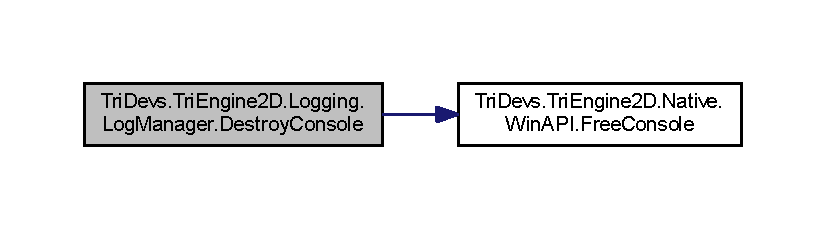
\includegraphics[width=350pt]{class_tri_devs_1_1_tri_engine2_d_1_1_logging_1_1_log_manager_aa08e7d3ce6fce68baddeef73861bce50_cgraph}
\end{center}
\end{figure}


\hypertarget{class_tri_devs_1_1_tri_engine2_d_1_1_logging_1_1_log_manager_a08a92793a69df04598de7e2ef26525b9}{\index{Tri\-Devs\-::\-Tri\-Engine2\-D\-::\-Logging\-::\-Log\-Manager@{Tri\-Devs\-::\-Tri\-Engine2\-D\-::\-Logging\-::\-Log\-Manager}!Get\-Logger@{Get\-Logger}}
\index{Get\-Logger@{Get\-Logger}!TriDevs::TriEngine2D::Logging::LogManager@{Tri\-Devs\-::\-Tri\-Engine2\-D\-::\-Logging\-::\-Log\-Manager}}
\subsubsection[{Get\-Logger}]{\setlength{\rightskip}{0pt plus 5cm}static I\-Log Tri\-Devs.\-Tri\-Engine2\-D.\-Logging.\-Log\-Manager.\-Get\-Logger (
\begin{DoxyParamCaption}
\item[{object}]{sender}
\end{DoxyParamCaption}
)\hspace{0.3cm}{\ttfamily [static]}}}\label{class_tri_devs_1_1_tri_engine2_d_1_1_logging_1_1_log_manager_a08a92793a69df04598de7e2ef26525b9}


Gets an I\-Log object for the specified object. 

To get the logger object for a static class, or from static context, call Get\-Logger(typeof(\-Your\-Class)). 


\begin{DoxyParams}{Parameters}
{\em sender} & The object or Type to get an I\-Log object for.\\
\hline
\end{DoxyParams}
\begin{DoxyReturn}{Returns}
The I\-Log object.
\end{DoxyReturn}

\begin{DoxyCode}
89         \{
90             \textcolor{keywordflow}{if} (!\_loaded)
91                 \hyperlink{class_tri_devs_1_1_tri_engine2_d_1_1_logging_1_1_log_manager_ac3fa271dd594c78c0ace7bd28f0b3309}{LoadConfig}();
92 
93             \textcolor{keywordflow}{return} log4net.LogManager.GetLogger(sender.GetType().ToString() == \textcolor{stringliteral}{"System.RuntimeType"} ? (Type
      )sender : sender.GetType());
94         \}
\end{DoxyCode}
\hypertarget{class_tri_devs_1_1_tri_engine2_d_1_1_logging_1_1_log_manager_ac3fa271dd594c78c0ace7bd28f0b3309}{\index{Tri\-Devs\-::\-Tri\-Engine2\-D\-::\-Logging\-::\-Log\-Manager@{Tri\-Devs\-::\-Tri\-Engine2\-D\-::\-Logging\-::\-Log\-Manager}!Load\-Config@{Load\-Config}}
\index{Load\-Config@{Load\-Config}!TriDevs::TriEngine2D::Logging::LogManager@{Tri\-Devs\-::\-Tri\-Engine2\-D\-::\-Logging\-::\-Log\-Manager}}
\subsubsection[{Load\-Config}]{\setlength{\rightskip}{0pt plus 5cm}static void Tri\-Devs.\-Tri\-Engine2\-D.\-Logging.\-Log\-Manager.\-Load\-Config (
\begin{DoxyParamCaption}
\item[{string}]{file = {\ttfamily null}}
\end{DoxyParamCaption}
)\hspace{0.3cm}{\ttfamily [static]}}}\label{class_tri_devs_1_1_tri_engine2_d_1_1_logging_1_1_log_manager_ac3fa271dd594c78c0ace7bd28f0b3309}


Load a config to use with log4net. 

Load\-Config will first try to load the specified file, if not null. If it is unable to find the specified file, it will call itself again with file set to null. If no file is specified, it will attempt to load a config file following the pattern\-: \char`\"{}(\-Assembly\-Name).\-config\char`\"{} If it is unable to load the config, it will default to Basic\-Configurator. 


\begin{DoxyParams}{Parameters}
{\em file} & The config file to load, null if automatic loading is preferred.\\
\hline
\end{DoxyParams}

\begin{DoxyCode}
57         \{
58             \textcolor{keywordflow}{if} (file == null)
59             \{
60                 \textcolor{keywordflow}{if} (File.Exists(AppDomain.CurrentDomain.FriendlyName + \textcolor{stringliteral}{".config"}))
61                     XmlConfigurator.Configure();
62                 \textcolor{keywordflow}{else}
63                     BasicConfigurator.Configure();
64             \}
65             \textcolor{keywordflow}{else}
66             \{
67                 \textcolor{keywordflow}{if} (File.Exists(file))
68                     XmlConfigurator.Configure(\textcolor{keyword}{new} FileInfo(file));
69                 \textcolor{keywordflow}{else}
70                 \{
71                     \hyperlink{class_tri_devs_1_1_tri_engine2_d_1_1_logging_1_1_log_manager_ac3fa271dd594c78c0ace7bd28f0b3309}{LoadConfig}();
72                     \textcolor{keywordflow}{return};
73                 \}
74             \}
75 
76             \_loaded = \textcolor{keyword}{true};
77         \}
\end{DoxyCode}
\hypertarget{class_tri_devs_1_1_tri_engine2_d_1_1_logging_1_1_log_manager_a674a0fcc99cd6101fbe655e626d3f24b}{\index{Tri\-Devs\-::\-Tri\-Engine2\-D\-::\-Logging\-::\-Log\-Manager@{Tri\-Devs\-::\-Tri\-Engine2\-D\-::\-Logging\-::\-Log\-Manager}!Setup\-Console@{Setup\-Console}}
\index{Setup\-Console@{Setup\-Console}!TriDevs::TriEngine2D::Logging::LogManager@{Tri\-Devs\-::\-Tri\-Engine2\-D\-::\-Logging\-::\-Log\-Manager}}
\subsubsection[{Setup\-Console}]{\setlength{\rightskip}{0pt plus 5cm}static void Tri\-Devs.\-Tri\-Engine2\-D.\-Logging.\-Log\-Manager.\-Setup\-Console (
\begin{DoxyParamCaption}
{}
\end{DoxyParamCaption}
)\hspace{0.3cm}{\ttfamily [static]}}}\label{class_tri_devs_1_1_tri_engine2_d_1_1_logging_1_1_log_manager_a674a0fcc99cd6101fbe655e626d3f24b}


Set up a new console for this process. Will not set up a console if a debugger is attached. This method does nothing if D\-E\-B\-U\-G is not \#defined. 


\begin{DoxyCode}
102         \{
103 \textcolor{preprocessor}{#if DEBUG}
104 \textcolor{preprocessor}{}            \textcolor{keywordflow}{if} (System.Diagnostics.Debugger.IsAttached)
105                 \textcolor{keywordflow}{return};
106 
107             \hyperlink{class_tri_devs_1_1_tri_engine2_d_1_1_native_1_1_win_a_p_i}{WinAPI}.\hyperlink{class_tri_devs_1_1_tri_engine2_d_1_1_native_1_1_win_a_p_i_a00f0889a729e989fbefd8267a20a1c06}{AllocConsole}();
108             var stdHandle = \hyperlink{class_tri_devs_1_1_tri_engine2_d_1_1_native_1_1_win_a_p_i}{WinAPI}.\hyperlink{class_tri_devs_1_1_tri_engine2_d_1_1_native_1_1_win_a_p_i_a7617bf77270291625f566cf21294d518}{GetStdHandle}(\hyperlink{class_tri_devs_1_1_tri_engine2_d_1_1_native_1_1_win_a_p_i}{WinAPI}.
      \hyperlink{class_tri_devs_1_1_tri_engine2_d_1_1_native_1_1_win_a_p_i_a19ebb40d1edf46781ea0fdf4a9c94e8b}{STD\_OUTPUT\_HANDLE});
109             var safeFileHandle = \textcolor{keyword}{new} SafeFileHandle(stdHandle, \textcolor{keyword}{true});
110             var fileStream = \textcolor{keyword}{new} FileStream(safeFileHandle, FileAccess.Write);
111             var encoding = Encoding.GetEncoding(\hyperlink{class_tri_devs_1_1_tri_engine2_d_1_1_native_1_1_win_a_p_i}{WinAPI}.\hyperlink{class_tri_devs_1_1_tri_engine2_d_1_1_native_1_1_win_a_p_i_a83ef0d2539e95cc640d8e1f1216beec5}{CODE\_PAGE});
112             var stdOut = \textcolor{keyword}{new} StreamWriter(fileStream, encoding) \{ AutoFlush = \textcolor{keyword}{true} \};
113             Console.SetOut(stdOut);
114             \_consoleLoaded = \textcolor{keyword}{true};
115 \textcolor{preprocessor}{#endif}
116 \textcolor{preprocessor}{}        \}
\end{DoxyCode}


Here is the call graph for this function\-:\nopagebreak
\begin{figure}[H]
\begin{center}
\leavevmode
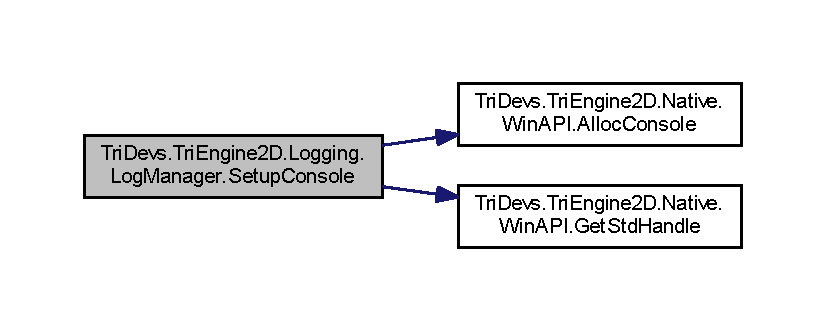
\includegraphics[width=350pt]{class_tri_devs_1_1_tri_engine2_d_1_1_logging_1_1_log_manager_a674a0fcc99cd6101fbe655e626d3f24b_cgraph}
\end{center}
\end{figure}




The documentation for this class was generated from the following file\-:\begin{DoxyCompactItemize}
\item 
Tri\-Devs.\-Tri\-Engine2\-D/\-Logging/\hyperlink{_log_manager_8cs}{Log\-Manager.\-cs}\end{DoxyCompactItemize}

\hypertarget{class_tri_devs_1_1_tri_engine2_d_1_1_input_1_1_null_input_manager}{\section{Tri\-Devs.\-Tri\-Engine2\-D.\-Input.\-Null\-Input\-Manager Class Reference}
\label{class_tri_devs_1_1_tri_engine2_d_1_1_input_1_1_null_input_manager}\index{Tri\-Devs.\-Tri\-Engine2\-D.\-Input.\-Null\-Input\-Manager@{Tri\-Devs.\-Tri\-Engine2\-D.\-Input.\-Null\-Input\-Manager}}
}


Used as a fallback \hyperlink{class_tri_devs_1_1_tri_engine2_d_1_1_input_1_1_input_manager}{Input\-Manager} object when the service locator fails to find one.  




Inheritance diagram for Tri\-Devs.\-Tri\-Engine2\-D.\-Input.\-Null\-Input\-Manager\-:\nopagebreak
\begin{figure}[H]
\begin{center}
\leavevmode
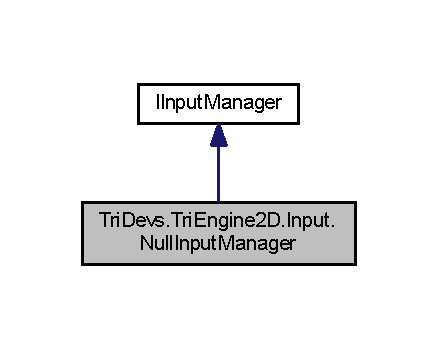
\includegraphics[width=210pt]{class_tri_devs_1_1_tri_engine2_d_1_1_input_1_1_null_input_manager__inherit__graph}
\end{center}
\end{figure}


Collaboration diagram for Tri\-Devs.\-Tri\-Engine2\-D.\-Input.\-Null\-Input\-Manager\-:\nopagebreak
\begin{figure}[H]
\begin{center}
\leavevmode
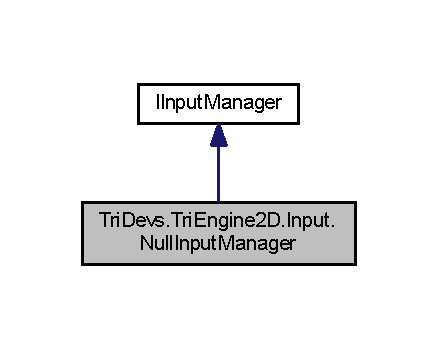
\includegraphics[width=210pt]{class_tri_devs_1_1_tri_engine2_d_1_1_input_1_1_null_input_manager__coll__graph}
\end{center}
\end{figure}
\subsection*{Public Member Functions}
\begin{DoxyCompactItemize}
\item 
void \hyperlink{class_tri_devs_1_1_tri_engine2_d_1_1_input_1_1_null_input_manager_a7713c34aa9dea7d6f0878e9c99217df3}{Update} ()
\begin{DoxyCompactList}\small\item\em Updates the input manager, refreshing all current and previous states. \end{DoxyCompactList}\item 
bool \hyperlink{class_tri_devs_1_1_tri_engine2_d_1_1_input_1_1_null_input_manager_a4d8adbdf820de7ca44cd2781c209a5ba}{Key\-Up} (Key key)
\begin{DoxyCompactList}\small\item\em Returns whether or not the specified key is currently unpressed. \end{DoxyCompactList}\item 
bool \hyperlink{class_tri_devs_1_1_tri_engine2_d_1_1_input_1_1_null_input_manager_a1079920f69a7fec078a52f99be45b24a}{Key\-Down} (Key key)
\begin{DoxyCompactList}\small\item\em Returns whether or not the specified key is currently being pressed. \end{DoxyCompactList}\item 
bool \hyperlink{class_tri_devs_1_1_tri_engine2_d_1_1_input_1_1_null_input_manager_a2de0da3893be579c99690caa0d3cd2cc}{Key\-Pressed} (Key key)
\begin{DoxyCompactList}\small\item\em Returns whether or not the specified key has been pressed. \end{DoxyCompactList}\item 
bool \hyperlink{class_tri_devs_1_1_tri_engine2_d_1_1_input_1_1_null_input_manager_aadf04bc0e73da9612c1cdd435fdb6867}{Key\-Released} (Key key)
\begin{DoxyCompactList}\small\item\em Returns whether or not the specified key has been released. \end{DoxyCompactList}\item 
bool \hyperlink{class_tri_devs_1_1_tri_engine2_d_1_1_input_1_1_null_input_manager_aa673576f2f8d44329d7876c6a450e44c}{Button\-Up} (Mouse\-Button button)
\begin{DoxyCompactList}\small\item\em Returns whether or not the specified mouse button is currently unpressed. \end{DoxyCompactList}\item 
bool \hyperlink{class_tri_devs_1_1_tri_engine2_d_1_1_input_1_1_null_input_manager_ab38069ccd3245683457aeae4acef95f8}{Button\-Down} (Mouse\-Button button)
\begin{DoxyCompactList}\small\item\em Returns whether or not the specified mouse button is currently being pressed. \end{DoxyCompactList}\item 
bool \hyperlink{class_tri_devs_1_1_tri_engine2_d_1_1_input_1_1_null_input_manager_afe0386a599a114925b1eb5476f8a64c6}{Button\-Pressed} (Mouse\-Button button)
\begin{DoxyCompactList}\small\item\em Returns whether or not the specified mouse button has been pressed. \end{DoxyCompactList}\item 
bool \hyperlink{class_tri_devs_1_1_tri_engine2_d_1_1_input_1_1_null_input_manager_a827589d1117393e7748386b6416de482}{Button\-Released} (Mouse\-Button button)
\begin{DoxyCompactList}\small\item\em Returns whether or not the specified mouse button has been released. \end{DoxyCompactList}\item 
bool \hyperlink{class_tri_devs_1_1_tri_engine2_d_1_1_input_1_1_null_input_manager_a6ffebd26487cf6673e9b71808bfd2e56}{Wheel\-Up} ()
\begin{DoxyCompactList}\small\item\em Returns whether the mouse wheel was scrolled up. \end{DoxyCompactList}\item 
bool \hyperlink{class_tri_devs_1_1_tri_engine2_d_1_1_input_1_1_null_input_manager_a438af9fe186fdb91e3fe1e9fbb00a03f}{Wheel\-Down} ()
\begin{DoxyCompactList}\small\item\em Returns whether the mouse wheel was scrolled down. \end{DoxyCompactList}\item 
bool \hyperlink{class_tri_devs_1_1_tri_engine2_d_1_1_input_1_1_null_input_manager_afc5e4eb8cd98adc0ee1aea4a4967246a}{Wheel\-Changed} ()
\begin{DoxyCompactList}\small\item\em Returns whether the mouse wheel scrolled at all. \end{DoxyCompactList}\item 
int \hyperlink{class_tri_devs_1_1_tri_engine2_d_1_1_input_1_1_null_input_manager_a48b6584ca2a845d0ae108a0e08145c43}{Wheel\-Change} ()
\begin{DoxyCompactList}\small\item\em Returns the mouse wheel's change in value. \end{DoxyCompactList}\end{DoxyCompactItemize}
\subsection*{Properties}
\begin{DoxyCompactItemize}
\item 
int \hyperlink{class_tri_devs_1_1_tri_engine2_d_1_1_input_1_1_null_input_manager_a4d2bafa6eb9ebc0be564e472c2c50cd2}{Mouse\-X}\hspace{0.3cm}{\ttfamily  \mbox{[}get\mbox{]}}
\item 
int \hyperlink{class_tri_devs_1_1_tri_engine2_d_1_1_input_1_1_null_input_manager_af5cd8b1160c3d8e89f45f2ca05d6ef5a}{Mouse\-Y}\hspace{0.3cm}{\ttfamily  \mbox{[}get\mbox{]}}
\item 
\hyperlink{struct_tri_devs_1_1_tri_engine2_d_1_1_point}{Point} \hyperlink{class_tri_devs_1_1_tri_engine2_d_1_1_input_1_1_null_input_manager_aad7209f97294a7ce7bbb9cc9295d21dd}{Mouse\-Position}\hspace{0.3cm}{\ttfamily  \mbox{[}get\mbox{]}}
\item 
int \hyperlink{class_tri_devs_1_1_tri_engine2_d_1_1_input_1_1_null_input_manager_a7afee03cecf29b1cc123fe7a03b239df}{Mouse\-Wheel\-Value}\hspace{0.3cm}{\ttfamily  \mbox{[}get\mbox{]}}
\item 
bool \hyperlink{class_tri_devs_1_1_tri_engine2_d_1_1_input_1_1_null_input_manager_ad1553333590d5c3e37df8e3ee0b6e69b}{this\mbox{[}\-Key key\mbox{]}}\hspace{0.3cm}{\ttfamily  \mbox{[}get\mbox{]}}
\item 
bool \hyperlink{class_tri_devs_1_1_tri_engine2_d_1_1_input_1_1_null_input_manager_ac72562b9f98a5865412cd12ce87c6fbb}{this\mbox{[}\-Mouse\-Button button\mbox{]}}\hspace{0.3cm}{\ttfamily  \mbox{[}get\mbox{]}}
\end{DoxyCompactItemize}


\subsection{Detailed Description}
Used as a fallback \hyperlink{class_tri_devs_1_1_tri_engine2_d_1_1_input_1_1_input_manager}{Input\-Manager} object when the service locator fails to find one. 



\subsection{Member Function Documentation}
\hypertarget{class_tri_devs_1_1_tri_engine2_d_1_1_input_1_1_null_input_manager_ab38069ccd3245683457aeae4acef95f8}{\index{Tri\-Devs\-::\-Tri\-Engine2\-D\-::\-Input\-::\-Null\-Input\-Manager@{Tri\-Devs\-::\-Tri\-Engine2\-D\-::\-Input\-::\-Null\-Input\-Manager}!Button\-Down@{Button\-Down}}
\index{Button\-Down@{Button\-Down}!TriDevs::TriEngine2D::Input::NullInputManager@{Tri\-Devs\-::\-Tri\-Engine2\-D\-::\-Input\-::\-Null\-Input\-Manager}}
\subsubsection[{Button\-Down}]{\setlength{\rightskip}{0pt plus 5cm}bool Tri\-Devs.\-Tri\-Engine2\-D.\-Input.\-Null\-Input\-Manager.\-Button\-Down (
\begin{DoxyParamCaption}
\item[{Mouse\-Button}]{button}
\end{DoxyParamCaption}
)}}\label{class_tri_devs_1_1_tri_engine2_d_1_1_input_1_1_null_input_manager_ab38069ccd3245683457aeae4acef95f8}


Returns whether or not the specified mouse button is currently being pressed. 


\begin{DoxyParams}{Parameters}
{\em button} & The button to query for.\\
\hline
\end{DoxyParams}
\begin{DoxyReturn}{Returns}
True if button is currently being pressed, false otherwise.
\end{DoxyReturn}


Implements \hyperlink{interface_tri_devs_1_1_tri_engine2_d_1_1_input_1_1_i_input_manager_a8383fd315905874db04d455211fec203}{Tri\-Devs.\-Tri\-Engine2\-D.\-Input.\-I\-Input\-Manager}.


\begin{DoxyCode}
79         \{
80             \textcolor{keywordflow}{return} \textcolor{keyword}{false};
81         \}
\end{DoxyCode}
\hypertarget{class_tri_devs_1_1_tri_engine2_d_1_1_input_1_1_null_input_manager_afe0386a599a114925b1eb5476f8a64c6}{\index{Tri\-Devs\-::\-Tri\-Engine2\-D\-::\-Input\-::\-Null\-Input\-Manager@{Tri\-Devs\-::\-Tri\-Engine2\-D\-::\-Input\-::\-Null\-Input\-Manager}!Button\-Pressed@{Button\-Pressed}}
\index{Button\-Pressed@{Button\-Pressed}!TriDevs::TriEngine2D::Input::NullInputManager@{Tri\-Devs\-::\-Tri\-Engine2\-D\-::\-Input\-::\-Null\-Input\-Manager}}
\subsubsection[{Button\-Pressed}]{\setlength{\rightskip}{0pt plus 5cm}bool Tri\-Devs.\-Tri\-Engine2\-D.\-Input.\-Null\-Input\-Manager.\-Button\-Pressed (
\begin{DoxyParamCaption}
\item[{Mouse\-Button}]{button}
\end{DoxyParamCaption}
)}}\label{class_tri_devs_1_1_tri_engine2_d_1_1_input_1_1_null_input_manager_afe0386a599a114925b1eb5476f8a64c6}


Returns whether or not the specified mouse button has been pressed. 

Only returns true if the last state of the mouse button was not pressed. 


\begin{DoxyParams}{Parameters}
{\em button} & Button to query for.\\
\hline
\end{DoxyParams}
\begin{DoxyReturn}{Returns}
True if button was pressed, false otherwise.
\end{DoxyReturn}


Implements \hyperlink{interface_tri_devs_1_1_tri_engine2_d_1_1_input_1_1_i_input_manager_a2b09825487ca4dfccbce5d91ff03bbb1}{Tri\-Devs.\-Tri\-Engine2\-D.\-Input.\-I\-Input\-Manager}.


\begin{DoxyCode}
84         \{
85             \textcolor{keywordflow}{return} \textcolor{keyword}{false};
86         \}
\end{DoxyCode}
\hypertarget{class_tri_devs_1_1_tri_engine2_d_1_1_input_1_1_null_input_manager_a827589d1117393e7748386b6416de482}{\index{Tri\-Devs\-::\-Tri\-Engine2\-D\-::\-Input\-::\-Null\-Input\-Manager@{Tri\-Devs\-::\-Tri\-Engine2\-D\-::\-Input\-::\-Null\-Input\-Manager}!Button\-Released@{Button\-Released}}
\index{Button\-Released@{Button\-Released}!TriDevs::TriEngine2D::Input::NullInputManager@{Tri\-Devs\-::\-Tri\-Engine2\-D\-::\-Input\-::\-Null\-Input\-Manager}}
\subsubsection[{Button\-Released}]{\setlength{\rightskip}{0pt plus 5cm}bool Tri\-Devs.\-Tri\-Engine2\-D.\-Input.\-Null\-Input\-Manager.\-Button\-Released (
\begin{DoxyParamCaption}
\item[{Mouse\-Button}]{button}
\end{DoxyParamCaption}
)}}\label{class_tri_devs_1_1_tri_engine2_d_1_1_input_1_1_null_input_manager_a827589d1117393e7748386b6416de482}


Returns whether or not the specified mouse button has been released. 

Only returns true if the last state of the button was pressed. 


\begin{DoxyParams}{Parameters}
{\em button} & The button to query for.\\
\hline
\end{DoxyParams}
\begin{DoxyReturn}{Returns}
True if the button was released, false otherwise.
\end{DoxyReturn}


Implements \hyperlink{interface_tri_devs_1_1_tri_engine2_d_1_1_input_1_1_i_input_manager_a42249b011c0ba487a2464d2b32e014f5}{Tri\-Devs.\-Tri\-Engine2\-D.\-Input.\-I\-Input\-Manager}.


\begin{DoxyCode}
89         \{
90             \textcolor{keywordflow}{return} \textcolor{keyword}{false};
91         \}
\end{DoxyCode}
\hypertarget{class_tri_devs_1_1_tri_engine2_d_1_1_input_1_1_null_input_manager_aa673576f2f8d44329d7876c6a450e44c}{\index{Tri\-Devs\-::\-Tri\-Engine2\-D\-::\-Input\-::\-Null\-Input\-Manager@{Tri\-Devs\-::\-Tri\-Engine2\-D\-::\-Input\-::\-Null\-Input\-Manager}!Button\-Up@{Button\-Up}}
\index{Button\-Up@{Button\-Up}!TriDevs::TriEngine2D::Input::NullInputManager@{Tri\-Devs\-::\-Tri\-Engine2\-D\-::\-Input\-::\-Null\-Input\-Manager}}
\subsubsection[{Button\-Up}]{\setlength{\rightskip}{0pt plus 5cm}bool Tri\-Devs.\-Tri\-Engine2\-D.\-Input.\-Null\-Input\-Manager.\-Button\-Up (
\begin{DoxyParamCaption}
\item[{Mouse\-Button}]{button}
\end{DoxyParamCaption}
)}}\label{class_tri_devs_1_1_tri_engine2_d_1_1_input_1_1_null_input_manager_aa673576f2f8d44329d7876c6a450e44c}


Returns whether or not the specified mouse button is currently unpressed. 


\begin{DoxyParams}{Parameters}
{\em button} & Button to query for.\\
\hline
\end{DoxyParams}
\begin{DoxyReturn}{Returns}
True if the button is currently up (not pressed), false otherwise.
\end{DoxyReturn}


Implements \hyperlink{interface_tri_devs_1_1_tri_engine2_d_1_1_input_1_1_i_input_manager_a7e3896e1a022954b73b5e6323e3c85ae}{Tri\-Devs.\-Tri\-Engine2\-D.\-Input.\-I\-Input\-Manager}.


\begin{DoxyCode}
74         \{
75             \textcolor{keywordflow}{return} \textcolor{keyword}{true};
76         \}
\end{DoxyCode}
\hypertarget{class_tri_devs_1_1_tri_engine2_d_1_1_input_1_1_null_input_manager_a1079920f69a7fec078a52f99be45b24a}{\index{Tri\-Devs\-::\-Tri\-Engine2\-D\-::\-Input\-::\-Null\-Input\-Manager@{Tri\-Devs\-::\-Tri\-Engine2\-D\-::\-Input\-::\-Null\-Input\-Manager}!Key\-Down@{Key\-Down}}
\index{Key\-Down@{Key\-Down}!TriDevs::TriEngine2D::Input::NullInputManager@{Tri\-Devs\-::\-Tri\-Engine2\-D\-::\-Input\-::\-Null\-Input\-Manager}}
\subsubsection[{Key\-Down}]{\setlength{\rightskip}{0pt plus 5cm}bool Tri\-Devs.\-Tri\-Engine2\-D.\-Input.\-Null\-Input\-Manager.\-Key\-Down (
\begin{DoxyParamCaption}
\item[{Key}]{key}
\end{DoxyParamCaption}
)}}\label{class_tri_devs_1_1_tri_engine2_d_1_1_input_1_1_null_input_manager_a1079920f69a7fec078a52f99be45b24a}


Returns whether or not the specified key is currently being pressed. 


\begin{DoxyParams}{Parameters}
{\em key} & Key to query for.\\
\hline
\end{DoxyParams}
\begin{DoxyReturn}{Returns}
True if key is currently being pressed, false otherwise.
\end{DoxyReturn}


Implements \hyperlink{interface_tri_devs_1_1_tri_engine2_d_1_1_input_1_1_i_input_manager_a380e86578e668193eb874acbd2754389}{Tri\-Devs.\-Tri\-Engine2\-D.\-Input.\-I\-Input\-Manager}.


\begin{DoxyCode}
59         \{
60             \textcolor{keywordflow}{return} \textcolor{keyword}{false};
61         \}
\end{DoxyCode}
\hypertarget{class_tri_devs_1_1_tri_engine2_d_1_1_input_1_1_null_input_manager_a2de0da3893be579c99690caa0d3cd2cc}{\index{Tri\-Devs\-::\-Tri\-Engine2\-D\-::\-Input\-::\-Null\-Input\-Manager@{Tri\-Devs\-::\-Tri\-Engine2\-D\-::\-Input\-::\-Null\-Input\-Manager}!Key\-Pressed@{Key\-Pressed}}
\index{Key\-Pressed@{Key\-Pressed}!TriDevs::TriEngine2D::Input::NullInputManager@{Tri\-Devs\-::\-Tri\-Engine2\-D\-::\-Input\-::\-Null\-Input\-Manager}}
\subsubsection[{Key\-Pressed}]{\setlength{\rightskip}{0pt plus 5cm}bool Tri\-Devs.\-Tri\-Engine2\-D.\-Input.\-Null\-Input\-Manager.\-Key\-Pressed (
\begin{DoxyParamCaption}
\item[{Key}]{key}
\end{DoxyParamCaption}
)}}\label{class_tri_devs_1_1_tri_engine2_d_1_1_input_1_1_null_input_manager_a2de0da3893be579c99690caa0d3cd2cc}


Returns whether or not the specified key has been pressed. 

Only returns true if the last state of the key was not pressed. 


\begin{DoxyParams}{Parameters}
{\em key} & Key to query for.\\
\hline
\end{DoxyParams}
\begin{DoxyReturn}{Returns}
True if key was pressed, false otherwise.
\end{DoxyReturn}


Implements \hyperlink{interface_tri_devs_1_1_tri_engine2_d_1_1_input_1_1_i_input_manager_a0dcc608b0c3ffb806262c9f829373dcb}{Tri\-Devs.\-Tri\-Engine2\-D.\-Input.\-I\-Input\-Manager}.


\begin{DoxyCode}
64         \{
65             \textcolor{keywordflow}{return} \textcolor{keyword}{false};
66         \}
\end{DoxyCode}
\hypertarget{class_tri_devs_1_1_tri_engine2_d_1_1_input_1_1_null_input_manager_aadf04bc0e73da9612c1cdd435fdb6867}{\index{Tri\-Devs\-::\-Tri\-Engine2\-D\-::\-Input\-::\-Null\-Input\-Manager@{Tri\-Devs\-::\-Tri\-Engine2\-D\-::\-Input\-::\-Null\-Input\-Manager}!Key\-Released@{Key\-Released}}
\index{Key\-Released@{Key\-Released}!TriDevs::TriEngine2D::Input::NullInputManager@{Tri\-Devs\-::\-Tri\-Engine2\-D\-::\-Input\-::\-Null\-Input\-Manager}}
\subsubsection[{Key\-Released}]{\setlength{\rightskip}{0pt plus 5cm}bool Tri\-Devs.\-Tri\-Engine2\-D.\-Input.\-Null\-Input\-Manager.\-Key\-Released (
\begin{DoxyParamCaption}
\item[{Key}]{key}
\end{DoxyParamCaption}
)}}\label{class_tri_devs_1_1_tri_engine2_d_1_1_input_1_1_null_input_manager_aadf04bc0e73da9612c1cdd435fdb6867}


Returns whether or not the specified key has been released. 

Only returns true if the last state of the key was pressed. 


\begin{DoxyParams}{Parameters}
{\em key} & Key to query for.\\
\hline
\end{DoxyParams}
\begin{DoxyReturn}{Returns}
True if key was released, false otherwise.
\end{DoxyReturn}


Implements \hyperlink{interface_tri_devs_1_1_tri_engine2_d_1_1_input_1_1_i_input_manager_a54feb5f23a217ad5bcd104cc8912247b}{Tri\-Devs.\-Tri\-Engine2\-D.\-Input.\-I\-Input\-Manager}.


\begin{DoxyCode}
69         \{
70             \textcolor{keywordflow}{return} \textcolor{keyword}{false};
71         \}
\end{DoxyCode}
\hypertarget{class_tri_devs_1_1_tri_engine2_d_1_1_input_1_1_null_input_manager_a4d8adbdf820de7ca44cd2781c209a5ba}{\index{Tri\-Devs\-::\-Tri\-Engine2\-D\-::\-Input\-::\-Null\-Input\-Manager@{Tri\-Devs\-::\-Tri\-Engine2\-D\-::\-Input\-::\-Null\-Input\-Manager}!Key\-Up@{Key\-Up}}
\index{Key\-Up@{Key\-Up}!TriDevs::TriEngine2D::Input::NullInputManager@{Tri\-Devs\-::\-Tri\-Engine2\-D\-::\-Input\-::\-Null\-Input\-Manager}}
\subsubsection[{Key\-Up}]{\setlength{\rightskip}{0pt plus 5cm}bool Tri\-Devs.\-Tri\-Engine2\-D.\-Input.\-Null\-Input\-Manager.\-Key\-Up (
\begin{DoxyParamCaption}
\item[{Key}]{key}
\end{DoxyParamCaption}
)}}\label{class_tri_devs_1_1_tri_engine2_d_1_1_input_1_1_null_input_manager_a4d8adbdf820de7ca44cd2781c209a5ba}


Returns whether or not the specified key is currently unpressed. 


\begin{DoxyParams}{Parameters}
{\em key} & Key to query for.\\
\hline
\end{DoxyParams}
\begin{DoxyReturn}{Returns}
True if the key is currently up (not pressed), false otherwise.
\end{DoxyReturn}


Implements \hyperlink{interface_tri_devs_1_1_tri_engine2_d_1_1_input_1_1_i_input_manager_ade2a17c4700b1588c35f9e150fb9d529}{Tri\-Devs.\-Tri\-Engine2\-D.\-Input.\-I\-Input\-Manager}.


\begin{DoxyCode}
54         \{
55             \textcolor{keywordflow}{return} \textcolor{keyword}{true};
56         \}
\end{DoxyCode}
\hypertarget{class_tri_devs_1_1_tri_engine2_d_1_1_input_1_1_null_input_manager_a7713c34aa9dea7d6f0878e9c99217df3}{\index{Tri\-Devs\-::\-Tri\-Engine2\-D\-::\-Input\-::\-Null\-Input\-Manager@{Tri\-Devs\-::\-Tri\-Engine2\-D\-::\-Input\-::\-Null\-Input\-Manager}!Update@{Update}}
\index{Update@{Update}!TriDevs::TriEngine2D::Input::NullInputManager@{Tri\-Devs\-::\-Tri\-Engine2\-D\-::\-Input\-::\-Null\-Input\-Manager}}
\subsubsection[{Update}]{\setlength{\rightskip}{0pt plus 5cm}void Tri\-Devs.\-Tri\-Engine2\-D.\-Input.\-Null\-Input\-Manager.\-Update (
\begin{DoxyParamCaption}
{}
\end{DoxyParamCaption}
)}}\label{class_tri_devs_1_1_tri_engine2_d_1_1_input_1_1_null_input_manager_a7713c34aa9dea7d6f0878e9c99217df3}


Updates the input manager, refreshing all current and previous states. 



Implements \hyperlink{interface_tri_devs_1_1_tri_engine2_d_1_1_input_1_1_i_input_manager_a0cc046decb859d0f4d0b23a5a83d078f}{Tri\-Devs.\-Tri\-Engine2\-D.\-Input.\-I\-Input\-Manager}.


\begin{DoxyCode}
49         \{
50             \textcolor{comment}{// Do nothing}
51         \}
\end{DoxyCode}
\hypertarget{class_tri_devs_1_1_tri_engine2_d_1_1_input_1_1_null_input_manager_a48b6584ca2a845d0ae108a0e08145c43}{\index{Tri\-Devs\-::\-Tri\-Engine2\-D\-::\-Input\-::\-Null\-Input\-Manager@{Tri\-Devs\-::\-Tri\-Engine2\-D\-::\-Input\-::\-Null\-Input\-Manager}!Wheel\-Change@{Wheel\-Change}}
\index{Wheel\-Change@{Wheel\-Change}!TriDevs::TriEngine2D::Input::NullInputManager@{Tri\-Devs\-::\-Tri\-Engine2\-D\-::\-Input\-::\-Null\-Input\-Manager}}
\subsubsection[{Wheel\-Change}]{\setlength{\rightskip}{0pt plus 5cm}int Tri\-Devs.\-Tri\-Engine2\-D.\-Input.\-Null\-Input\-Manager.\-Wheel\-Change (
\begin{DoxyParamCaption}
{}
\end{DoxyParamCaption}
)}}\label{class_tri_devs_1_1_tri_engine2_d_1_1_input_1_1_null_input_manager_a48b6584ca2a845d0ae108a0e08145c43}


Returns the mouse wheel's change in value. 

\begin{DoxyReturn}{Returns}
Negative value if wheel scrolled down, positive value if scrolled up, zero if not scrolled.
\end{DoxyReturn}


Implements \hyperlink{interface_tri_devs_1_1_tri_engine2_d_1_1_input_1_1_i_input_manager_afbd3f200724d419be432da3a2dc639bd}{Tri\-Devs.\-Tri\-Engine2\-D.\-Input.\-I\-Input\-Manager}.


\begin{DoxyCode}
109         \{
110             \textcolor{keywordflow}{return} 0;
111         \}
\end{DoxyCode}
\hypertarget{class_tri_devs_1_1_tri_engine2_d_1_1_input_1_1_null_input_manager_afc5e4eb8cd98adc0ee1aea4a4967246a}{\index{Tri\-Devs\-::\-Tri\-Engine2\-D\-::\-Input\-::\-Null\-Input\-Manager@{Tri\-Devs\-::\-Tri\-Engine2\-D\-::\-Input\-::\-Null\-Input\-Manager}!Wheel\-Changed@{Wheel\-Changed}}
\index{Wheel\-Changed@{Wheel\-Changed}!TriDevs::TriEngine2D::Input::NullInputManager@{Tri\-Devs\-::\-Tri\-Engine2\-D\-::\-Input\-::\-Null\-Input\-Manager}}
\subsubsection[{Wheel\-Changed}]{\setlength{\rightskip}{0pt plus 5cm}bool Tri\-Devs.\-Tri\-Engine2\-D.\-Input.\-Null\-Input\-Manager.\-Wheel\-Changed (
\begin{DoxyParamCaption}
{}
\end{DoxyParamCaption}
)}}\label{class_tri_devs_1_1_tri_engine2_d_1_1_input_1_1_null_input_manager_afc5e4eb8cd98adc0ee1aea4a4967246a}


Returns whether the mouse wheel scrolled at all. 

\begin{DoxyReturn}{Returns}
True if the mouse wheel scrolled, false otherwise.
\end{DoxyReturn}


Implements \hyperlink{interface_tri_devs_1_1_tri_engine2_d_1_1_input_1_1_i_input_manager_a422262f2b1887b337459aa6137f24a13}{Tri\-Devs.\-Tri\-Engine2\-D.\-Input.\-I\-Input\-Manager}.


\begin{DoxyCode}
104         \{
105             \textcolor{keywordflow}{return} \textcolor{keyword}{false};
106         \}
\end{DoxyCode}
\hypertarget{class_tri_devs_1_1_tri_engine2_d_1_1_input_1_1_null_input_manager_a438af9fe186fdb91e3fe1e9fbb00a03f}{\index{Tri\-Devs\-::\-Tri\-Engine2\-D\-::\-Input\-::\-Null\-Input\-Manager@{Tri\-Devs\-::\-Tri\-Engine2\-D\-::\-Input\-::\-Null\-Input\-Manager}!Wheel\-Down@{Wheel\-Down}}
\index{Wheel\-Down@{Wheel\-Down}!TriDevs::TriEngine2D::Input::NullInputManager@{Tri\-Devs\-::\-Tri\-Engine2\-D\-::\-Input\-::\-Null\-Input\-Manager}}
\subsubsection[{Wheel\-Down}]{\setlength{\rightskip}{0pt plus 5cm}bool Tri\-Devs.\-Tri\-Engine2\-D.\-Input.\-Null\-Input\-Manager.\-Wheel\-Down (
\begin{DoxyParamCaption}
{}
\end{DoxyParamCaption}
)}}\label{class_tri_devs_1_1_tri_engine2_d_1_1_input_1_1_null_input_manager_a438af9fe186fdb91e3fe1e9fbb00a03f}


Returns whether the mouse wheel was scrolled down. 

\begin{DoxyReturn}{Returns}
True if mouse wheel was scrolled down, false otherwise.
\end{DoxyReturn}


Implements \hyperlink{interface_tri_devs_1_1_tri_engine2_d_1_1_input_1_1_i_input_manager_a44ee1f8e71eb4879734e15bc031f1850}{Tri\-Devs.\-Tri\-Engine2\-D.\-Input.\-I\-Input\-Manager}.


\begin{DoxyCode}
99         \{
100             \textcolor{keywordflow}{return} \textcolor{keyword}{false};
101         \}
\end{DoxyCode}
\hypertarget{class_tri_devs_1_1_tri_engine2_d_1_1_input_1_1_null_input_manager_a6ffebd26487cf6673e9b71808bfd2e56}{\index{Tri\-Devs\-::\-Tri\-Engine2\-D\-::\-Input\-::\-Null\-Input\-Manager@{Tri\-Devs\-::\-Tri\-Engine2\-D\-::\-Input\-::\-Null\-Input\-Manager}!Wheel\-Up@{Wheel\-Up}}
\index{Wheel\-Up@{Wheel\-Up}!TriDevs::TriEngine2D::Input::NullInputManager@{Tri\-Devs\-::\-Tri\-Engine2\-D\-::\-Input\-::\-Null\-Input\-Manager}}
\subsubsection[{Wheel\-Up}]{\setlength{\rightskip}{0pt plus 5cm}bool Tri\-Devs.\-Tri\-Engine2\-D.\-Input.\-Null\-Input\-Manager.\-Wheel\-Up (
\begin{DoxyParamCaption}
{}
\end{DoxyParamCaption}
)}}\label{class_tri_devs_1_1_tri_engine2_d_1_1_input_1_1_null_input_manager_a6ffebd26487cf6673e9b71808bfd2e56}


Returns whether the mouse wheel was scrolled up. 

\begin{DoxyReturn}{Returns}
True if mouse wheel was scrolled up, false otherwise.
\end{DoxyReturn}


Implements \hyperlink{interface_tri_devs_1_1_tri_engine2_d_1_1_input_1_1_i_input_manager_ac4c51409fea3e154c0b8f82cd7b2d930}{Tri\-Devs.\-Tri\-Engine2\-D.\-Input.\-I\-Input\-Manager}.


\begin{DoxyCode}
94         \{
95             \textcolor{keywordflow}{return} \textcolor{keyword}{false};
96         \}
\end{DoxyCode}


\subsection{Property Documentation}
\hypertarget{class_tri_devs_1_1_tri_engine2_d_1_1_input_1_1_null_input_manager_aad7209f97294a7ce7bbb9cc9295d21dd}{\index{Tri\-Devs\-::\-Tri\-Engine2\-D\-::\-Input\-::\-Null\-Input\-Manager@{Tri\-Devs\-::\-Tri\-Engine2\-D\-::\-Input\-::\-Null\-Input\-Manager}!Mouse\-Position@{Mouse\-Position}}
\index{Mouse\-Position@{Mouse\-Position}!TriDevs::TriEngine2D::Input::NullInputManager@{Tri\-Devs\-::\-Tri\-Engine2\-D\-::\-Input\-::\-Null\-Input\-Manager}}
\subsubsection[{Mouse\-Position}]{\setlength{\rightskip}{0pt plus 5cm}{\bf Point} Tri\-Devs.\-Tri\-Engine2\-D.\-Input.\-Null\-Input\-Manager.\-Mouse\-Position\hspace{0.3cm}{\ttfamily [get]}}}\label{class_tri_devs_1_1_tri_engine2_d_1_1_input_1_1_null_input_manager_aad7209f97294a7ce7bbb9cc9295d21dd}
\hypertarget{class_tri_devs_1_1_tri_engine2_d_1_1_input_1_1_null_input_manager_a7afee03cecf29b1cc123fe7a03b239df}{\index{Tri\-Devs\-::\-Tri\-Engine2\-D\-::\-Input\-::\-Null\-Input\-Manager@{Tri\-Devs\-::\-Tri\-Engine2\-D\-::\-Input\-::\-Null\-Input\-Manager}!Mouse\-Wheel\-Value@{Mouse\-Wheel\-Value}}
\index{Mouse\-Wheel\-Value@{Mouse\-Wheel\-Value}!TriDevs::TriEngine2D::Input::NullInputManager@{Tri\-Devs\-::\-Tri\-Engine2\-D\-::\-Input\-::\-Null\-Input\-Manager}}
\subsubsection[{Mouse\-Wheel\-Value}]{\setlength{\rightskip}{0pt plus 5cm}int Tri\-Devs.\-Tri\-Engine2\-D.\-Input.\-Null\-Input\-Manager.\-Mouse\-Wheel\-Value\hspace{0.3cm}{\ttfamily [get]}}}\label{class_tri_devs_1_1_tri_engine2_d_1_1_input_1_1_null_input_manager_a7afee03cecf29b1cc123fe7a03b239df}
\hypertarget{class_tri_devs_1_1_tri_engine2_d_1_1_input_1_1_null_input_manager_a4d2bafa6eb9ebc0be564e472c2c50cd2}{\index{Tri\-Devs\-::\-Tri\-Engine2\-D\-::\-Input\-::\-Null\-Input\-Manager@{Tri\-Devs\-::\-Tri\-Engine2\-D\-::\-Input\-::\-Null\-Input\-Manager}!Mouse\-X@{Mouse\-X}}
\index{Mouse\-X@{Mouse\-X}!TriDevs::TriEngine2D::Input::NullInputManager@{Tri\-Devs\-::\-Tri\-Engine2\-D\-::\-Input\-::\-Null\-Input\-Manager}}
\subsubsection[{Mouse\-X}]{\setlength{\rightskip}{0pt plus 5cm}int Tri\-Devs.\-Tri\-Engine2\-D.\-Input.\-Null\-Input\-Manager.\-Mouse\-X\hspace{0.3cm}{\ttfamily [get]}}}\label{class_tri_devs_1_1_tri_engine2_d_1_1_input_1_1_null_input_manager_a4d2bafa6eb9ebc0be564e472c2c50cd2}
\hypertarget{class_tri_devs_1_1_tri_engine2_d_1_1_input_1_1_null_input_manager_af5cd8b1160c3d8e89f45f2ca05d6ef5a}{\index{Tri\-Devs\-::\-Tri\-Engine2\-D\-::\-Input\-::\-Null\-Input\-Manager@{Tri\-Devs\-::\-Tri\-Engine2\-D\-::\-Input\-::\-Null\-Input\-Manager}!Mouse\-Y@{Mouse\-Y}}
\index{Mouse\-Y@{Mouse\-Y}!TriDevs::TriEngine2D::Input::NullInputManager@{Tri\-Devs\-::\-Tri\-Engine2\-D\-::\-Input\-::\-Null\-Input\-Manager}}
\subsubsection[{Mouse\-Y}]{\setlength{\rightskip}{0pt plus 5cm}int Tri\-Devs.\-Tri\-Engine2\-D.\-Input.\-Null\-Input\-Manager.\-Mouse\-Y\hspace{0.3cm}{\ttfamily [get]}}}\label{class_tri_devs_1_1_tri_engine2_d_1_1_input_1_1_null_input_manager_af5cd8b1160c3d8e89f45f2ca05d6ef5a}
\hypertarget{class_tri_devs_1_1_tri_engine2_d_1_1_input_1_1_null_input_manager_ad1553333590d5c3e37df8e3ee0b6e69b}{\index{Tri\-Devs\-::\-Tri\-Engine2\-D\-::\-Input\-::\-Null\-Input\-Manager@{Tri\-Devs\-::\-Tri\-Engine2\-D\-::\-Input\-::\-Null\-Input\-Manager}!this\mbox{[}\-Key key\mbox{]}@{this[Key key]}}
\index{this\mbox{[}\-Key key\mbox{]}@{this[Key key]}!TriDevs::TriEngine2D::Input::NullInputManager@{Tri\-Devs\-::\-Tri\-Engine2\-D\-::\-Input\-::\-Null\-Input\-Manager}}
\subsubsection[{this[Key key]}]{\setlength{\rightskip}{0pt plus 5cm}bool Tri\-Devs.\-Tri\-Engine2\-D.\-Input.\-Null\-Input\-Manager.\-this\mbox{[}Key key\mbox{]}\hspace{0.3cm}{\ttfamily [get]}}}\label{class_tri_devs_1_1_tri_engine2_d_1_1_input_1_1_null_input_manager_ad1553333590d5c3e37df8e3ee0b6e69b}
\hypertarget{class_tri_devs_1_1_tri_engine2_d_1_1_input_1_1_null_input_manager_ac72562b9f98a5865412cd12ce87c6fbb}{\index{Tri\-Devs\-::\-Tri\-Engine2\-D\-::\-Input\-::\-Null\-Input\-Manager@{Tri\-Devs\-::\-Tri\-Engine2\-D\-::\-Input\-::\-Null\-Input\-Manager}!this\mbox{[}\-Mouse\-Button button\mbox{]}@{this[Mouse\-Button button]}}
\index{this\mbox{[}\-Mouse\-Button button\mbox{]}@{this[Mouse\-Button button]}!TriDevs::TriEngine2D::Input::NullInputManager@{Tri\-Devs\-::\-Tri\-Engine2\-D\-::\-Input\-::\-Null\-Input\-Manager}}
\subsubsection[{this[Mouse\-Button button]}]{\setlength{\rightskip}{0pt plus 5cm}bool Tri\-Devs.\-Tri\-Engine2\-D.\-Input.\-Null\-Input\-Manager.\-this\mbox{[}Mouse\-Button button\mbox{]}\hspace{0.3cm}{\ttfamily [get]}}}\label{class_tri_devs_1_1_tri_engine2_d_1_1_input_1_1_null_input_manager_ac72562b9f98a5865412cd12ce87c6fbb}


The documentation for this class was generated from the following file\-:\begin{DoxyCompactItemize}
\item 
Tri\-Devs.\-Tri\-Engine2\-D/\-Input/\hyperlink{_null_input_manager_8cs}{Null\-Input\-Manager.\-cs}\end{DoxyCompactItemize}

\hypertarget{struct_tri_devs_1_1_tri_engine2_d_1_1_point}{\section{Tri\-Devs.\-Tri\-Engine2\-D.\-Point Struct Reference}
\label{struct_tri_devs_1_1_tri_engine2_d_1_1_point}\index{Tri\-Devs.\-Tri\-Engine2\-D.\-Point@{Tri\-Devs.\-Tri\-Engine2\-D.\-Point}}
}


A struct representing an X/\-Y coordinate.  


\subsection*{Public Member Functions}
\begin{DoxyCompactItemize}
\item 
\hyperlink{struct_tri_devs_1_1_tri_engine2_d_1_1_point_a3a3b2bb08d3698eb76adf458a465663a}{Point} (int x, int y)
\begin{DoxyCompactList}\small\item\em Creates a new \hyperlink{struct_tri_devs_1_1_tri_engine2_d_1_1_point}{Point} with the specified X and Y values. \end{DoxyCompactList}\end{DoxyCompactItemize}
\subsection*{Public Attributes}
\begin{DoxyCompactItemize}
\item 
int \hyperlink{struct_tri_devs_1_1_tri_engine2_d_1_1_point_a2dff6251e20a09f888596f31de981ffa}{X}
\begin{DoxyCompactList}\small\item\em The X value of the coordinate. \end{DoxyCompactList}\item 
int \hyperlink{struct_tri_devs_1_1_tri_engine2_d_1_1_point_ad750e91b0dbb5a69c3986abba3fbf964}{Y}
\begin{DoxyCompactList}\small\item\em The Y value of the coordinate. \end{DoxyCompactList}\end{DoxyCompactItemize}


\subsection{Detailed Description}
A struct representing an X/\-Y coordinate. 



\subsection{Constructor \& Destructor Documentation}
\hypertarget{struct_tri_devs_1_1_tri_engine2_d_1_1_point_a3a3b2bb08d3698eb76adf458a465663a}{\index{Tri\-Devs\-::\-Tri\-Engine2\-D\-::\-Point@{Tri\-Devs\-::\-Tri\-Engine2\-D\-::\-Point}!Point@{Point}}
\index{Point@{Point}!TriDevs::TriEngine2D::Point@{Tri\-Devs\-::\-Tri\-Engine2\-D\-::\-Point}}
\subsubsection[{Point}]{\setlength{\rightskip}{0pt plus 5cm}Tri\-Devs.\-Tri\-Engine2\-D.\-Point.\-Point (
\begin{DoxyParamCaption}
\item[{int}]{x, }
\item[{int}]{y}
\end{DoxyParamCaption}
)}}\label{struct_tri_devs_1_1_tri_engine2_d_1_1_point_a3a3b2bb08d3698eb76adf458a465663a}


Creates a new \hyperlink{struct_tri_devs_1_1_tri_engine2_d_1_1_point}{Point} with the specified X and Y values. 


\begin{DoxyParams}{Parameters}
{\em x} & The X value.\\
\hline
{\em y} & The Y value.\\
\hline
\end{DoxyParams}

\begin{DoxyCode}
47         \{
48             \hyperlink{struct_tri_devs_1_1_tri_engine2_d_1_1_point_a2dff6251e20a09f888596f31de981ffa}{X} = x;
49             \hyperlink{struct_tri_devs_1_1_tri_engine2_d_1_1_point_ad750e91b0dbb5a69c3986abba3fbf964}{Y} = y;
50         \}
\end{DoxyCode}


\subsection{Member Data Documentation}
\hypertarget{struct_tri_devs_1_1_tri_engine2_d_1_1_point_a2dff6251e20a09f888596f31de981ffa}{\index{Tri\-Devs\-::\-Tri\-Engine2\-D\-::\-Point@{Tri\-Devs\-::\-Tri\-Engine2\-D\-::\-Point}!X@{X}}
\index{X@{X}!TriDevs::TriEngine2D::Point@{Tri\-Devs\-::\-Tri\-Engine2\-D\-::\-Point}}
\subsubsection[{X}]{\setlength{\rightskip}{0pt plus 5cm}int Tri\-Devs.\-Tri\-Engine2\-D.\-Point.\-X}}\label{struct_tri_devs_1_1_tri_engine2_d_1_1_point_a2dff6251e20a09f888596f31de981ffa}


The X value of the coordinate. 

\hypertarget{struct_tri_devs_1_1_tri_engine2_d_1_1_point_ad750e91b0dbb5a69c3986abba3fbf964}{\index{Tri\-Devs\-::\-Tri\-Engine2\-D\-::\-Point@{Tri\-Devs\-::\-Tri\-Engine2\-D\-::\-Point}!Y@{Y}}
\index{Y@{Y}!TriDevs::TriEngine2D::Point@{Tri\-Devs\-::\-Tri\-Engine2\-D\-::\-Point}}
\subsubsection[{Y}]{\setlength{\rightskip}{0pt plus 5cm}int Tri\-Devs.\-Tri\-Engine2\-D.\-Point.\-Y}}\label{struct_tri_devs_1_1_tri_engine2_d_1_1_point_ad750e91b0dbb5a69c3986abba3fbf964}


The Y value of the coordinate. 



The documentation for this struct was generated from the following file\-:\begin{DoxyCompactItemize}
\item 
Tri\-Devs.\-Tri\-Engine2\-D/\hyperlink{_point_8cs}{Point.\-cs}\end{DoxyCompactItemize}

\hypertarget{class_tri_devs_1_1_tri_engine2_d_1_1_serializing_1_1_serializer}{\section{Tri\-Devs.\-Tri\-Engine2\-D.\-Serializing.\-Serializer Class Reference}
\label{class_tri_devs_1_1_tri_engine2_d_1_1_serializing_1_1_serializer}\index{Tri\-Devs.\-Tri\-Engine2\-D.\-Serializing.\-Serializer@{Tri\-Devs.\-Tri\-Engine2\-D.\-Serializing.\-Serializer}}
}


Provides serialization methods.  


\subsection*{Static Public Member Functions}
\begin{DoxyCompactItemize}
\item 
static string \hyperlink{class_tri_devs_1_1_tri_engine2_d_1_1_serializing_1_1_serializer_a502d20061e461d56bd72a3d5a9cad1fc}{Serialize$<$ T $>$} (T data)
\begin{DoxyCompactList}\small\item\em Serialize an object to string. \end{DoxyCompactList}\item 
static void \hyperlink{class_tri_devs_1_1_tri_engine2_d_1_1_serializing_1_1_serializer_aa434aee0925b683112dd359d1506c835}{Serialize$<$ T $>$} (T data, string file, Formatting formatting=Formatting.\-Indented)
\begin{DoxyCompactList}\small\item\em Serializes an object to file. \end{DoxyCompactList}\item 
static T \hyperlink{class_tri_devs_1_1_tri_engine2_d_1_1_serializing_1_1_serializer_a2687e279029d9bdf825ec60f7143e341}{Deserialize$<$ T $>$} (string file)
\begin{DoxyCompactList}\small\item\em Deserialize a serialized object from file. \end{DoxyCompactList}\end{DoxyCompactItemize}


\subsection{Detailed Description}
Provides serialization methods. 



\subsection{Member Function Documentation}
\hypertarget{class_tri_devs_1_1_tri_engine2_d_1_1_serializing_1_1_serializer_a2687e279029d9bdf825ec60f7143e341}{\index{Tri\-Devs\-::\-Tri\-Engine2\-D\-::\-Serializing\-::\-Serializer@{Tri\-Devs\-::\-Tri\-Engine2\-D\-::\-Serializing\-::\-Serializer}!Deserialize$<$ T $>$@{Deserialize$<$ T $>$}}
\index{Deserialize$<$ T $>$@{Deserialize$<$ T $>$}!TriDevs::TriEngine2D::Serializing::Serializer@{Tri\-Devs\-::\-Tri\-Engine2\-D\-::\-Serializing\-::\-Serializer}}
\subsubsection[{Deserialize$<$ T $>$}]{\setlength{\rightskip}{0pt plus 5cm}static T Tri\-Devs.\-Tri\-Engine2\-D.\-Serializing.\-Serializer.\-Deserialize$<$ T $>$ (
\begin{DoxyParamCaption}
\item[{string}]{file}
\end{DoxyParamCaption}
)\hspace{0.3cm}{\ttfamily [inline]}, {\ttfamily [static]}}}\label{class_tri_devs_1_1_tri_engine2_d_1_1_serializing_1_1_serializer_a2687e279029d9bdf825ec60f7143e341}


Deserialize a serialized object from file. 


\begin{DoxyTemplParams}{Template Parameters}
{\em T} & Type of the object being deserialized.\\
\hline
\end{DoxyTemplParams}

\begin{DoxyParams}{Parameters}
{\em file} & File to read from.\\
\hline
\end{DoxyParams}
\begin{DoxyReturn}{Returns}
The deserialized object.
\end{DoxyReturn}
\hypertarget{class_tri_devs_1_1_tri_engine2_d_1_1_serializing_1_1_serializer_a502d20061e461d56bd72a3d5a9cad1fc}{\index{Tri\-Devs\-::\-Tri\-Engine2\-D\-::\-Serializing\-::\-Serializer@{Tri\-Devs\-::\-Tri\-Engine2\-D\-::\-Serializing\-::\-Serializer}!Serialize$<$ T $>$@{Serialize$<$ T $>$}}
\index{Serialize$<$ T $>$@{Serialize$<$ T $>$}!TriDevs::TriEngine2D::Serializing::Serializer@{Tri\-Devs\-::\-Tri\-Engine2\-D\-::\-Serializing\-::\-Serializer}}
\subsubsection[{Serialize$<$ T $>$}]{\setlength{\rightskip}{0pt plus 5cm}static string Tri\-Devs.\-Tri\-Engine2\-D.\-Serializing.\-Serializer.\-Serialize$<$ T $>$ (
\begin{DoxyParamCaption}
\item[{T}]{data}
\end{DoxyParamCaption}
)\hspace{0.3cm}{\ttfamily [inline]}, {\ttfamily [static]}}}\label{class_tri_devs_1_1_tri_engine2_d_1_1_serializing_1_1_serializer_a502d20061e461d56bd72a3d5a9cad1fc}


Serialize an object to string. 


\begin{DoxyTemplParams}{Template Parameters}
{\em T} & Type of data.\\
\hline
\end{DoxyTemplParams}

\begin{DoxyParams}{Parameters}
{\em data} & Data to serialize.\\
\hline
\end{DoxyParams}
\begin{DoxyReturn}{Returns}
The serialized object in string format.
\end{DoxyReturn}
\hypertarget{class_tri_devs_1_1_tri_engine2_d_1_1_serializing_1_1_serializer_aa434aee0925b683112dd359d1506c835}{\index{Tri\-Devs\-::\-Tri\-Engine2\-D\-::\-Serializing\-::\-Serializer@{Tri\-Devs\-::\-Tri\-Engine2\-D\-::\-Serializing\-::\-Serializer}!Serialize$<$ T $>$@{Serialize$<$ T $>$}}
\index{Serialize$<$ T $>$@{Serialize$<$ T $>$}!TriDevs::TriEngine2D::Serializing::Serializer@{Tri\-Devs\-::\-Tri\-Engine2\-D\-::\-Serializing\-::\-Serializer}}
\subsubsection[{Serialize$<$ T $>$}]{\setlength{\rightskip}{0pt plus 5cm}static void Tri\-Devs.\-Tri\-Engine2\-D.\-Serializing.\-Serializer.\-Serialize$<$ T $>$ (
\begin{DoxyParamCaption}
\item[{T}]{data, }
\item[{string}]{file, }
\item[{Formatting}]{formatting = {\ttfamily Formatting.Indented}}
\end{DoxyParamCaption}
)\hspace{0.3cm}{\ttfamily [inline]}, {\ttfamily [static]}}}\label{class_tri_devs_1_1_tri_engine2_d_1_1_serializing_1_1_serializer_aa434aee0925b683112dd359d1506c835}


Serializes an object to file. 


\begin{DoxyTemplParams}{Template Parameters}
{\em T} & Type of the data.\\
\hline
\end{DoxyTemplParams}

\begin{DoxyParams}{Parameters}
{\em data} & Data to serialize.\\
\hline
{\em file} & File to serialize to.\\
\hline
{\em formatting} & The formatting to use for the J\-S\-O\-N output.\\
\hline
\end{DoxyParams}


The documentation for this class was generated from the following file\-:\begin{DoxyCompactItemize}
\item 
Tri\-Devs.\-Tri\-Engine2\-D/\-Serializing/\hyperlink{_serializer_8cs}{Serializer.\-cs}\end{DoxyCompactItemize}

\hypertarget{class_tri_devs_1_1_tri_engine2_d_1_1_services}{\section{Tri\-Devs.\-Tri\-Engine2\-D.\-Services Class Reference}
\label{class_tri_devs_1_1_tri_engine2_d_1_1_services}\index{Tri\-Devs.\-Tri\-Engine2\-D.\-Services@{Tri\-Devs.\-Tri\-Engine2\-D.\-Services}}
}


Provides different game-\/related service interfaces.  


\subsection*{Static Public Member Functions}
\begin{DoxyCompactItemize}
\item 
static void \hyperlink{class_tri_devs_1_1_tri_engine2_d_1_1_services_a00f67457bccbe0ac69e969dc65181773}{Provide} (\hyperlink{interface_tri_devs_1_1_tri_engine2_d_1_1_input_1_1_i_input_manager}{I\-Input\-Manager} input)
\begin{DoxyCompactList}\small\item\em Specifies an input manager service to provide. \end{DoxyCompactList}\end{DoxyCompactItemize}
\subsection*{Properties}
\begin{DoxyCompactItemize}
\item 
static \hyperlink{interface_tri_devs_1_1_tri_engine2_d_1_1_input_1_1_i_input_manager}{I\-Input\-Manager} \hyperlink{class_tri_devs_1_1_tri_engine2_d_1_1_services_ab49cfe6c3d5dd9bd45b58b7599f1355d}{Input}\hspace{0.3cm}{\ttfamily  \mbox{[}get\mbox{]}}
\begin{DoxyCompactList}\small\item\em The input manager service. \end{DoxyCompactList}\end{DoxyCompactItemize}


\subsection{Detailed Description}
Provides different game-\/related service interfaces. 

Actual service providers must be supplied from external code. All Service properties are intialized with Null-\/type services that provide no real functionality. 

\subsection{Member Function Documentation}
\hypertarget{class_tri_devs_1_1_tri_engine2_d_1_1_services_a00f67457bccbe0ac69e969dc65181773}{\index{Tri\-Devs\-::\-Tri\-Engine2\-D\-::\-Services@{Tri\-Devs\-::\-Tri\-Engine2\-D\-::\-Services}!Provide@{Provide}}
\index{Provide@{Provide}!TriDevs::TriEngine2D::Services@{Tri\-Devs\-::\-Tri\-Engine2\-D\-::\-Services}}
\subsubsection[{Provide}]{\setlength{\rightskip}{0pt plus 5cm}static void Tri\-Devs.\-Tri\-Engine2\-D.\-Services.\-Provide (
\begin{DoxyParamCaption}
\item[{{\bf I\-Input\-Manager}}]{input}
\end{DoxyParamCaption}
)\hspace{0.3cm}{\ttfamily [static]}}}\label{class_tri_devs_1_1_tri_engine2_d_1_1_services_a00f67457bccbe0ac69e969dc65181773}


Specifies an input manager service to provide. 


\begin{DoxyParams}{Parameters}
{\em input} & An object implementing the I\-Input\-Manager interface.\\
\hline
\end{DoxyParams}

\begin{DoxyCode}
50         \{
51             \_input = input;
52         \}
\end{DoxyCode}


\subsection{Property Documentation}
\hypertarget{class_tri_devs_1_1_tri_engine2_d_1_1_services_ab49cfe6c3d5dd9bd45b58b7599f1355d}{\index{Tri\-Devs\-::\-Tri\-Engine2\-D\-::\-Services@{Tri\-Devs\-::\-Tri\-Engine2\-D\-::\-Services}!Input@{Input}}
\index{Input@{Input}!TriDevs::TriEngine2D::Services@{Tri\-Devs\-::\-Tri\-Engine2\-D\-::\-Services}}
\subsubsection[{Input}]{\setlength{\rightskip}{0pt plus 5cm}{\bf I\-Input\-Manager} Tri\-Devs.\-Tri\-Engine2\-D.\-Services.\-Input\hspace{0.3cm}{\ttfamily [static]}, {\ttfamily [get]}}}\label{class_tri_devs_1_1_tri_engine2_d_1_1_services_ab49cfe6c3d5dd9bd45b58b7599f1355d}


The input manager service. 



The documentation for this class was generated from the following file\-:\begin{DoxyCompactItemize}
\item 
Tri\-Devs.\-Tri\-Engine2\-D/\hyperlink{_services_8cs}{Services.\-cs}\end{DoxyCompactItemize}

\hypertarget{class_tri_devs_1_1_tri_engine2_d_1_1_extensions_1_1_string_extensions}{\section{Tri\-Devs.\-Tri\-Engine2\-D.\-Extensions.\-String\-Extensions Class Reference}
\label{class_tri_devs_1_1_tri_engine2_d_1_1_extensions_1_1_string_extensions}\index{Tri\-Devs.\-Tri\-Engine2\-D.\-Extensions.\-String\-Extensions@{Tri\-Devs.\-Tri\-Engine2\-D.\-Extensions.\-String\-Extensions}}
}


\hyperlink{namespace_tri_devs_1_1_tri_engine2_d_1_1_extensions}{Extensions} for System.\-String  


\subsection*{Static Public Member Functions}
\begin{DoxyCompactItemize}
\item 
static string \hyperlink{class_tri_devs_1_1_tri_engine2_d_1_1_extensions_1_1_string_extensions_ae01a3219ba8f9715bdfe813b5ecd095c}{Replace\-First} (this string s, string search, string replace, bool case\-Insensitive=false)
\begin{DoxyCompactList}\small\item\em Returns a string in which the first occurrence of a specified string is replaced with another string. \end{DoxyCompactList}\item 
static string \hyperlink{class_tri_devs_1_1_tri_engine2_d_1_1_extensions_1_1_string_extensions_af13fed608d3d1dbd6d9adff7acb177a2}{Replace} (this string s, string search, string replace, int count, bool case\-Insensitive=false)
\begin{DoxyCompactList}\small\item\em Returns a string in which the N first occurrences of a specified string are replaced with another string. \end{DoxyCompactList}\item 
static string \hyperlink{class_tri_devs_1_1_tri_engine2_d_1_1_extensions_1_1_string_extensions_a893fc7ddd1bfad51febc3db33a163edc}{Replace} (this string s, string search, string replace, bool case\-Insensitive=false)
\begin{DoxyCompactList}\small\item\em Returns a string in which all occurrences of a specified string are replaced with another string. \end{DoxyCompactList}\end{DoxyCompactItemize}


\subsection{Detailed Description}
\hyperlink{namespace_tri_devs_1_1_tri_engine2_d_1_1_extensions}{Extensions} for System.\-String 



\subsection{Member Function Documentation}
\hypertarget{class_tri_devs_1_1_tri_engine2_d_1_1_extensions_1_1_string_extensions_af13fed608d3d1dbd6d9adff7acb177a2}{\index{Tri\-Devs\-::\-Tri\-Engine2\-D\-::\-Extensions\-::\-String\-Extensions@{Tri\-Devs\-::\-Tri\-Engine2\-D\-::\-Extensions\-::\-String\-Extensions}!Replace@{Replace}}
\index{Replace@{Replace}!TriDevs::TriEngine2D::Extensions::StringExtensions@{Tri\-Devs\-::\-Tri\-Engine2\-D\-::\-Extensions\-::\-String\-Extensions}}
\subsubsection[{Replace}]{\setlength{\rightskip}{0pt plus 5cm}static string Tri\-Devs.\-Tri\-Engine2\-D.\-Extensions.\-String\-Extensions.\-Replace (
\begin{DoxyParamCaption}
\item[{this string}]{s, }
\item[{string}]{search, }
\item[{string}]{replace, }
\item[{int}]{count, }
\item[{bool}]{case\-Insensitive = {\ttfamily false}}
\end{DoxyParamCaption}
)\hspace{0.3cm}{\ttfamily [static]}}}\label{class_tri_devs_1_1_tri_engine2_d_1_1_extensions_1_1_string_extensions_af13fed608d3d1dbd6d9adff7acb177a2}


Returns a string in which the N first occurrences of a specified string are replaced with another string. 


\begin{DoxyParams}{Parameters}
{\em s} & String to modify.\\
\hline
{\em search} & String to search for.\\
\hline
{\em replace} & String to replace the match(es) with.\\
\hline
{\em count} & Number of occurrences to replace.\\
\hline
{\em case\-Insensitive} & True for case insensitive search, false for case sensitive.\\
\hline
\end{DoxyParams}
\begin{DoxyReturn}{Returns}
The supplied string with the N first occurrences of the specified string replaced with the other.
\end{DoxyReturn}

\begin{DoxyCode}
56         \{
57             var re = caseInsensitive ? \textcolor{keyword}{new} Regex(search, RegexOptions.IgnoreCase) : new Regex(search);
58             \textcolor{keywordflow}{return} re.Replace(s, replace, count);
59         \}
\end{DoxyCode}
\hypertarget{class_tri_devs_1_1_tri_engine2_d_1_1_extensions_1_1_string_extensions_a893fc7ddd1bfad51febc3db33a163edc}{\index{Tri\-Devs\-::\-Tri\-Engine2\-D\-::\-Extensions\-::\-String\-Extensions@{Tri\-Devs\-::\-Tri\-Engine2\-D\-::\-Extensions\-::\-String\-Extensions}!Replace@{Replace}}
\index{Replace@{Replace}!TriDevs::TriEngine2D::Extensions::StringExtensions@{Tri\-Devs\-::\-Tri\-Engine2\-D\-::\-Extensions\-::\-String\-Extensions}}
\subsubsection[{Replace}]{\setlength{\rightskip}{0pt plus 5cm}static string Tri\-Devs.\-Tri\-Engine2\-D.\-Extensions.\-String\-Extensions.\-Replace (
\begin{DoxyParamCaption}
\item[{this string}]{s, }
\item[{string}]{search, }
\item[{string}]{replace, }
\item[{bool}]{case\-Insensitive = {\ttfamily false}}
\end{DoxyParamCaption}
)\hspace{0.3cm}{\ttfamily [static]}}}\label{class_tri_devs_1_1_tri_engine2_d_1_1_extensions_1_1_string_extensions_a893fc7ddd1bfad51febc3db33a163edc}


Returns a string in which all occurrences of a specified string are replaced with another string. 

This extension method supports case insensitive searches. 


\begin{DoxyParams}{Parameters}
{\em s} & String to modify.\\
\hline
{\em search} & String to search for.\\
\hline
{\em replace} & String to replace the match(es) with.\\
\hline
{\em case\-Insensitive} & True for case insensitive search, false for case sensitive.\\
\hline
\end{DoxyParams}
\begin{DoxyReturn}{Returns}
The supplied string with all occurrences of the specified string replaced with the other.
\end{DoxyReturn}

\begin{DoxyCode}
73         \{
74             var re = caseInsensitive ? \textcolor{keyword}{new} Regex(search, RegexOptions.IgnoreCase) : new Regex(search);
75             \textcolor{keywordflow}{return} re.Replace(s, replace);
76         \}
\end{DoxyCode}
\hypertarget{class_tri_devs_1_1_tri_engine2_d_1_1_extensions_1_1_string_extensions_ae01a3219ba8f9715bdfe813b5ecd095c}{\index{Tri\-Devs\-::\-Tri\-Engine2\-D\-::\-Extensions\-::\-String\-Extensions@{Tri\-Devs\-::\-Tri\-Engine2\-D\-::\-Extensions\-::\-String\-Extensions}!Replace\-First@{Replace\-First}}
\index{Replace\-First@{Replace\-First}!TriDevs::TriEngine2D::Extensions::StringExtensions@{Tri\-Devs\-::\-Tri\-Engine2\-D\-::\-Extensions\-::\-String\-Extensions}}
\subsubsection[{Replace\-First}]{\setlength{\rightskip}{0pt plus 5cm}static string Tri\-Devs.\-Tri\-Engine2\-D.\-Extensions.\-String\-Extensions.\-Replace\-First (
\begin{DoxyParamCaption}
\item[{this string}]{s, }
\item[{string}]{search, }
\item[{string}]{replace, }
\item[{bool}]{case\-Insensitive = {\ttfamily false}}
\end{DoxyParamCaption}
)\hspace{0.3cm}{\ttfamily [static]}}}\label{class_tri_devs_1_1_tri_engine2_d_1_1_extensions_1_1_string_extensions_ae01a3219ba8f9715bdfe813b5ecd095c}


Returns a string in which the first occurrence of a specified string is replaced with another string. 


\begin{DoxyParams}{Parameters}
{\em s} & String to modify.\\
\hline
{\em search} & String to search for.\\
\hline
{\em replace} & String to replace the match with.\\
\hline
{\em case\-Insensitive} & True for case insensitive search, false for case sensitive.\\
\hline
\end{DoxyParams}
\begin{DoxyReturn}{Returns}
The supplied string with the first occurrence of the specified string replaced with the other.
\end{DoxyReturn}

\begin{DoxyCode}
42         \{
43             \textcolor{keywordflow}{return} \hyperlink{class_tri_devs_1_1_tri_engine2_d_1_1_extensions_1_1_string_extensions_af13fed608d3d1dbd6d9adff7acb177a2}{Replace}(s, search, replace, 1, caseInsensitive);
44         \}
\end{DoxyCode}


The documentation for this class was generated from the following file\-:\begin{DoxyCompactItemize}
\item 
Tri\-Devs.\-Tri\-Engine2\-D/\-Extensions/\hyperlink{_string_extensions_8cs}{String\-Extensions.\-cs}\end{DoxyCompactItemize}

\hypertarget{class_tri_devs_1_1_tri_engine2_d_1_1_helpers_1_1_threading}{\section{Tri\-Devs.\-Tri\-Engine2\-D.\-Helpers.\-Threading Class Reference}
\label{class_tri_devs_1_1_tri_engine2_d_1_1_helpers_1_1_threading}\index{Tri\-Devs.\-Tri\-Engine2\-D.\-Helpers.\-Threading@{Tri\-Devs.\-Tri\-Engine2\-D.\-Helpers.\-Threading}}
}


Provides various helper functions for doing threading operations.  


\subsection*{Static Public Member Functions}
\begin{DoxyCompactItemize}
\item 
static void \hyperlink{class_tri_devs_1_1_tri_engine2_d_1_1_helpers_1_1_threading_ad91c6256929f1e97564fb10258742c7c}{Set\-Current\-Thread\-Name} (string name)
\begin{DoxyCompactList}\small\item\em Sets the name of the current thread, does nothing if the thread already has a name. \end{DoxyCompactList}\end{DoxyCompactItemize}


\subsection{Detailed Description}
Provides various helper functions for doing threading operations. 



\subsection{Member Function Documentation}
\hypertarget{class_tri_devs_1_1_tri_engine2_d_1_1_helpers_1_1_threading_ad91c6256929f1e97564fb10258742c7c}{\index{Tri\-Devs\-::\-Tri\-Engine2\-D\-::\-Helpers\-::\-Threading@{Tri\-Devs\-::\-Tri\-Engine2\-D\-::\-Helpers\-::\-Threading}!Set\-Current\-Thread\-Name@{Set\-Current\-Thread\-Name}}
\index{Set\-Current\-Thread\-Name@{Set\-Current\-Thread\-Name}!TriDevs::TriEngine2D::Helpers::Threading@{Tri\-Devs\-::\-Tri\-Engine2\-D\-::\-Helpers\-::\-Threading}}
\subsubsection[{Set\-Current\-Thread\-Name}]{\setlength{\rightskip}{0pt plus 5cm}static void Tri\-Devs.\-Tri\-Engine2\-D.\-Helpers.\-Threading.\-Set\-Current\-Thread\-Name (
\begin{DoxyParamCaption}
\item[{string}]{name}
\end{DoxyParamCaption}
)\hspace{0.3cm}{\ttfamily [static]}}}\label{class_tri_devs_1_1_tri_engine2_d_1_1_helpers_1_1_threading_ad91c6256929f1e97564fb10258742c7c}


Sets the name of the current thread, does nothing if the thread already has a name. 


\begin{DoxyParams}{Parameters}
{\em name} & The new name for the current thread\\
\hline
\end{DoxyParams}

\begin{DoxyCode}
39         \{
40             \textcolor{comment}{// We can't set the name on a thread if it's already set, it would throw an exception}
41             \textcolor{comment}{// So we have to check if the current name is null before trying to set a new one}
42             \textcolor{keywordflow}{if} (\textcolor{keywordtype}{string}.IsNullOrEmpty(Thread.CurrentThread.Name))
43                 Thread.CurrentThread.Name = name;
44         \}
\end{DoxyCode}


The documentation for this class was generated from the following file\-:\begin{DoxyCompactItemize}
\item 
Tri\-Devs.\-Tri\-Engine2\-D/\-Helpers/\hyperlink{_threading_8cs}{Threading.\-cs}\end{DoxyCompactItemize}

\hypertarget{class_tri_devs_1_1_tri_engine2_d_1_1_version}{\section{Tri\-Devs.\-Tri\-Engine2\-D.\-Version Class Reference}
\label{class_tri_devs_1_1_tri_engine2_d_1_1_version}\index{Tri\-Devs.\-Tri\-Engine2\-D.\-Version@{Tri\-Devs.\-Tri\-Engine2\-D.\-Version}}
}


\hyperlink{class_tri_devs_1_1_tri_engine2_d_1_1_version}{Version} class specifiying the version of this project.  


\subsection*{Public Attributes}
\begin{DoxyCompactItemize}
\item 
const int \hyperlink{class_tri_devs_1_1_tri_engine2_d_1_1_version_adf7439103e5307870f8a9b953e9f3933}{Major} = 0
\begin{DoxyCompactList}\small\item\em Major version of the project. \end{DoxyCompactList}\item 
const int \hyperlink{class_tri_devs_1_1_tri_engine2_d_1_1_version_a46c99b37d8caad10a9702e9823f6cded}{Minor} = 0
\begin{DoxyCompactList}\small\item\em Minor version of the project. \end{DoxyCompactList}\item 
const int \hyperlink{class_tri_devs_1_1_tri_engine2_d_1_1_version_a5baa982b0404ea5ed3d2526e26f55809}{Patch} = 7
\begin{DoxyCompactList}\small\item\em Patch version of the project. \end{DoxyCompactList}\item 
const string \hyperlink{class_tri_devs_1_1_tri_engine2_d_1_1_version_a5f7a61ae54163decac64e6acbe25e76d}{Suffix} = \char`\"{}\char`\"{}
\begin{DoxyCompactList}\small\item\em Optional suffix, empty if no suffix for this version. \end{DoxyCompactList}\item 
const string \hyperlink{class_tri_devs_1_1_tri_engine2_d_1_1_version_a7ff4d8681e4833ef71067425aac665e4}{Version\-String\-Format} = \char`\"{}\{0\}.\{1\}.\{2\}\char`\"{}
\begin{DoxyCompactList}\small\item\em The format string used when formatting major, minor and patch version to their string representation. \end{DoxyCompactList}\item 
const string \hyperlink{class_tri_devs_1_1_tri_engine2_d_1_1_version_a6cb3be646f1ff0c726266576f5579e92}{Version\-String\-Format\-With\-Suffix} = \hyperlink{class_tri_devs_1_1_tri_engine2_d_1_1_version_a7ff4d8681e4833ef71067425aac665e4}{Version\-String\-Format} + \char`\"{}-\/\{3\}\char`\"{}
\begin{DoxyCompactList}\small\item\em The format string used when formatting major, minor and patch version to their string representation (with suffix). \end{DoxyCompactList}\end{DoxyCompactItemize}
\subsection*{Properties}
\begin{DoxyCompactItemize}
\item 
static string \hyperlink{class_tri_devs_1_1_tri_engine2_d_1_1_version_a489911cfed8c6053787bee8411650073}{Version\-String}\hspace{0.3cm}{\ttfamily  \mbox{[}get\mbox{]}}
\begin{DoxyCompactList}\small\item\em String representation of the current project version. \end{DoxyCompactList}\end{DoxyCompactItemize}


\subsection{Detailed Description}
\hyperlink{class_tri_devs_1_1_tri_engine2_d_1_1_version}{Version} class specifiying the version of this project. 



\subsection{Member Data Documentation}
\hypertarget{class_tri_devs_1_1_tri_engine2_d_1_1_version_adf7439103e5307870f8a9b953e9f3933}{\index{Tri\-Devs\-::\-Tri\-Engine2\-D\-::\-Version@{Tri\-Devs\-::\-Tri\-Engine2\-D\-::\-Version}!Major@{Major}}
\index{Major@{Major}!TriDevs::TriEngine2D::Version@{Tri\-Devs\-::\-Tri\-Engine2\-D\-::\-Version}}
\subsubsection[{Major}]{\setlength{\rightskip}{0pt plus 5cm}const int Tri\-Devs.\-Tri\-Engine2\-D.\-Version.\-Major = 0}}\label{class_tri_devs_1_1_tri_engine2_d_1_1_version_adf7439103e5307870f8a9b953e9f3933}


Major version of the project. 

\hypertarget{class_tri_devs_1_1_tri_engine2_d_1_1_version_a46c99b37d8caad10a9702e9823f6cded}{\index{Tri\-Devs\-::\-Tri\-Engine2\-D\-::\-Version@{Tri\-Devs\-::\-Tri\-Engine2\-D\-::\-Version}!Minor@{Minor}}
\index{Minor@{Minor}!TriDevs::TriEngine2D::Version@{Tri\-Devs\-::\-Tri\-Engine2\-D\-::\-Version}}
\subsubsection[{Minor}]{\setlength{\rightskip}{0pt plus 5cm}const int Tri\-Devs.\-Tri\-Engine2\-D.\-Version.\-Minor = 0}}\label{class_tri_devs_1_1_tri_engine2_d_1_1_version_a46c99b37d8caad10a9702e9823f6cded}


Minor version of the project. 

\hypertarget{class_tri_devs_1_1_tri_engine2_d_1_1_version_a5baa982b0404ea5ed3d2526e26f55809}{\index{Tri\-Devs\-::\-Tri\-Engine2\-D\-::\-Version@{Tri\-Devs\-::\-Tri\-Engine2\-D\-::\-Version}!Patch@{Patch}}
\index{Patch@{Patch}!TriDevs::TriEngine2D::Version@{Tri\-Devs\-::\-Tri\-Engine2\-D\-::\-Version}}
\subsubsection[{Patch}]{\setlength{\rightskip}{0pt plus 5cm}const int Tri\-Devs.\-Tri\-Engine2\-D.\-Version.\-Patch = 7}}\label{class_tri_devs_1_1_tri_engine2_d_1_1_version_a5baa982b0404ea5ed3d2526e26f55809}


Patch version of the project. 

\hypertarget{class_tri_devs_1_1_tri_engine2_d_1_1_version_a5f7a61ae54163decac64e6acbe25e76d}{\index{Tri\-Devs\-::\-Tri\-Engine2\-D\-::\-Version@{Tri\-Devs\-::\-Tri\-Engine2\-D\-::\-Version}!Suffix@{Suffix}}
\index{Suffix@{Suffix}!TriDevs::TriEngine2D::Version@{Tri\-Devs\-::\-Tri\-Engine2\-D\-::\-Version}}
\subsubsection[{Suffix}]{\setlength{\rightskip}{0pt plus 5cm}const string Tri\-Devs.\-Tri\-Engine2\-D.\-Version.\-Suffix = \char`\"{}\char`\"{}}}\label{class_tri_devs_1_1_tri_engine2_d_1_1_version_a5f7a61ae54163decac64e6acbe25e76d}


Optional suffix, empty if no suffix for this version. 

Example values could be \char`\"{}beta\char`\"{} and \char`\"{}alpha\char`\"{}. \hypertarget{class_tri_devs_1_1_tri_engine2_d_1_1_version_a7ff4d8681e4833ef71067425aac665e4}{\index{Tri\-Devs\-::\-Tri\-Engine2\-D\-::\-Version@{Tri\-Devs\-::\-Tri\-Engine2\-D\-::\-Version}!Version\-String\-Format@{Version\-String\-Format}}
\index{Version\-String\-Format@{Version\-String\-Format}!TriDevs::TriEngine2D::Version@{Tri\-Devs\-::\-Tri\-Engine2\-D\-::\-Version}}
\subsubsection[{Version\-String\-Format}]{\setlength{\rightskip}{0pt plus 5cm}const string Tri\-Devs.\-Tri\-Engine2\-D.\-Version.\-Version\-String\-Format = \char`\"{}\{0\}.\{1\}.\{2\}\char`\"{}}}\label{class_tri_devs_1_1_tri_engine2_d_1_1_version_a7ff4d8681e4833ef71067425aac665e4}


The format string used when formatting major, minor and patch version to their string representation. 

\hypertarget{class_tri_devs_1_1_tri_engine2_d_1_1_version_a6cb3be646f1ff0c726266576f5579e92}{\index{Tri\-Devs\-::\-Tri\-Engine2\-D\-::\-Version@{Tri\-Devs\-::\-Tri\-Engine2\-D\-::\-Version}!Version\-String\-Format\-With\-Suffix@{Version\-String\-Format\-With\-Suffix}}
\index{Version\-String\-Format\-With\-Suffix@{Version\-String\-Format\-With\-Suffix}!TriDevs::TriEngine2D::Version@{Tri\-Devs\-::\-Tri\-Engine2\-D\-::\-Version}}
\subsubsection[{Version\-String\-Format\-With\-Suffix}]{\setlength{\rightskip}{0pt plus 5cm}const string Tri\-Devs.\-Tri\-Engine2\-D.\-Version.\-Version\-String\-Format\-With\-Suffix = {\bf Version\-String\-Format} + \char`\"{}-\/\{3\}\char`\"{}}}\label{class_tri_devs_1_1_tri_engine2_d_1_1_version_a6cb3be646f1ff0c726266576f5579e92}


The format string used when formatting major, minor and patch version to their string representation (with suffix). 



\subsection{Property Documentation}
\hypertarget{class_tri_devs_1_1_tri_engine2_d_1_1_version_a489911cfed8c6053787bee8411650073}{\index{Tri\-Devs\-::\-Tri\-Engine2\-D\-::\-Version@{Tri\-Devs\-::\-Tri\-Engine2\-D\-::\-Version}!Version\-String@{Version\-String}}
\index{Version\-String@{Version\-String}!TriDevs::TriEngine2D::Version@{Tri\-Devs\-::\-Tri\-Engine2\-D\-::\-Version}}
\subsubsection[{Version\-String}]{\setlength{\rightskip}{0pt plus 5cm}string Tri\-Devs.\-Tri\-Engine2\-D.\-Version.\-Version\-String\hspace{0.3cm}{\ttfamily [static]}, {\ttfamily [get]}}}\label{class_tri_devs_1_1_tri_engine2_d_1_1_version_a489911cfed8c6053787bee8411650073}


String representation of the current project version. 



The documentation for this class was generated from the following file\-:\begin{DoxyCompactItemize}
\item 
Tri\-Devs.\-Tri\-Engine2\-D/\hyperlink{_version_8cs}{Version.\-cs}\end{DoxyCompactItemize}

\hypertarget{class_tri_devs_1_1_tri_engine2_d_1_1_native_1_1_win_a_p_i}{\section{Tri\-Devs.\-Tri\-Engine2\-D.\-Native.\-Win\-A\-P\-I Class Reference}
\label{class_tri_devs_1_1_tri_engine2_d_1_1_native_1_1_win_a_p_i}\index{Tri\-Devs.\-Tri\-Engine2\-D.\-Native.\-Win\-A\-P\-I@{Tri\-Devs.\-Tri\-Engine2\-D.\-Native.\-Win\-A\-P\-I}}
}


Holds various \hyperlink{class_tri_devs_1_1_tri_engine2_d_1_1_native_1_1_win_a_p_i}{Win\-A\-P\-I} stuff.  


\subsection*{Public Member Functions}
\begin{DoxyCompactItemize}
\item 
static Int\-Ptr \hyperlink{class_tri_devs_1_1_tri_engine2_d_1_1_native_1_1_win_a_p_i_a7617bf77270291625f566cf21294d518}{Get\-Std\-Handle} (int n\-Std\-Handle)
\begin{DoxyCompactList}\small\item\em Retrieves a handle to the specified standard device (standard input, standard output, or standard error). \end{DoxyCompactList}\item 
static bool \hyperlink{class_tri_devs_1_1_tri_engine2_d_1_1_native_1_1_win_a_p_i_a00f0889a729e989fbefd8267a20a1c06}{Alloc\-Console} ()
\begin{DoxyCompactList}\small\item\em Allocates a new console for the calling process. \end{DoxyCompactList}\item 
static int \hyperlink{class_tri_devs_1_1_tri_engine2_d_1_1_native_1_1_win_a_p_i_a14d148cdaa742fd0d25fd962f6c1f8c4}{Free\-Console} ()
\begin{DoxyCompactList}\small\item\em Detaches the calling process from its console. \end{DoxyCompactList}\end{DoxyCompactItemize}
\subsection*{Public Attributes}
\begin{DoxyCompactItemize}
\item 
const int \hyperlink{class_tri_devs_1_1_tri_engine2_d_1_1_native_1_1_win_a_p_i_a19ebb40d1edf46781ea0fdf4a9c94e8b}{S\-T\-D\-\_\-\-O\-U\-T\-P\-U\-T\-\_\-\-H\-A\-N\-D\-L\-E} = -\/11
\begin{DoxyCompactList}\small\item\em The standard output device. Initially, this is the active console screen buffer, C\-O\-N\-O\-U\-T\$. \end{DoxyCompactList}\item 
const int \hyperlink{class_tri_devs_1_1_tri_engine2_d_1_1_native_1_1_win_a_p_i_a83ef0d2539e95cc640d8e1f1216beec5}{C\-O\-D\-E\-\_\-\-P\-A\-G\-E} = 437
\begin{DoxyCompactList}\small\item\em The code page to use for the console. \end{DoxyCompactList}\end{DoxyCompactItemize}


\subsection{Detailed Description}
Holds various \hyperlink{class_tri_devs_1_1_tri_engine2_d_1_1_native_1_1_win_a_p_i}{Win\-A\-P\-I} stuff. 



\subsection{Member Function Documentation}
\hypertarget{class_tri_devs_1_1_tri_engine2_d_1_1_native_1_1_win_a_p_i_a00f0889a729e989fbefd8267a20a1c06}{\index{Tri\-Devs\-::\-Tri\-Engine2\-D\-::\-Native\-::\-Win\-A\-P\-I@{Tri\-Devs\-::\-Tri\-Engine2\-D\-::\-Native\-::\-Win\-A\-P\-I}!Alloc\-Console@{Alloc\-Console}}
\index{Alloc\-Console@{Alloc\-Console}!TriDevs::TriEngine2D::Native::WinAPI@{Tri\-Devs\-::\-Tri\-Engine2\-D\-::\-Native\-::\-Win\-A\-P\-I}}
\subsubsection[{Alloc\-Console}]{\setlength{\rightskip}{0pt plus 5cm}static bool Tri\-Devs.\-Tri\-Engine2\-D.\-Native.\-Win\-A\-P\-I.\-Alloc\-Console (
\begin{DoxyParamCaption}
{}
\end{DoxyParamCaption}
)}}\label{class_tri_devs_1_1_tri_engine2_d_1_1_native_1_1_win_a_p_i_a00f0889a729e989fbefd8267a20a1c06}


Allocates a new console for the calling process. 

\begin{DoxyReturn}{Returns}
If the function succeeds, the return value is nonzero. If the function fails, the return value is zero. To get extended error information, call Get\-Last\-Error. 
\end{DoxyReturn}


Here is the caller graph for this function\-:\nopagebreak
\begin{figure}[H]
\begin{center}
\leavevmode
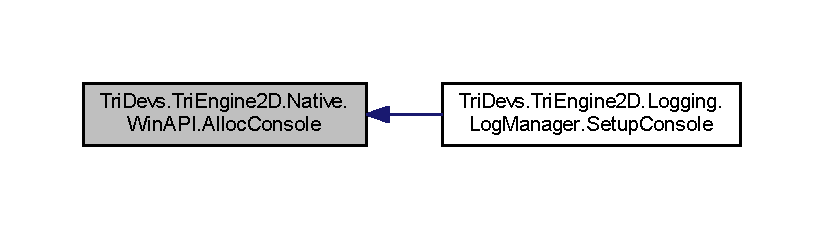
\includegraphics[width=350pt]{class_tri_devs_1_1_tri_engine2_d_1_1_native_1_1_win_a_p_i_a00f0889a729e989fbefd8267a20a1c06_icgraph}
\end{center}
\end{figure}


\hypertarget{class_tri_devs_1_1_tri_engine2_d_1_1_native_1_1_win_a_p_i_a14d148cdaa742fd0d25fd962f6c1f8c4}{\index{Tri\-Devs\-::\-Tri\-Engine2\-D\-::\-Native\-::\-Win\-A\-P\-I@{Tri\-Devs\-::\-Tri\-Engine2\-D\-::\-Native\-::\-Win\-A\-P\-I}!Free\-Console@{Free\-Console}}
\index{Free\-Console@{Free\-Console}!TriDevs::TriEngine2D::Native::WinAPI@{Tri\-Devs\-::\-Tri\-Engine2\-D\-::\-Native\-::\-Win\-A\-P\-I}}
\subsubsection[{Free\-Console}]{\setlength{\rightskip}{0pt plus 5cm}static int Tri\-Devs.\-Tri\-Engine2\-D.\-Native.\-Win\-A\-P\-I.\-Free\-Console (
\begin{DoxyParamCaption}
{}
\end{DoxyParamCaption}
)}}\label{class_tri_devs_1_1_tri_engine2_d_1_1_native_1_1_win_a_p_i_a14d148cdaa742fd0d25fd962f6c1f8c4}


Detaches the calling process from its console. 

\begin{DoxyReturn}{Returns}
If the function succeeds, the return value is nonzero. If the function fails, the return value is zero. To get extended error information, call Get\-Last\-Error. 
\end{DoxyReturn}


Here is the caller graph for this function\-:\nopagebreak
\begin{figure}[H]
\begin{center}
\leavevmode
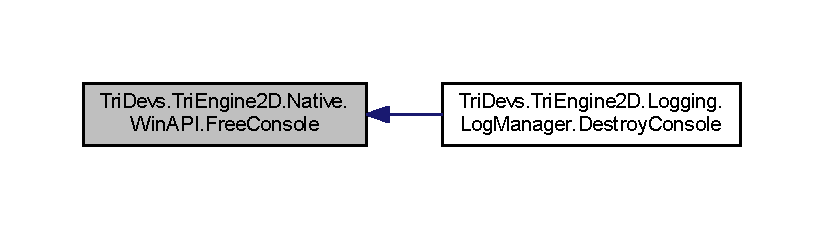
\includegraphics[width=350pt]{class_tri_devs_1_1_tri_engine2_d_1_1_native_1_1_win_a_p_i_a14d148cdaa742fd0d25fd962f6c1f8c4_icgraph}
\end{center}
\end{figure}


\hypertarget{class_tri_devs_1_1_tri_engine2_d_1_1_native_1_1_win_a_p_i_a7617bf77270291625f566cf21294d518}{\index{Tri\-Devs\-::\-Tri\-Engine2\-D\-::\-Native\-::\-Win\-A\-P\-I@{Tri\-Devs\-::\-Tri\-Engine2\-D\-::\-Native\-::\-Win\-A\-P\-I}!Get\-Std\-Handle@{Get\-Std\-Handle}}
\index{Get\-Std\-Handle@{Get\-Std\-Handle}!TriDevs::TriEngine2D::Native::WinAPI@{Tri\-Devs\-::\-Tri\-Engine2\-D\-::\-Native\-::\-Win\-A\-P\-I}}
\subsubsection[{Get\-Std\-Handle}]{\setlength{\rightskip}{0pt plus 5cm}static Int\-Ptr Tri\-Devs.\-Tri\-Engine2\-D.\-Native.\-Win\-A\-P\-I.\-Get\-Std\-Handle (
\begin{DoxyParamCaption}
\item[{int}]{n\-Std\-Handle}
\end{DoxyParamCaption}
)}}\label{class_tri_devs_1_1_tri_engine2_d_1_1_native_1_1_win_a_p_i_a7617bf77270291625f566cf21294d518}


Retrieves a handle to the specified standard device (standard input, standard output, or standard error). 


\begin{DoxyParams}{Parameters}
{\em n\-Std\-Handle} & The standard device.\\
\hline
\end{DoxyParams}
\begin{DoxyReturn}{Returns}
If the function succeeds, the return value is a handle to the specified device, or a redirected handle set by a previous call to Set\-Std\-Handle. The handle has G\-E\-N\-E\-R\-I\-C\-\_\-\-R\-E\-A\-D and G\-E\-N\-E\-R\-I\-C\-\_\-\-W\-R\-I\-T\-E access rights, unless the application has used Set\-Std\-Handle to set a standard handle with lesser access. If the function fails, the return value is I\-N\-V\-A\-L\-I\-D\-\_\-\-H\-A\-N\-D\-L\-E\-\_\-\-V\-A\-L\-U\-E. To get extended error information, call Get\-Last\-Error. If an application does not have associated standard handles, such as a service running on an interactive desktop, and has not redirected them, the return value is N\-U\-L\-L. 
\end{DoxyReturn}


Here is the caller graph for this function\-:\nopagebreak
\begin{figure}[H]
\begin{center}
\leavevmode
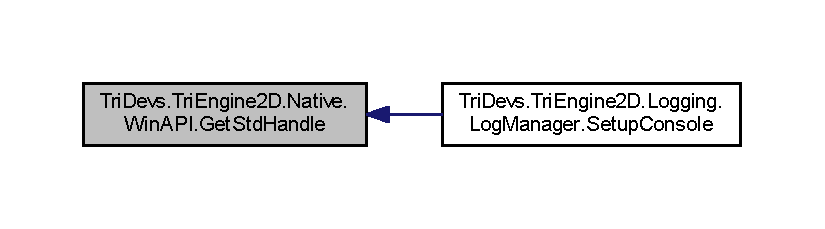
\includegraphics[width=350pt]{class_tri_devs_1_1_tri_engine2_d_1_1_native_1_1_win_a_p_i_a7617bf77270291625f566cf21294d518_icgraph}
\end{center}
\end{figure}




\subsection{Member Data Documentation}
\hypertarget{class_tri_devs_1_1_tri_engine2_d_1_1_native_1_1_win_a_p_i_a83ef0d2539e95cc640d8e1f1216beec5}{\index{Tri\-Devs\-::\-Tri\-Engine2\-D\-::\-Native\-::\-Win\-A\-P\-I@{Tri\-Devs\-::\-Tri\-Engine2\-D\-::\-Native\-::\-Win\-A\-P\-I}!C\-O\-D\-E\-\_\-\-P\-A\-G\-E@{C\-O\-D\-E\-\_\-\-P\-A\-G\-E}}
\index{C\-O\-D\-E\-\_\-\-P\-A\-G\-E@{C\-O\-D\-E\-\_\-\-P\-A\-G\-E}!TriDevs::TriEngine2D::Native::WinAPI@{Tri\-Devs\-::\-Tri\-Engine2\-D\-::\-Native\-::\-Win\-A\-P\-I}}
\subsubsection[{C\-O\-D\-E\-\_\-\-P\-A\-G\-E}]{\setlength{\rightskip}{0pt plus 5cm}const int Tri\-Devs.\-Tri\-Engine2\-D.\-Native.\-Win\-A\-P\-I.\-C\-O\-D\-E\-\_\-\-P\-A\-G\-E = 437}}\label{class_tri_devs_1_1_tri_engine2_d_1_1_native_1_1_win_a_p_i_a83ef0d2539e95cc640d8e1f1216beec5}


The code page to use for the console. 

\hypertarget{class_tri_devs_1_1_tri_engine2_d_1_1_native_1_1_win_a_p_i_a19ebb40d1edf46781ea0fdf4a9c94e8b}{\index{Tri\-Devs\-::\-Tri\-Engine2\-D\-::\-Native\-::\-Win\-A\-P\-I@{Tri\-Devs\-::\-Tri\-Engine2\-D\-::\-Native\-::\-Win\-A\-P\-I}!S\-T\-D\-\_\-\-O\-U\-T\-P\-U\-T\-\_\-\-H\-A\-N\-D\-L\-E@{S\-T\-D\-\_\-\-O\-U\-T\-P\-U\-T\-\_\-\-H\-A\-N\-D\-L\-E}}
\index{S\-T\-D\-\_\-\-O\-U\-T\-P\-U\-T\-\_\-\-H\-A\-N\-D\-L\-E@{S\-T\-D\-\_\-\-O\-U\-T\-P\-U\-T\-\_\-\-H\-A\-N\-D\-L\-E}!TriDevs::TriEngine2D::Native::WinAPI@{Tri\-Devs\-::\-Tri\-Engine2\-D\-::\-Native\-::\-Win\-A\-P\-I}}
\subsubsection[{S\-T\-D\-\_\-\-O\-U\-T\-P\-U\-T\-\_\-\-H\-A\-N\-D\-L\-E}]{\setlength{\rightskip}{0pt plus 5cm}const int Tri\-Devs.\-Tri\-Engine2\-D.\-Native.\-Win\-A\-P\-I.\-S\-T\-D\-\_\-\-O\-U\-T\-P\-U\-T\-\_\-\-H\-A\-N\-D\-L\-E = -\/11}}\label{class_tri_devs_1_1_tri_engine2_d_1_1_native_1_1_win_a_p_i_a19ebb40d1edf46781ea0fdf4a9c94e8b}


The standard output device. Initially, this is the active console screen buffer, C\-O\-N\-O\-U\-T\$. 



The documentation for this class was generated from the following file\-:\begin{DoxyCompactItemize}
\item 
Tri\-Devs.\-Tri\-Engine2\-D/\-Native/\hyperlink{_win_a_p_i_8cs}{Win\-A\-P\-I.\-cs}\end{DoxyCompactItemize}

\chapter{File Documentation}
\hypertarget{_r_e_a_d_m_e_8md}{\section{R\-E\-A\-D\-M\-E.\-md File Reference}
\label{_r_e_a_d_m_e_8md}\index{R\-E\-A\-D\-M\-E.\-md@{R\-E\-A\-D\-M\-E.\-md}}
}

\hypertarget{_enumeration_extensions_8cs}{\section{Tri\-Devs.\-Tri\-Engine2\-D/\-Extensions/\-Enumeration\-Extensions.cs File Reference}
\label{_enumeration_extensions_8cs}\index{Tri\-Devs.\-Tri\-Engine2\-D/\-Extensions/\-Enumeration\-Extensions.\-cs@{Tri\-Devs.\-Tri\-Engine2\-D/\-Extensions/\-Enumeration\-Extensions.\-cs}}
}
\subsection*{Classes}
\begin{DoxyCompactItemize}
\item 
class \hyperlink{class_tri_devs_1_1_tri_engine2_d_1_1_extensions_1_1_enumeration_extensions}{Tri\-Devs.\-Tri\-Engine2\-D.\-Extensions.\-Enumeration\-Extensions}
\begin{DoxyCompactList}\small\item\em \hyperlink{namespace_tri_devs_1_1_tri_engine2_d_1_1_extensions}{Extensions} for System.\-Enum. \end{DoxyCompactList}\end{DoxyCompactItemize}
\subsection*{Namespaces}
\begin{DoxyCompactItemize}
\item 
package \hyperlink{namespace_tri_devs_1_1_tri_engine2_d_1_1_extensions}{Tri\-Devs.\-Tri\-Engine2\-D.\-Extensions}
\end{DoxyCompactItemize}

\hypertarget{_string_extensions_8cs}{\section{Tri\-Devs.\-Tri\-Engine2\-D/\-Extensions/\-String\-Extensions.cs File Reference}
\label{_string_extensions_8cs}\index{Tri\-Devs.\-Tri\-Engine2\-D/\-Extensions/\-String\-Extensions.\-cs@{Tri\-Devs.\-Tri\-Engine2\-D/\-Extensions/\-String\-Extensions.\-cs}}
}
\subsection*{Classes}
\begin{DoxyCompactItemize}
\item 
class \hyperlink{class_tri_devs_1_1_tri_engine2_d_1_1_extensions_1_1_string_extensions}{Tri\-Devs.\-Tri\-Engine2\-D.\-Extensions.\-String\-Extensions}
\begin{DoxyCompactList}\small\item\em \hyperlink{namespace_tri_devs_1_1_tri_engine2_d_1_1_extensions}{Extensions} for System.\-String \end{DoxyCompactList}\end{DoxyCompactItemize}
\subsection*{Namespaces}
\begin{DoxyCompactItemize}
\item 
package \hyperlink{namespace_tri_devs_1_1_tri_engine2_d_1_1_extensions}{Tri\-Devs.\-Tri\-Engine2\-D.\-Extensions}
\end{DoxyCompactItemize}

\hypertarget{_i_o_8cs}{\section{Tri\-Devs.\-Tri\-Engine/\-Helpers/\-I\-O.cs File Reference}
\label{_i_o_8cs}\index{Tri\-Devs.\-Tri\-Engine/\-Helpers/\-I\-O.\-cs@{Tri\-Devs.\-Tri\-Engine/\-Helpers/\-I\-O.\-cs}}
}
\subsection*{Classes}
\begin{DoxyCompactItemize}
\item 
class \hyperlink{class_tri_devs_1_1_tri_engine_1_1_helpers_1_1_i_o}{Tri\-Devs.\-Tri\-Engine.\-Helpers.\-I\-O}
\begin{DoxyCompactList}\small\item\em Provides various helper functions for doing \hyperlink{class_tri_devs_1_1_tri_engine_1_1_helpers_1_1_i_o}{I\-O} operations. \end{DoxyCompactList}\end{DoxyCompactItemize}
\subsection*{Namespaces}
\begin{DoxyCompactItemize}
\item 
package \hyperlink{namespace_tri_devs_1_1_tri_engine_1_1_helpers}{Tri\-Devs.\-Tri\-Engine.\-Helpers}
\end{DoxyCompactItemize}

\hypertarget{_threading_8cs}{\section{Tri\-Devs.\-Tri\-Engine/\-Helpers/\-Threading.cs File Reference}
\label{_threading_8cs}\index{Tri\-Devs.\-Tri\-Engine/\-Helpers/\-Threading.\-cs@{Tri\-Devs.\-Tri\-Engine/\-Helpers/\-Threading.\-cs}}
}
\subsection*{Classes}
\begin{DoxyCompactItemize}
\item 
class \hyperlink{class_tri_devs_1_1_tri_engine_1_1_helpers_1_1_threading}{Tri\-Devs.\-Tri\-Engine.\-Helpers.\-Threading}
\begin{DoxyCompactList}\small\item\em Provides various helper functions for doing threading operations. \end{DoxyCompactList}\end{DoxyCompactItemize}
\subsection*{Namespaces}
\begin{DoxyCompactItemize}
\item 
package \hyperlink{namespace_tri_devs_1_1_tri_engine_1_1_helpers}{Tri\-Devs.\-Tri\-Engine.\-Helpers}
\end{DoxyCompactItemize}

\hypertarget{_i_input_manager_8cs}{\section{Tri\-Devs.\-Tri\-Engine2\-D/\-Input/\-I\-Input\-Manager.cs File Reference}
\label{_i_input_manager_8cs}\index{Tri\-Devs.\-Tri\-Engine2\-D/\-Input/\-I\-Input\-Manager.\-cs@{Tri\-Devs.\-Tri\-Engine2\-D/\-Input/\-I\-Input\-Manager.\-cs}}
}
\subsection*{Classes}
\begin{DoxyCompactItemize}
\item 
interface \hyperlink{interface_tri_devs_1_1_tri_engine2_d_1_1_input_1_1_i_input_manager}{Tri\-Devs.\-Tri\-Engine2\-D.\-Input.\-I\-Input\-Manager}
\begin{DoxyCompactList}\small\item\em Provides various methods to query input devices like the keyboard. \end{DoxyCompactList}\end{DoxyCompactItemize}
\subsection*{Namespaces}
\begin{DoxyCompactItemize}
\item 
package \hyperlink{namespace_tri_devs_1_1_tri_engine2_d_1_1_input}{Tri\-Devs.\-Tri\-Engine2\-D.\-Input}
\end{DoxyCompactItemize}

\hypertarget{_input_manager_8cs}{\section{Tri\-Devs.\-Tri\-Engine2\-D/\-Input/\-Input\-Manager.cs File Reference}
\label{_input_manager_8cs}\index{Tri\-Devs.\-Tri\-Engine2\-D/\-Input/\-Input\-Manager.\-cs@{Tri\-Devs.\-Tri\-Engine2\-D/\-Input/\-Input\-Manager.\-cs}}
}
\subsection*{Classes}
\begin{DoxyCompactItemize}
\item 
class \hyperlink{class_tri_devs_1_1_tri_engine2_d_1_1_input_1_1_input_manager}{Tri\-Devs.\-Tri\-Engine2\-D.\-Input.\-Input\-Manager}
\begin{DoxyCompactList}\small\item\em \hyperlink{namespace_tri_devs_1_1_tri_engine2_d_1_1_input}{Input} manager interfacing with input methods provided by a Game\-Window. \end{DoxyCompactList}\end{DoxyCompactItemize}
\subsection*{Namespaces}
\begin{DoxyCompactItemize}
\item 
package \hyperlink{namespace_tri_devs_1_1_tri_engine2_d_1_1_input}{Tri\-Devs.\-Tri\-Engine2\-D.\-Input}
\end{DoxyCompactItemize}

\hypertarget{_null_input_manager_8cs}{\section{Tri\-Devs.\-Tri\-Engine/\-Input/\-Null\-Input\-Manager.cs File Reference}
\label{_null_input_manager_8cs}\index{Tri\-Devs.\-Tri\-Engine/\-Input/\-Null\-Input\-Manager.\-cs@{Tri\-Devs.\-Tri\-Engine/\-Input/\-Null\-Input\-Manager.\-cs}}
}
\subsection*{Classes}
\begin{DoxyCompactItemize}
\item 
class \hyperlink{class_tri_devs_1_1_tri_engine_1_1_input_1_1_null_input_manager}{Tri\-Devs.\-Tri\-Engine.\-Input.\-Null\-Input\-Manager}
\begin{DoxyCompactList}\small\item\em Used as a fallback \hyperlink{class_tri_devs_1_1_tri_engine_1_1_input_1_1_input_manager}{Input\-Manager} object when the service locator fails to find one. \end{DoxyCompactList}\end{DoxyCompactItemize}
\subsection*{Namespaces}
\begin{DoxyCompactItemize}
\item 
package \hyperlink{namespace_tri_devs_1_1_tri_engine_1_1_input}{Tri\-Devs.\-Tri\-Engine.\-Input}
\end{DoxyCompactItemize}

\hypertarget{_log_manager_8cs}{\section{Tri\-Devs.\-Tri\-Engine2\-D/\-Logging/\-Log\-Manager.cs File Reference}
\label{_log_manager_8cs}\index{Tri\-Devs.\-Tri\-Engine2\-D/\-Logging/\-Log\-Manager.\-cs@{Tri\-Devs.\-Tri\-Engine2\-D/\-Logging/\-Log\-Manager.\-cs}}
}
\subsection*{Classes}
\begin{DoxyCompactItemize}
\item 
class \hyperlink{class_tri_devs_1_1_tri_engine2_d_1_1_logging_1_1_log_manager}{Tri\-Devs.\-Tri\-Engine2\-D.\-Logging.\-Log\-Manager}
\begin{DoxyCompactList}\small\item\em Class to manage logging. I\-Log interfaces should be obtained from this class' methods, as opposed to calling default log4net methods. \end{DoxyCompactList}\end{DoxyCompactItemize}
\subsection*{Namespaces}
\begin{DoxyCompactItemize}
\item 
package \hyperlink{namespace_tri_devs_1_1_tri_engine2_d_1_1_logging}{Tri\-Devs.\-Tri\-Engine2\-D.\-Logging}
\end{DoxyCompactItemize}

\hypertarget{_helpers_8cs}{\section{Tri\-Devs.\-Tri\-Engine/\-Native/\-Helpers.cs File Reference}
\label{_helpers_8cs}\index{Tri\-Devs.\-Tri\-Engine/\-Native/\-Helpers.\-cs@{Tri\-Devs.\-Tri\-Engine/\-Native/\-Helpers.\-cs}}
}
\subsection*{Classes}
\begin{DoxyCompactItemize}
\item 
class \hyperlink{class_tri_devs_1_1_tri_engine_1_1_native_1_1_helpers}{Tri\-Devs.\-Tri\-Engine.\-Native.\-Helpers}
\begin{DoxyCompactList}\small\item\em Helper class with various methods to help native coding and debugging. \end{DoxyCompactList}\end{DoxyCompactItemize}
\subsection*{Namespaces}
\begin{DoxyCompactItemize}
\item 
package \hyperlink{namespace_tri_devs_1_1_tri_engine_1_1_native}{Tri\-Devs.\-Tri\-Engine.\-Native}
\end{DoxyCompactItemize}

\hypertarget{_win_a_p_i_8cs}{\section{Tri\-Devs.\-Tri\-Engine2\-D/\-Native/\-Win\-A\-P\-I.cs File Reference}
\label{_win_a_p_i_8cs}\index{Tri\-Devs.\-Tri\-Engine2\-D/\-Native/\-Win\-A\-P\-I.\-cs@{Tri\-Devs.\-Tri\-Engine2\-D/\-Native/\-Win\-A\-P\-I.\-cs}}
}
\subsection*{Classes}
\begin{DoxyCompactItemize}
\item 
class \hyperlink{class_tri_devs_1_1_tri_engine2_d_1_1_native_1_1_win_a_p_i}{Tri\-Devs.\-Tri\-Engine2\-D.\-Native.\-Win\-A\-P\-I}
\begin{DoxyCompactList}\small\item\em Holds various \hyperlink{class_tri_devs_1_1_tri_engine2_d_1_1_native_1_1_win_a_p_i}{Win\-A\-P\-I} stuff. \end{DoxyCompactList}\end{DoxyCompactItemize}
\subsection*{Namespaces}
\begin{DoxyCompactItemize}
\item 
package \hyperlink{namespace_tri_devs_1_1_tri_engine2_d_1_1_native}{Tri\-Devs.\-Tri\-Engine2\-D.\-Native}
\end{DoxyCompactItemize}

\hypertarget{_point_8cs}{\section{Tri\-Devs.\-Tri\-Engine/\-Point.cs File Reference}
\label{_point_8cs}\index{Tri\-Devs.\-Tri\-Engine/\-Point.\-cs@{Tri\-Devs.\-Tri\-Engine/\-Point.\-cs}}
}
\subsection*{Classes}
\begin{DoxyCompactItemize}
\item 
struct \hyperlink{struct_tri_devs_1_1_tri_engine_1_1_point_3_01_t_01_4}{Tri\-Devs.\-Tri\-Engine.\-Point$<$ T $>$}
\begin{DoxyCompactList}\small\item\em A struct representing an X/\-Y coordinate. \end{DoxyCompactList}\end{DoxyCompactItemize}
\subsection*{Namespaces}
\begin{DoxyCompactItemize}
\item 
package \hyperlink{namespace_tri_devs_1_1_tri_engine}{Tri\-Devs.\-Tri\-Engine}
\end{DoxyCompactItemize}

\hypertarget{_assembly_info_8cs}{\section{Tri\-Devs.\-Tri\-Engine/\-Properties/\-Assembly\-Info.cs File Reference}
\label{_assembly_info_8cs}\index{Tri\-Devs.\-Tri\-Engine/\-Properties/\-Assembly\-Info.\-cs@{Tri\-Devs.\-Tri\-Engine/\-Properties/\-Assembly\-Info.\-cs}}
}

\hypertarget{_serializer_8cs}{\section{Tri\-Devs.\-Tri\-Engine2\-D/\-Serializing/\-Serializer.cs File Reference}
\label{_serializer_8cs}\index{Tri\-Devs.\-Tri\-Engine2\-D/\-Serializing/\-Serializer.\-cs@{Tri\-Devs.\-Tri\-Engine2\-D/\-Serializing/\-Serializer.\-cs}}
}
\subsection*{Classes}
\begin{DoxyCompactItemize}
\item 
class \hyperlink{class_tri_devs_1_1_tri_engine2_d_1_1_serializing_1_1_serializer}{Tri\-Devs.\-Tri\-Engine2\-D.\-Serializing.\-Serializer}
\begin{DoxyCompactList}\small\item\em Provides serialization methods. \end{DoxyCompactList}\end{DoxyCompactItemize}
\subsection*{Namespaces}
\begin{DoxyCompactItemize}
\item 
package \hyperlink{namespace_tri_devs_1_1_tri_engine2_d_1_1_serializing}{Tri\-Devs.\-Tri\-Engine2\-D.\-Serializing}
\end{DoxyCompactItemize}

\hypertarget{_services_8cs}{\section{Tri\-Devs.\-Tri\-Engine/\-Services.cs File Reference}
\label{_services_8cs}\index{Tri\-Devs.\-Tri\-Engine/\-Services.\-cs@{Tri\-Devs.\-Tri\-Engine/\-Services.\-cs}}
}
\subsection*{Classes}
\begin{DoxyCompactItemize}
\item 
class \hyperlink{class_tri_devs_1_1_tri_engine_1_1_services}{Tri\-Devs.\-Tri\-Engine.\-Services}
\begin{DoxyCompactList}\small\item\em Provides different game-\/related service interfaces. \end{DoxyCompactList}\end{DoxyCompactItemize}
\subsection*{Namespaces}
\begin{DoxyCompactItemize}
\item 
package \hyperlink{namespace_tri_devs_1_1_tri_engine}{Tri\-Devs.\-Tri\-Engine}
\end{DoxyCompactItemize}

\hypertarget{_version_8cs}{\section{Tri\-Devs.\-Tri\-Engine/\-Version.cs File Reference}
\label{_version_8cs}\index{Tri\-Devs.\-Tri\-Engine/\-Version.\-cs@{Tri\-Devs.\-Tri\-Engine/\-Version.\-cs}}
}
\subsection*{Classes}
\begin{DoxyCompactItemize}
\item 
class \hyperlink{class_tri_devs_1_1_tri_engine_1_1_version}{Tri\-Devs.\-Tri\-Engine.\-Version}
\begin{DoxyCompactList}\small\item\em \hyperlink{class_tri_devs_1_1_tri_engine_1_1_version}{Version} class specifiying the version of this project. \end{DoxyCompactList}\end{DoxyCompactItemize}
\subsection*{Namespaces}
\begin{DoxyCompactItemize}
\item 
package \hyperlink{namespace_tri_devs_1_1_tri_engine}{Tri\-Devs.\-Tri\-Engine}
\end{DoxyCompactItemize}

\addcontentsline{toc}{part}{Index}
\printindex
\end{document}
